\chapter{Kiến thức toán học nền tảng}

\ % Lùi đầu dòng

Chương này bao gồm các kiến thức toán học cần thiết để xây dựng lí thuyết của môn vật lí (hoặc ít nhất để đọc tài liệu này), giả sử rằng bạn đọc đã có một chút kiến thức đại số và hình học trung học phổ thông từ ghế nhà trường. Một điều cần lưu ý là chương này sẽ bao hàm những phần không nằm trong chương trình trung học phổ thông và có thể cả chương trình đại học. Mặc dù rằng là tác giả đã bao hàm rất nhiều toán trong chương, nhưng tác giả không có ý định viết để thay thế toàn bộ giáo trình toán. Các cuốn giải tích, đại số tuyến tính, hình học phẳng, hình học không gian, xác suất, và các cuốn giáo trình toán khác đều có vị trí đứng của chúng. Điều mà tác giả mong muốn tài liệu này có được chính là sự tổng hợp của kiến thức toán sao cho phù hợp với các ngành vật lí và sự bù đắp cho những lỗ hổng mà tác giả còn thấy ở tài liệu toán hiện hành ở Việt Nam. Kể như, trong tài liệu này, khi nhắc về hàm số, không có phần về đơn ánh hay toàn ánh. Những khái niệm này là vô cùng quan trọng nếu tập trung chứng minh chặt chẽ các tính chất liên quan đến hàm số, nhưng không phục vụ nhiều trong ứng dụng thực tiễn. Thay vào đó, tài liệu được đưa thêm những dạng bài tập, như các dạng bài liên quan đến hàm số rời rạc được cho dưới dạng bảng, mà bạn đọc ít khả năng nhìn thấy ở trong những tài liệu khác. Không phải dạng bài tập mới là để bạn đọc trở nên hứng thú hơn, bởi dĩ tác giả khi soạn đáp án còn thấy chán, mà điều quan trọng là tìm ra nguyên nhân từ cái chán đó, và tìm cách chấm dứt triệt để cái chán bằng việc kết nối các bài toán lại với nhau, và rút ra một quy luật tổng quát giữa chúng. Suy cho cùng, sau khi bạn đọc làm nhiều bài tập, tác giả kì vọng, hơn cả việc bạn đọc tính toán nhanh và thành thạo (đương nhiên điều này cũng rất tốt), chính là việc hiểu rõ bản chất của các mảng lí thuyết và từ đó ứng dụng vào các trường hợp khác nhau.

Thông thường, các tài liệu vật lí sẽ lược qua hay tối giản phần toán, với ba ngầm định. Thứ nhất, sẽ có tài liệu toán ứng dụng đi kèm với tài liệu vật lí. Thứ hai, vật lí không dùng nhiều đến lí thuyết toán chuyên sâu hay chứng minh chặt chẽ. Và thứ ba, vật lí không nên dùng đến các tính toán phức tạp mà nên tập trung nhiều vào phần thông hiểu lí thuyết và ứng dụng đời sống. Tuy nhiên, tác giả lại không định hướng tài liệu đi theo những quan điểm này. Các mô hình vật lí đều có toán học phụ trợ đằng sau và chứng minh toán học mới là thứ xây dựng mô hình để dự đoán tương lai. Lấy ví dụ, thuyết tương đối rộng của Anh-xtanh\footnote{Albert Einstein (1879 - 1955)}. Đây là thuyết có thể nói được kiểm chứng thực nghiệm nhiều lần nhất trong vật lí, và giống rất nhiều công trình vật lí hiện đại khác, được xây dựng từ bút, giấy, và nhiều công cụ toán và một chút góc nhìn sáng tạo của vật lí. Quay trở về hiện tại, theo tác giả, nếu như nhà vật lí hay kĩ sư mà không làm được toán cao cấp, thì có lẽ họ nên chuyển nghề. Cho nên, trong tài liệu này, tác giả không chỉ đưa nhiều toán, mà còn đưa ra toán theo con đường khác với con đường thông thường. Các lí thuyết bình thường được đặt ở cùng chỗ thì sẽ tách nhau ra, không phải là cố tình phức tạp hóa, mà là để thể hiện tính mạch lạc của toán, nhấn mạnh rằng toán có thể tư duy được chứ không chỉ là thuộc lòng một cách \dblquote{tôn giáo hóa}. Tác giả vẫn đưa một số lí thuyết dựa trên ngôn ngữ đời thường, nhưng nếu có thể, tác giả sẽ đưa định nghĩa hay chứng minh theo toán học thuần túy, dựa trên những lí thuyết đã có trước đó.

Có thể những kiến thức này đã cũ và bạn đọc chỉ muốn làm nóng lại kiến thức ở những phần cần thiết, thì bạn đọc có thể bỏ qua một vài phần của chương này. Nhưng nếu bạn đọc thấy những kiến thức này còn mới, còn nhiều lỗ hổng, thì bạn đọc nên đọc kĩ lưỡng. Hi vọng từ lí thuyết và bài tập, bạn đọc có thể hiểu được góc nhìn của tác giả về toán, và tự xây dựng cho mình một ma trận kiến thức riêng để phục vụ sau này.

% \section{Đồ thị}

\subsection{Trục số một chiều}

\ % Lùi đầu dòng

Đồ thị là cầu nối đầu tiên giữa đại số và hình học mà chắc là bạn đọc đã được học. Thông thường, nhắc đến đồ thị, chúng thường được dùng để biểu thị mặt phẳng hai chiều hoặc không gian ba chiều. Nhưng, đồ thị cơ bản nhất chỉ có một chiều, hay tên gọi khác là \emph{trục số}. 

\def \pointSize {1.5pt}

\begin{wrapfigure}{r}{0.4\textwidth}
   \centering
   \begin{tikzpicture}
      \draw[->] (-3,0) -- (2,0) node[right] {Trục số};
      \filldraw (0, 0) circle (\pointSize) node[below] {$O(0)$};
      \filldraw (1.5, 0) circle (\pointSize) node[below] {$P(x_P)$};
      \filldraw (-1.5, 0) circle (\pointSize) node[below] {$P_-(-x_P)$};
   \end{tikzpicture}
   \caption{Trục số một chiều}
   \label{fig:do_thi:truc_so:truc_so_mot_chieu}
\end{wrapfigure}

Đặt một điểm trên trục làm gốc tọa độ $0$, từ đó chúng ta có thể biểu diễn mọi số thực trên trục số này. Nói một cách không chính thống, với một số $x_P$ dương bất kì, đánh dấu cách $O$ một đoạn bằng $x_P$ đơn vị độ dài theo hướng trục, chúng ta có điểm $P$ biểu diễn $x_P$. Viết tắt cách biểu diễn, được $P(x_P)$. Ngược lại, nếu chúng ta muốn đánh dấu số $x_{P_-}=-x_P$ mang giá trị âm, chúng ta dịch ngược lại chiều trục như trên hình \ref{fig:do_thi:truc_so:truc_so_mot_chieu}.

\begin{wrapfigure}{r}{0.4\textwidth}
   \centering
   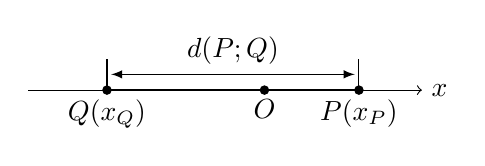
\begin{tikzpicture}
      \draw[->] (-3,0) -- (2,0) node[right] {$x$};
      \filldraw (0, 0) circle (\pointSize) node[below] {$O$};
      \pgfmathsetmacro{\xP}{1.2}
      \pgfmathsetmacro{\xQ}{-2}
      \pgfmathsetmacro{\h}{0.4}
      \filldraw (\xP, 0) circle (\pointSize) node[below] {$P(x_P)$};
      \filldraw (\xQ, 0) circle (\pointSize) node[below] {$Q(x_Q)$};
      \draw[thick] (\xQ,0) -- (\xP,0);
      \node[above] at ({(\xP+\xQ)/2}, {\h/2}) {$d(P;Q)$};
      \draw (\xP,0) -- (\xP,\h);
      \draw (\xQ,0) -- (\xQ,\h);
      \draw[<->, >=latex, shorten >=\pointSize, shorten <=\pointSize] (\xP,{\h/2}) -- (\xQ,{\h/2});
   \end{tikzpicture}
   \caption{Khoảng cách trên trục số}
   \label{fig:do_thi:truc_so:khoang_cach_truc_so}
\end{wrapfigure}

Khi có nhiều điểm ở trên đồ thị, chúng ta sẽ mong muốn tính những thông số liên quan tới những điểm đó. Do kiến thức toán hiện tại đang bị giới hạn, chúng ta sẽ chỉ tập trung vào một đặc điểm nhất định, \emph{khoảng cách}. Trên một trục số như hình \ref{fig:do_thi:truc_so:khoang_cach_truc_so}, cho hai điểm $P(x_P)$ và $Q(x_Q)$, khoảng cách giữa chúng là $$d(P;Q)=\sqrt{(x_P-x_Q)^2}=|x_P-x_Q|.$$

\exercise[ex:0.1] Biểu diễn nhóm các điểm sau trên trục số. Tính khoảng cách giữa hai điểm phân biệt bất kì trong nhóm đó.
\begin{enumerate}
   \item $A(2)$, $B(-3)$, và $C(4)$;
   \item $D(\pi)$, $E(-\pi)$, $F(0)$, và $G\left(\frac{\pi}{2}\right)$;
   \item $H(0{,}\overline{3})$ và $I(\sqrt{2})$;
   \item $J\left(\frac{355}{113}\right)$, $K\left(\frac{9801}{2206\sqrt{2}}\right)$ và $L\left(\sqrt[4]{\frac{2143}{22}}\right)$;
   \item $M(x)$ và $N(2x)$ với $x\in\mathbb{R}$.
\end{enumerate}

\solution[ex:0.1] 
\begin{figure}[h]
   \centering
   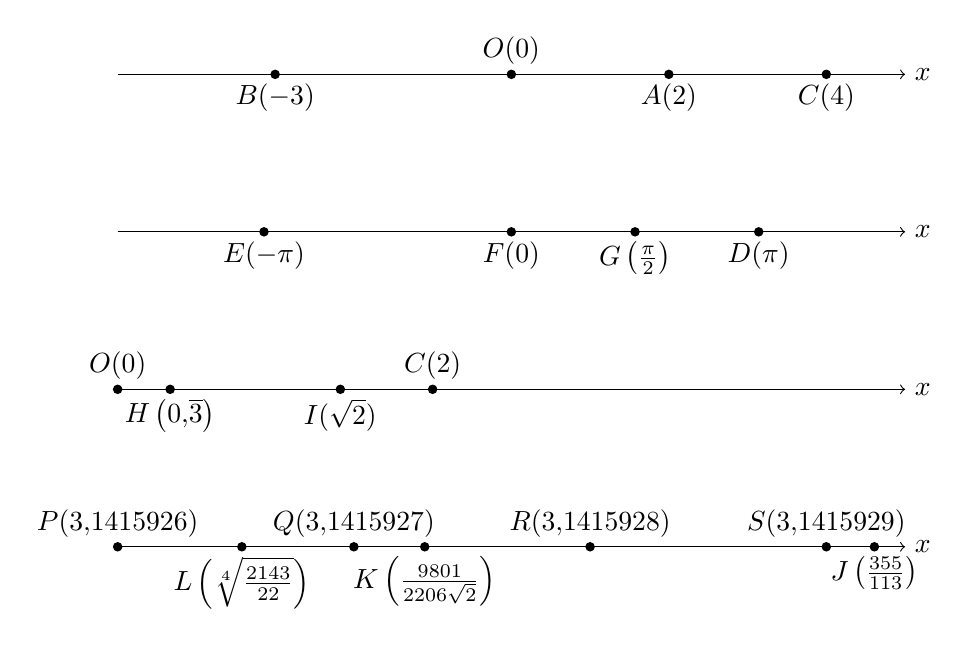
\begin{tikzpicture}[scale=1]

      \begin{scope}[yshift=2cm]
         \draw[->] (-5,0) -- (5,0) node[right] {$x$};
         \filldraw (0, 0) circle (\pointSize) node[above] {$O(0)$};
         \filldraw (2, 0) circle (\pointSize) node[below] {$A(2)$};
         \filldraw (-3, 0) circle (\pointSize) node[below] {$B(-3)$};
         \filldraw (4, 0) circle (\pointSize) node[below] {$C(4)$};
      \end{scope}

      \begin{scope}[yshift=0cm]
         \draw[->] (-5,0) -- (5,0) node[right] {$x$};
         \filldraw ({pi}, 0) circle (\pointSize) node[below] {$D(\pi)$};
         \filldraw ({-pi}, 0) circle (\pointSize) node[below] {$E(-\pi)$};
         \filldraw (0, 0) circle (\pointSize) node[below] {$F(0)$};
         \filldraw ({pi/2}, 0) circle (\pointSize) node[below] {$G\left(\frac{\pi}{2}\right)$};
      \end{scope}

      \begin{scope}[yshift=-2cm, xshift=-5cm]
         \draw[->] (0,0) -- (10,0) node[right] {$x$};
         \filldraw (0, 0) circle (\pointSize) node[above] {$O(0)$};
         \filldraw ({2/3}, 0) circle (\pointSize) node[below] {$H\left(0{,}\overline{3}\right)$};
         \filldraw ({2*sqrt(2)}, 0) circle (\pointSize) node[below] {$I(\sqrt{2})$};
         \filldraw (4, 0) circle (\pointSize) node[above] {$C(2)$};
      \end{scope}

      \begin{scope}[yshift=-4cm, xshift=-5cm]

         \draw[->] (0,0) -- (10,0) node[right] {$x$};
         \filldraw (0,0) circle (\pointSize) node[above] {$P(3{,}1415926)$};
         \filldraw (3,0) circle (\pointSize) node[above] {$Q(3{,}1415927)$};
         \filldraw (6,0) circle (\pointSize) node[above] {$R(3{,}1415928)$};
         \filldraw (9,0) circle (\pointSize) node[above] {$S(3{,}1415929)$};
         \filldraw (9.61062, 0) circle (\pointSize) node[below] {$J\left(\frac{355}{113}\right)$};
         \filldraw (3.9, 0) circle (\pointSize) node[below] {$K\left(\frac{9801}{2206\sqrt{2}}\right)$};
         \filldraw (1.577475, 0) circle (\pointSize) node[below] {$L\left(\sqrt[4]{\frac{2143}{22}}\right)$};
      \end{scope}

   \end{tikzpicture}
   \caption{Bốn trục số cho các phần từ $1$ đến $4$ của bài \ref{ex:0.1}}
   \label{fig:do_thi:truc_so:bon_truc}
\end{figure}

Ta có đồ thị cho các phần từ $1$ đến $4$ như hình \ref{fig:do_thi:truc_so:bon_truc}.

Cần lưu ý rằng, để biểu diễn thuận lợi nhất, các trục số khi biểu diễn số cần được chọn những tỉ lệ khác nhau và tại những vị trí khác nhau.

Các khoảng cách giữa hai điểm phân biệt đôi một là
\begin{enumerate}
   \item \begin{alignat*}{2}
      &d(A;B) = d(B;A) = \left|2 - (-3)\right| = 5; \\
      &d(B;C) = d(C;B) = \left|4 - (-3)\right| = 7; \\
      &d(C;A) = d(A;C) = \left|4 - 2\right| = 2.
   \end{alignat*}
   \item \begin{alignat*}{2}
      &d(D;E) = d(E;D) = \left|\pi - (-\pi)\right| = 2\pi; \\
      &d(E;F) = d(F;E) = \left|(-\pi) - 0\right| = \pi; \\
      &d(F;G) = d(G;F) = \left|0 - \frac{\pi}{2}\right| = \frac{\pi}{2}; \\
      &d(G;D) = d(D;G) = \left|\frac{\pi}{2} - \pi\right| = \frac{\pi}{2}; \\
      &d(D;F) = d(F;D) = \left|\pi - 0\right| = \pi;\\
      &d(E;G) = d(G;E) = \left|(-\pi) - \frac{\pi}{2}\right| = \frac{3\pi}{2}.
   \end{alignat*}
   \item \begin{alignat*}{2}
      &d(H;I) = d(I;H) = \left|0{,}\overline{3} - \sqrt{2}\right| = \frac{1-3\sqrt{2}}{3}.
   \end{alignat*}
   \item \begin{alignat*}{2}
      &d(J;K) = d(K;J) = \left|\frac{355}{113} - \frac{9801}{2206\sqrt{2}}\right| = \frac{1566260-1107513\sqrt{2}}{498556} \approx 1{,}9034\times 10^{-7}; \\
      &d(K;L) = d(L;K) = \left|\frac{9801}{2206\sqrt{2}} - \sqrt[4]{\frac{2143}{22}}\right| = \frac{107811\sqrt{2}-2206\sqrt[4]{22818664}}{48532} \approx 7{,}7431\times 10^{-8}; \\
      &d(L;J) = d(J;L) = \left|\sqrt[4]{\frac{2143}{22}} - \frac{355}{113}\right| = \frac{7810-113\sqrt[4]{22818664}}{2486} \approx 2{,}6777\times 10^{-7}.
   \end{alignat*}
\end{enumerate}

\begin{figure}[h]
   \centering
   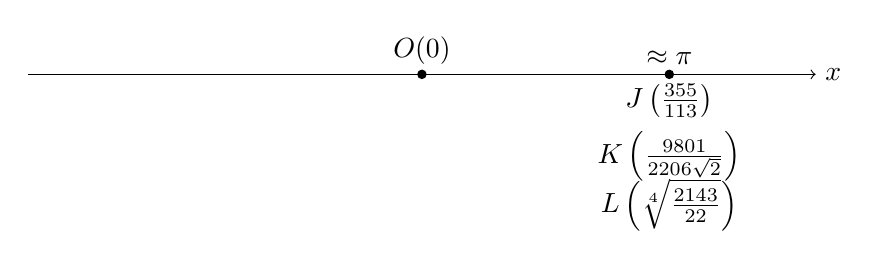
\begin{tikzpicture}[scale=1]
      \draw[->] (-5,0) -- (5,0) node[right] {$x$};
      \filldraw (0, 0) circle (\pointSize) node[above] {$O(0)$};
      \filldraw (pi, 0) circle (\pointSize) node[below] {$J\left(\frac{355}{113}\right)$};
      \node[below] at (pi, -0.6) {$K\left(\frac{9801}{2206\sqrt{2}}\right)$};
      \node[below] at (pi, -1.2) {$L\left(\sqrt[4]{\frac{2143}{22}}\right)$};
      \node[above] at (pi, 0) {$\approx \pi$};
   \end{tikzpicture}
   \caption{Xấp xỉ vị trí điểm trên trục số cho phần $4$ của bài \ref{ex:0.1}}
   \label{fig:truc bon xx}
\end{figure}

Trong vật lí, việc tính toán chính xác đến như ở phần $4$ là không cần thiết và nhiều khi còn không chính xác. Luôn luôn có sai số khi đo đạc, và trong phần lớn trường hợp, khi kết hợp sai số này vào trong tính toán thì các giá trị khoảng cách như trên gần như vô nghĩa. Cho nên, về mặt thực tiễn, chúng ta hoàn toàn có thể thay thế đồ thị của $4$ như hình \ref{fig:truc bon xx} và khi tính khoảng cách, chúng ta có thể tính xấp xỉ là $$d(J,K) = d(K,J) \approx d(K,L) = d(L,K) \approx d(L,J) = d(J,L) \approx 0.$$

\begin{figure}[h]
   \centering
   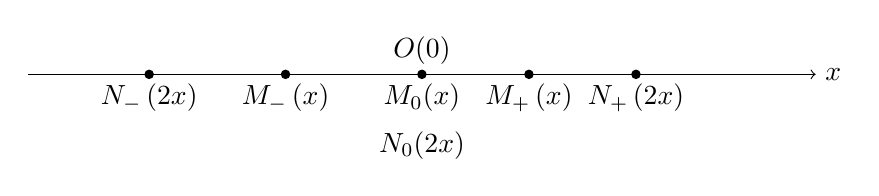
\begin{tikzpicture}[scale=1]
      \draw[->] (-5,0) -- (5,0) node[right] {$x$};
      \filldraw (0, 0) circle (\pointSize) node[above] {$O(0)$} node[below] {$M_0(x)$};
      \node[below] at (0, -0.6) {$N_0(2x)$};
      \filldraw ({e / 2}, 0) circle (\pointSize) node[below] {$M_+\left(x\right)$};
      \filldraw (e, 0) circle (\pointSize) node[below] {$N_+\left(2x\right)$};
      \filldraw ({-sqrt(3)}, 0) circle (\pointSize) node[below] {$M_-\left(x\right)$};
      \filldraw ({-sqrt(3) * 2}, 0) circle (\pointSize) node[below] {$N_-\left(2x\right)$};
   \end{tikzpicture}
   \caption{Ba trường hợp cho vị trí tương đối của $M$, $N$, $O$ cho phần $5$ của bài \ref{ex:0.1}}
   \label{fig:truc phan 5}
\end{figure}

Để vẽ được đồ thị cho phần $5$, chúng ta sẽ xét vị trí tương đối giữa $M$, $N$ kèm theo gốc $O$ để quy chiếu như biểu diễn ở hình \ref{fig:truc phan 5}. Cụ thể, khi $x>0$, điểm $M$ và $N$ được biểu diễn thành hai điểm $M_+$ và $N_+$. Tương tự, khi $x<0$, $M$ và $N$ biểu diễn hai điểm $M_-$ và $N_-$. Một trường hợp đặc biệt là khi $x=0$, $M$ và $N$ đều có tọa độ là $0$, cho nên hai điểm đó và gốc cùng chia sẻ vị trí với nhau.

Khoảng cách giữa hai điểm $M$ và $N$ luôn là $$d(M;N)=d(N;M)=|x-2x|=|x|.$$

\subsection{Mặt phẳng hai chiều và hệ tọa độ vuông góc}

\begin{figure}[h]
   \centering
   \begin{minipage}[b]{0.48\textwidth}
      \centering
      \begin{tikzpicture}
         \draw[->] (-2,0) -- (2,0);
         \draw[->] (0,-2) -- (0,2);
         \node[right] at (2,0) {Trục hoành};
         \node[above] at (0,2) {Trục tung};
         \filldraw (0, 0) circle (1.5pt);
         \node[below left] at (0, 0) {$O(0; 0)$};

         \node at (1,1) {$\boxed{\text{I}}$};
         \node at (-1,1) {$\boxed{\text{II}}$};
         \node at (1,-1) {$\boxed{\text{IV}}$};
         \node at (-1,-1) {$\boxed{\text{III}}$};

         \draw (1,0) -- (1,-0.08) node[below] {$x_P$};
         \draw (0,1.5) -- (-0.08,1.5) node[left] {$y_P$};

         \filldraw (1, 1.5) circle (1.5pt);
         \node[above right] at (1, 1.5) {$P(x_P; y_P)$};

         \draw[dashed] (1, 1.5) -- (1, 0);
         \draw[dashed] (1, 1.5) -- (0, 1.5);
      \end{tikzpicture}
      \caption{Hệ tọa độ vuông góc}
      \label{fig:toa do vuong goc}
   \end{minipage}
   \hfill
   \begin{minipage}[b]{0.48\textwidth}
      \centering
      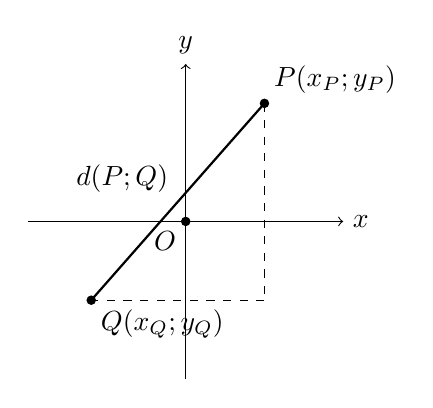
\begin{tikzpicture}
         \draw[->] (-2,0) -- (2,0);
         \draw[->] (0,-2) -- (0,2);
         \node[right] at (2,0) {$x$};
         \node[above] at (0,2) {$y$};
         \filldraw (0, 0) circle (1.5pt);
         \node[below left] at (0, 0) {$O$};

         \pgfmathsetmacro{\xP}{1}
         \pgfmathsetmacro{\yP}{1.5}
         \pgfmathsetmacro{\xQ}{-1.2}
         \pgfmathsetmacro{\yQ}{-1}

         \filldraw (\xP, \yP) circle (1.5pt);
         \node[above right] at (\xP, \yP) {$P(x_P; y_P)$};

         \filldraw (\xQ, \yQ) circle (1.5pt);
         \node[below right] at (\xQ, \yQ) {$Q(x_Q; y_Q)$};

         \draw[thick] (\xP, \yP) -- (\xQ, \yQ);
         \draw[dashed] (\xP, \yP) -- (\xP, \yQ);
         \draw[dashed] (\xP, \yQ) -- (\xQ, \yQ);

         \node[above left] at ({(\xP+\xQ)/2}, {(\yP+\yQ)/2}) {$d(P;Q)$};
      \end{tikzpicture}
      \caption{Khoảng cách giữa hai điểm}
      \label{fig:khoang cach 2d}
   \end{minipage}
\end{figure}


Mở rộng lên mặt phẳng hai chiều, nếu chúng ta đặt hai trục vuông góc với nhau và giao nhau tại gốc $O(0)$ của mỗi trục, khi đó, chúng ta có thể xác định vị trị của điểm trên mặt phẳng chứa hai trục theo biểu diễn đại số bằng cách dóng điểm đó lên trục mà sau này được gọi là \emph{tọa độ}. Đây được gọi là \emph{hệ tọa độ vuông góc} (hay \emph{hệ tọa độ Đề-các}\footnote{René Descartes (1596-1650)}). Như ở hình \ref{fig:toa do vuong goc}, trục nằm ngang được gọi là \emph{trục hoành}, trục dọc được gọi là \emph{trục tung}. Tùy trong từng trường hợp, vị trí và hướng chỉ của các trục có thể thay đổi. Với mỗi điểm, vị trí khi dóng điểm đó vào trục hoành gọi là \emph{hoành độ}, vào trục tung gọi là \emph{tung độ}. Tiếp tục lấy ví dụ từ hình \ref{fig:toa do vuong goc}, điểm $P$ có tọa độ là $(x_P;y_P)$ và được kí hiệu là $P(x_P;y_P)$. Thêm vào đó, hai trục chia mặt phẳng thành bốn góc phần tư, từ góc phần tư thứ I đến góc phần tư thứ IV bao gồm các điểm thỏa mãn tính chất sau:
\begin{itemize}
   \item Góc phần tư thứ I: $x>0$, $y>0$;
   \item Góc phần tư thứ II: $x<0$, $y>0$;
   \item Góc phần tư thứ III: $x<0$, $y<0$;
   \item Góc phần tư thứ IV: $x>0$, $y<0$.
\end{itemize}
Về mặt hình học, khi tọa độ được vẽ thông thường, góc phần tư thứ I nằm ở vị trí trên cùng bên phải, và các góc phần tư còn lại lần lượt được đánh số theo ngược chiều kim đồng hồ. Khi tọa độ bị thay đổi thì vị trí các góc phần tư cũng thay đổi theo, nhưng vẫn thỏa mãn điều kiện đại số ở trên. Các điểm trên trục không xác định thuộc bất cứ góc phần tư nào.

Giống như trên trục một chiều, khi có hai điểm trên mặt phẳng thì chúng ta có thể tính khoảng cách giữa chúng. Một cách chi tiết, cho hai điểm $P(x_P;y_P)$ và $Q(x_Q;y_Q)$, theo định lí Pi-ta-go, khoảng cách giữa hai điểm đó là $$d(P;Q)=\sqrt{(x_P-x_Q)^2+(y_P-y_Q)^2}.$$

\exercise[ex:0.2] Biểu diễn các điểm sau trên hệ tọa độ vuông góc: $A(2;3)$, $B(-1;2)$, $C(-3;0)$, $D(0;4)$, $P(12t;-3t)$, $Q(20t;12t)$ (với $t \in \mathbb{R}$). Xác định góc phần tư hoặc trục tọa độ của mỗi điểm. Sau đó, tính khoảng cách giữa những cặp điểm sau: $A$ và $B$, $C$ và $D$, $P$ và $Q$.

\solution[ex:0.2]

\begin{figure}[h]
   \centering
   \begin{tikzpicture}
      \draw[->] (-4,0) -- (4,0);
      \draw[->] (0,-1) -- (0,5);
      \node[right] at (4,0) {$x$};
      \node[above] at (0,5) {$y$};
      \filldraw (0, 0) circle (\pointSize) node[below right] {$O(0;0)$};
      \filldraw (2, 3) circle (\pointSize) node[above right] {$A(2;3)$};
      \filldraw (-1, 2) circle (\pointSize) node[below] {$B(-1;2)$};
      \filldraw (-3, 0) circle (\pointSize) node[below] {$C(-3;0)$};
      \filldraw (0, 4) circle (\pointSize) node[above right] {$D(0;4)$};
      \draw[thick] (2, 3) -- (-1, 2);
      \draw[thick] (-3, 0) -- (0, 4);

      \node at (1,1) {$\boxed{\text{I}}$};
      \node at (-1,1) {$\boxed{\text{II}}$};
   \end{tikzpicture}
   \caption{Biểu diễn các điểm $A$, $B$, $C$, $D$ trong bài \ref{ex:0.2}}
   \label{fig:toa do vuong goc bai tap}
\end{figure}

Các góc phần tư hay trục số mà các điểm thuộc về có thể được xác định như hình \ref{fig:toa do vuong goc bai tap}. Theo một cách khác, về mặt đại số, có:
\begin{itemize}
   \item $A(2;3)$: $x>0$, $y>0 \implies A$ thuộc góc phần tư thứ I;
   \item $B(-1;2)$: $x<0$, $y>0 \implies B$ thuộc góc phần tư thứ II;
   \item $C(-3;0)$: $x<0$, $y=0 \implies C$ thuộc trục hoành;
   \item $D(0;4)$: $x=0$, $y>0 \implies D$ thuộc trục tung.
\end{itemize}

\begin{figure}[h]
   \centering
   \begin{tikzpicture}
      \draw[->] (-4.5,0) -- (4,0);
      \draw[->] (0,-3.5) -- (0,2);
      \node[right] at (4,0) {$x$};
      \node[above] at (0,2) {$y$};
      \filldraw (0, 0) circle (\pointSize) node[above left] {$O(0;0)$};
      \filldraw (0, 0) circle (\pointSize) node[below right] {$P_{t=0}$};
      \filldraw (0, 0) circle (\pointSize) node[above right] {$Q_{t=0}$};

      \node at (1,1) {$\boxed{\text{I}}$};
      \node at (-1,-1) {$\boxed{\text{III}}$};
      \node at (-1,1) {$\boxed{\text{II}}$};
      \node at (1,-1) {$\boxed{\text{IV}}$};
      \pgfmathsetmacro{\t}{0.1}
      \filldraw ({12*\t}, {-3*\t}) circle (\pointSize) node[below right] {$P_{t_+}$};
      \filldraw ({20*\t}, {12*\t}) circle (\pointSize) node[above right] {$Q_{t_+}$};
      \draw[thick] ({12*\t}, {-3*\t}) -- ({20*\t}, {12*\t});
      \filldraw ({12*(-\t-0.1)}, {-3*(-\t-0.1)}) circle (\pointSize) node[below right] {$P_{t_-}$};
      \filldraw ({20*(-\t-0.1)}, {12*(-\t-0.1)}) circle (\pointSize) node[below left] {$Q_{t_-}$};
      \draw[thick] ({12*(-\t-0.1)}, {-3*(-\t-0.1)}) -- ({20*(-\t-0.1)}, {12*(-\t-0.1)});
   \end{tikzpicture}
   \caption{Biểu diễn các điểm $P$, $Q$ trong bài \ref{ex:0.2}} theo các trường hợp
   \label{fig:toa do vuong goc PQ}
\end{figure}

Để xác định được vị trí của hai điểm $P$ và $Q$, cần phải xét giá trị của $t$. Nếu $t$ dương, thì $P$ và $Q$ sẽ có tọa độ là $P_{t_+}(12t;-3t)$ và $Q_{t_+}(20t;12t)$ với $x_{P_{t_+}}>0$, $y_{P_{t_+}}<0$ và $x_{Q_{t_+}}>0$, $y_{Q_{t_+}}>0$. Khi này, chúng ta có thể kết luận rằng $P$ thuộc góc phần tư thứ IV và $Q$ thuộc góc phần tư thứ I. Ngược lại, nếu $t$ âm, thì $P$ và $Q$ sẽ có tọa độ là $P_{t_-}(12t;-3t)$ và $Q_{t_-}(20t;12t)$ với $x_{P_{t_-}}<0$, $y_{P_{t_-}}>0$ và $x_{Q_{t_-}}<0$, $y_{Q_{t_-}}<0$. Khi này, $P$ thuộc góc phần tư thứ II và $Q$ thuộc góc phần tư thứ III. Cuối cùng, nếu $t=0$, thì cả hai điểm đều có tọa độ là $(0;0)$, tức là chúng trùng với gốc tọa độ.

Khoảng cách giữa những cặp điểm được yêu cầu là:
\begin{itemize}
   \item $d(A;B) = \sqrt{\left(2-(-1)\right)^2+\left(3-2\right)^2} = \sqrt{10} \approx 3{,}1623$;
   \item $d(C;D) = \sqrt{\left(-3-0\right)^2+\left(0-4\right)^2} = 5$;
   \item $d(P;Q) = \sqrt{\left(12t-20t\right)^2+\left(-3t-12t\right)^2} = 13|t|$.
\end{itemize}


\subsection{Không gian ba chiều và hướng tam diện}

\begin{figure}[H]
   \centering
   \begin{minipage}[b]{0.48\textwidth}
      \centering
      \tdplotsetmaincoords{70}{130}
      \begin{tikzpicture}[tdplot_main_coords]
         \coordinate (P) at (1.5,2,1);
         
         \draw[->] (-2.5,0,0) -- (2.5,0,0) node[anchor=north east]{Trục hoành};
         \draw[->] (0,-2.5,0) -- (0,2.5,0) node[anchor=north west]{Trục tung};
         \draw[->] (0,0,-1) -- (0,0,2) node[anchor=south]{Trục cao/Trục đứng/Trục sâu};
         
         \filldraw (0, 0, 0) circle (1.5pt) node[above left] {$O(0;0;0)$};
         \filldraw (P) circle (1.5pt) node[above] {$P$};
         
         \draw[dashed] (P) -- (1.5, 0, 0) node[above left] {$x_P$};
         \draw[dashed] (P) -- (0, 2, 0) node[above] {$y_P$};
         \draw[dashed] (P) -- (0, 0, 1) node[left] {$z_P$};
         \draw[dashed] (P) -- (1.5, 2, 0) -- (0, 0, 0);
         \draw[dashed] (1.5, 2, 0) -- (0, 2, 0);
         \draw[dashed] (1.5, 2, 0) -- (1.5, 0, 0);

         
      \end{tikzpicture}
      \caption{Hệ tọa độ vuông góc ba chiều}
      \label{fig:toa do vuong goc ba chieu}
   \end{minipage}
   \hfill
   \begin{minipage}[b]{0.48\textwidth}
      \centering
      \tdplotsetmaincoords{60}{60}
      \begin{tikzpicture}[tdplot_main_coords]
         \coordinate (P) at (1.5,2,1);
         \coordinate (Q) at (-2,-1,-0.5);
         
         \draw[->] (-2.5,0,0) -- (2.5,0,0) node[anchor=north east]{$x$};
         \draw[->] (0,-2.5,0) -- (0,2.5,0) node[anchor=north west]{$y$};
         \draw[->] (0,0,-1.5) -- (0,0,1.5) node[anchor=south]{$z$};
         
         \filldraw (P) circle (1.5pt) node[above] {$P$};
         \filldraw (Q) circle (1.5pt) node[below] {$Q$};
         \draw[thick] (P) -- (Q);
         \node[above
         ] at (-0.3, 0.5, 0.3) {$d(P;Q)$};

      \end{tikzpicture}
      \caption{Khoảng cách giữa hai điểm trong không gian ba chiều}
      \label{fig:khoang cach ba chieu}
   \end{minipage}
\end{figure}

\ % Lùi đầu dòng

Đương nhiên sẽ có một vài trường hợp mà biểu diễn hai chiều không thể đủ. Khi này, mở rộng hơn nữa, chúng ta cũng có thể làm những điều trên không gian ba chiều tương tự với khi ở trục số một chiều hay mặt phẳng hai chiều. Khi đó, chúng ta sẽ có một hệ tọa độ ba chiều với ba trục vuông góc với nhau, được gọi là \emph{hệ tọa độ vuông góc ba chiều}. Mỗi điểm trong không gian sẽ có tọa độ là $(x;y;z)$ với $x$, $y$, $z$ là các hoành độ, tung độ và cao độ tương ứng. Khoảng cách giữa hai điểm trong không gian ba chiều được tính theo công thức $$d(P;Q)=\sqrt{(x_P-x_Q)^2+(y_P-y_Q)^2+(z_P-z_Q)^2}.$$

\begin{wrapfigure}{r}{0.5\textwidth}
   \centering
   \tdplotsetmaincoords{20}{10}
   \begin{tikzpicture}[tdplot_main_coords]         
      \node at (1.5, 1.5, -1.5) {$\boxed{\text{V}}$};
      \node at (-1.5, 1.5, -1.5) {$\boxed{\text{VI}}$};
      \node at (-1.5, -1.5, -1.5) {$\boxed{\text{VII}}$};
      \node at (1.5, -1.5, -1.5) {$\boxed{\text{VIII}}$};
      \draw[fill=gray!30, opacity=0.4] (-2.5,-2.5,0) -- (2.5,-2.5,0) -- (2.5,2.5,0) -- (-2.5,2.5,0) -- cycle;

      \draw[->] (-2.5,0,0) -- (2.5,0,0) node[anchor=north east]{$x$};
      \draw[->] (0,-2.5,0) -- (0,2.5,0) node[anchor=north west]{$y$};
      \draw[->] (0,0,-2.5) -- (0,0,2.5) node[anchor=south]{$z$};
      \filldraw (0, 0, 0) circle (\pointSize) node[above right] {$O(0;0;0)$};
      \node[fill=white, inner sep=2pt] at (1.5, 1.5, 1.5) {$\boxed{\text{I}}$};
      \node[fill=white, inner sep=2pt] at (-1.5, 1.5, 1.5) {$\boxed{\text{II}}$};
      \node[fill=white, inner sep=2pt] at (-1.5, -1.5, 1.5) {$\boxed{\text{III}}$};
      \node[fill=white, inner sep=2pt] at (1.5, -1.5, 1.5) {$\boxed{\text{IV}}$};
      

   \end{tikzpicture}
   \caption{Góc phần tám không gian}
   \label{fig:goc phan tam khong gian}
\end{wrapfigure}

Và cũng tương tự như với mặt phẳng hai chiều, ba trục sẽ chia không gian thành tám phần, gọi là \emph{góc phần tám không gian}. Các phần này được đánh số từ I đến VIII như sau: Nhìn từ phía dương của trục cao, các góc phần tám được đánh dấu ngược chiều kim đồng hồ. Các góc phần tám I, II, III, IV nằm trên mặt phẳng $Oxy$ và được xác định tương tự như các góc phần tư trong mặt phẳng hai chiều. Các góc phần tám V, VI, VII, VIII nằm dưới mặt phẳng $Oxy$ và được xác định tương tự như trên. Các góc phần tám này được biểu diễn trong hình \ref{fig:goc phan tam khong gian}. Về mặt đại số, 

\begin{itemize}
   \item Góc phần tám I: $x>0$, $y>0$, $z>0$;
   \item Góc phần tám II: $x<0$, $y>0$, $z>0$;
   \item Góc phần tám III: $x<0$, $y<0$, $z>0$;
   \item Góc phần tám IV: $x>0$, $y<0$, $z>0$;
   \item Góc phần tám V: $x>0$, $y>0$, $z<0$;
   \item Góc phần tám VI: $x<0$, $y>0$, $z<0$;
   \item Góc phần tám VII: $x<0$, $y<0$, $z<0$;
   \item Góc phần tám VIII: $x>0$, $y<0$, $z<0$.
\end{itemize}

\begin{figure}[h]
   \centering
   \tdplotsetmaincoords{20}{10}
   \begin{minipage}[b]{0.48\textwidth}
      \centering
      \begin{tikzpicture}[tdplot_main_coords]
         \draw[->] (-2.5,0,0) -- (2.5,0,0) node[anchor=north east]{$x$};
         \draw[->] (0,-2.5,0) -- (0,2.5,0) node[anchor=north west]{$y$};
         \draw[->] (0,0,-2.5) -- (0,0,2.5) node[anchor=south]{$z$};
         
         \draw[thick,->] (1.5,0,0) arc (0:90:1.5);
      \end{tikzpicture}
      \caption{Tam diện thuận}
      \label{fig:tam dien thuan}
   \end{minipage}
   \hfill
   \begin{minipage}[b]{0.48\textwidth}
      \centering
      \begin{tikzpicture}[tdplot_main_coords]
         \draw[->] (-2.5,0,0) -- (2.5,0,0) node[anchor=north east]{$y$};
         \draw[->] (0,-2.5,0) -- (0,2.5,0) node[anchor=north west]{$x$};
         \draw[->] (0,0,-2.5) -- (0,0,2.5) node[anchor=south]{$z$};
         
         \draw[thick,->] (0,1.5,0) arc (90:0:1.5);
      \end{tikzpicture}
      \caption{Tam diện nghịch}
      \label{fig:tam dien nghich}
   \end{minipage}
\end{figure}

Trên hệ tọa độ không gian, chúng ta cần phải quan tâm thêm xem là ba trục tạo thành \emph{hướng tam diện} nào. Ta nhìn từ phía dương của trục cao, khi này, nếu trục hoành xoay sang trục tung theo hướng ngược chiều kim đồng hồ, thì hướng tam diện được gọi là \emph{hướng tam diện thuận}. Ngược lại, nếu trục hoành xoay sang trục tung theo hướng cùng chiều kim đồng hồ, thì hướng tam diện được gọi là \emph{hướng tam diện nghịch}. Một cách khác là dùng quy tắc bàn tay phải: nắm tay phải vào trục cao, khi này, ngón tay cái chỉ hướng của trục cao. Nếu hướng nắm ngón tay theo hương quay từ trục hoành sang trục tung, thì hướng tam diện là thuận. Ngược lại, nếu hướng nắm ngón tay theo hướng quay từ trục tung sang trục hoành, thì hướng tam diện là nghịch.

Chúng ta đã có phân bổ vị trí của các góc phần tám trong hệ tọa độ tam diện thuận. Lặp lại lập luận với cùng biểu thức đại số, chúng ta có thể phân bổ vị trí của các góc phần tám trong hệ tọa độ tam diện nghịch. Thông thường, hệ tọa độ tam diện thuận được ưa dùng hơn.

\exercise Trung điểm của một đoạn thẳng $AB$ là điểm $M$ trong không gian khi và chỉ khi $M$ thỏa mãn $d(A;M) = d(B;M) = \frac{d(A;B)}{2}$. Chứng minh rằng với tọa độ của $M$ là $$M\left(\frac{x_A+x_B}{2}; \frac{y_A+y_B}{2}; \frac{z_A+z_B}{2}\right)$$ thì $M$ là trung điểm của đoạn thẳng nối hai điểm $A(x_A; y_A; z_A)$ và $B(x_B; y_B; z_B)$. Vẽ ví dụ với $A(1;2;3)$ và $B(-1;0;4)$.

\solution

Áp dụng công thức khoảng cách để tính khoảng cách giữa hai điểm $A$ và $M$, có:

\begin{align*}
   d(A;M) &= \sqrt{\left(x_A - \frac{x_A+x_B}{2}\right)^2 + \left(y_A - \frac{y_A+y_B}{2}\right)^2 + \left(z_A - \frac{z_A+z_B}{2}\right)^2} \\
   &= \sqrt{\left(\frac{x_A-x_B}{2}\right)^2 + \left(\frac{y_A-y_B}{2}\right)^2 + \left(\frac{z_A-z_B}{2}\right)^2} \\
   &= \frac{1}{2} \sqrt{(x_A-x_B)^2 + (y_A-y_B)^2 + (z_A-z_B)^2} = \frac{d(A;B)}{2}.
\end{align*}

Một cách tương tự, chúng ta cúng có $d(B;M) = \frac{d(A;B)}{2}$. Như vậy, $M$ là trung điểm của đoạn thẳng nối hai điểm $A$ và $B$.

Vẽ đồ thị ví dụ với $A(1;2;3)$ và $B(-1;0;4)$, chúng ta được đồ thị ở hình \ref{fig:trung diem}.

Công thức về vị trí tọa độ trung điểm được cho trong bài là công thức đơn giản và hữu dụng. Bạn đọc nên học thuộc công thức này.

\begin{figure}[H]
   \centering
   \tdplotsetmaincoords{80}{80}
   \begin{tikzpicture}[tdplot_main_coords]
      \draw[->] (-2,0,0) -- (2,0,0) node[anchor=north west]{$y$};
      \draw[->] (0,-1,0) -- (0,3,0) node[anchor=north east]{$x$};
      \draw[->] (0,0,-1) -- (0,0,5) node[anchor=south]{$z$};
      
      \filldraw (1,2,3) circle (\pointSize) node[anchor=west] {$A(1;2;3)$};
      \filldraw (-1,0,4) circle (\pointSize) node[anchor=east] {$B(-1;0;4)$};
      \filldraw (0,1,3.5) circle (\pointSize) node[anchor=south west] {$M(0;1;\frac{7}{2})$};
      \draw[thick] (1,2,3) -- (0,1,3.5) -- (-1,0,4);
   \end{tikzpicture}
   \caption{Ví dụ trung điểm với $A(1;2;3)$ và $B(-1;0;4)$}
   \label{fig:trung diem}
\end{figure}

\section{Hàm số đại số một biến và các phép biến đổi trên hàm}

\ % Lùi đầu dòng

% \subsection{Định nghĩa hàm số và đại lượng liên quan đến hàm số}

\ % Lùi đầu dòng

Chúng ta gọi $f$ là một \emph{hàm số} (hay \emph{hàm}) đi từ tập $X$ đến tập $Y$ khi và chỉ khi với mọi $x\in X$, gọi là \emph{tập xác định}, thông qua mối liên hệ $f$ có một và chỉ một $y\in Y$ tương ứng với $x$. Câu vừa rồi có thể được tóm gọn trong một vài kí hiệu: \begin{align*}f: X &\to Y \\ x &\mapsto y.\end{align*} Khi này, chúng ta có thể viết mối liên hệ hàm số này dưới dạng biểu thức giải tích $y=f(x)$, gọi $y$ là hàm của $x$. Tuy nhiên, cần phải để ý rằng, thông qua định nghĩa này, mặc dù mọi $x$ trong $X$ phải có đầu ra trong $Y$, không phải mọi $y$ trong $Y$ đều phải có đầu vào trong $X$. Nói cách khác, tập tất cả các giá trị đầu ra có thể của $y=f(x)$, gọi là \emph{tập giá trị}, là tập con của tập $Y$.

Khi chúng ta có định nghĩa hàm số thì chúng ta cũng sẽ có những khái niệm liên quan. Khi $f$ là một hàm số, thì bất cứ giá trị $a$ thuộc tập xác định để $f(a) = 0$ đều được gọi là \emph{nghiệm} của $f$. Mở rộng ra, với $f$ và $g$ là hai hàm số, bất cứ giá trị $a$ thỏa mãn $f(a) = g(a)$ thì $a$ được gọi là nghiệm của \emph{phương trình} $f(x) = g(x)$. Hơn thế nữa, nếu thay dấu $=$ trong câu vừa trước bởi các dấu $<$, $>$, $\leq$, $\geq$, $\neq$ thì chúng ta có định nghĩa cho nghiệm của \emph{bất phương trình}. Lấy ví dụ, với $f$ và $g$ là hai hàm số, giá trị $a$ để $f(a) \neq g(a)$ thì $a$ được gọi là nghiệm của bất phương trình $f(x) \neq g(x)$\footnote{Phần lớn các tại liệu khác quên mất sự tồn tại của dấu $\neq$ rồi. Trong tài liệu này, cũng không có nhiều cơ hội để dùng dấu $\neq$ cho nên tác giả sẽ cho nó nhiều \dblquote{đất diễn} nhất có thể.}. Kết hợp nhiều phương trình hay bất phương trình, chúng ta có một \emph{hệ}. Ví dụ:
$$
\begin{cases}
   f(x) = g(x) \\
   \alpha(y) \neq \beta(z)
\end{cases}.
$$
Để thỏa mãn hệ thì mỗi thành phần trong hệ đều phải thỏa mãn.

Nếu chỉ có số với chữ không thì hàm số sẽ chở nên rất đơn điệu, cho nên người ta đã nghĩ ra phương pháp biểu diễn hàm số qua đồ thị\footnote{\dblquote{Chỉ cần}? Đương nhiên là không đơn giản như vậy. Với hàm có vô số điểm thì thông thường người ta sẽ lấy một số lượng nhất định những điểm rồi nối lại. Mà kể cả như vậy, vẫn có trường hợp không vẽ được một cách thỏa đáng. Ví dụ như hàm Đi-rích-lê: $$f(x) =
\begin{cases}
   1 \text{ nếu } x\in \mathbb{Q} \\
   0 \text{ nếu } x\notin \mathbb{Q}
\end{cases}$$ với $\mathbb{Q}$ là tập số hữu tỉ. Những hàm như thế này đã mang đến nhiều sự đau đầu cho những nhà toán học. Nhưng vẫn phải có những hàm \dblquote{dị thường} để kiểm chứng định lí, khi đó vật lí mới có niềm tin để áp dụng các định lí đó vào những hàm thông thường khác được.}. Để biểu diễn một hàm số $y=f(x)$, chỉ cần vẽ tất cả các cặp tọa độ $(x; y)$ thỏa mãn hàm $f$ trên đồ thị. Một cách tương tự, chúng ta cũng có thể biểu diễn phương trình và bất phương trình. Có bao nhiêu ẩn số trong phương trình/bất phương trình, đồ thị sẽ có bấy nhiêu chiều. Về mặt lợi ích của việc sử dụng đồ thị, biểu diễn hình học các đại lượng đại số là một trong những cách hữu hiệu để mở rộng cảm nhận về đối tượng đang nghiên cứu. 
      
\exercise Mỗi phần trong bài tập sau bao gồm mối liên hệ giữa $x$ và $y$. Trong mỗi phần, $y$ có phải là hàm của $x$ hay không? Trong trường hợp $y$ là hàm số của $x$, xác định tập xác định và tập giá trị của hàm số đó. Còn trong trường hợp ngược lại, giải thích tại sao $y$ lại không phải là hàm số của $x$.

1.
\begin{tabular}{|c|c|c|c|c|c|}
   \hline
   $x$ & $1$ & $2$ & $3$ & $4$ & $5$ \\
   \hline
   $y$ & $2$ & $3$ & $4$ & $5$ & $6$ \\
   \hline
\end{tabular};

2.
\begin{tabular}{|c|c|c|c|c|c|}
   \hline
   $x$ & $0$ & $-1$ & $1$ & $2$ & $-3$ \\
   \hline
   $y$ & $0$ & $0$ & $0$ & $0$ & $0$ \\
   \hline
\end{tabular};

3.
\begin{tabular}{|c|c|c|c|c|c|}
   \hline
   $x$ & $15$ & $15$ & $16$ & $16$ & $17$ \\
   \hline
   $y$ & $123$ & $134$ & $578$ & $426$ & $348$ \\
   \hline
\end{tabular};

4.
\begin{tabular}{|c|c|c|c|c|c|}
   \hline
   $x$ & $0$ & $-17$ & $3$ & $55$ & $-17$ \\
   \hline
   $y$ & $4586$ & $1024$ & $4586$ & $4586$ & $1024$ \\
   \hline
\end{tabular};

5. $x$ là số chỉ tháng và $y$ là số ngày trong tháng $x$.

\solution

1. \fbox{$y$ là hàm của $x$} với tập xác định $X = \boxed{\{1; 2; 3; 4; 5\}}$ và tập giá trị $Y = \boxed{\{2; 3; 4; 5; 6\}}$.

2. \fbox{$y$ là hàm của $x$} với tập xác định $X = \boxed{\{0; -1; 1; 2; -3\}}$ và tập giá trị $Y = \boxed{\{0\}}$.

3. \fbox{$y$ không phải là hàm của $x$} do khi $x$ có giá trị $15$ thì $y$ có hai giá trị $123$ và $134$.

4. \fbox{$y$ là hàm của $x$} với tập xác định $X = \boxed{\{0; -17; 3; 55\}}$ và tập giá trị $Y = \boxed{\{4586; 1024\}}$. Để ý rằng đầu vào $x=-17$ luôn ứng với đầu ra $y = 1024$.

5. \fbox{$y$ không là hàm của $x$} do khi $x = 2$ thì $y$ có hai giá trị $28$ và $29$. Mặc dù cách viết có thể ám chỉ $y=f(x)$ với $f$ là hàm \dblquote{số ngày trong tháng}, nhưng $f$ không phải là hàm số do \dblquote{dính} trường hợp ngoại lệ.

\exercise[intropt] Vẽ đồ thị của phương trình $\mathcal{P}$, với các định nghĩa được cho. Hàm có tập xác định là bộ số đầu vào cho ở trong bảng. Để ý số ẩn của phương trình để chọn số chiều của đồ thị cho phù hợp.

\begin{enumerate}
   \item $\mathcal{P}: x^2 - 1 = 0$ với $x \in \mathbb{R}$;
   \item
   \begin{tabular}{|c|c|c|c|c|c|c|}
      \hline
      $x$ & $-1$ & $1$ & $-2$ & $2$ & $-3$ & $3$\\
      \hline
      $f(x)$ & $0$ & $0$ & $4$ & $3$ & $7$ & $0$\\
      \hline
   \end{tabular} và $\mathcal{P}: f(x) = 0$;

   \item
   \begin{tabular}{|c|c|c|c|c|c|c|}
      \hline
      $x$ & $-1$ & $1$ & $-2$ & $2$ & $-3$ & $3$\\
      \hline
      $f(x)$ & $0$ & $0$ & $4$ & $3$ & $7$ & $0$\\
      \hline
   \end{tabular} và $\mathcal{P}: f(x) = x^2 - 1$;

   \item
   \begin{tabular}{|c|c|c|c|c|c|c|}
      \hline
      $x$ & $1$ & $2$ & $3$ & $4$ & $5$ & $6$\\
      \hline
      $f(x)$ & $2$ & $3$ & $5$ & $7$ & $11$ & $13$\\
      \hline
      $g(x)$ & $1$ & $3$ & $5$ & $7$ & $9$ & $11$\\
      \hline
   \end{tabular} và $\mathcal{P}: f(x) = g(x)$;

   \item
   \begin{tabular}{|c|c|c|c|c|c|c|}
      \hline
      $x$ & $1$ & $2$ & $3$ & $4$ & $5$ & $6$\\
      \hline
      $f(x)$ & $2$ & $3$ & $5$ & $7$ & $11$ & $13$\\
      \hline
      $g(x)$ & $1$ & $3$ & $5$ & $7$ & $9$ & $11$\\
      \hline
   \end{tabular} và $\mathcal{P}: f(x) = g(y)$;

   \item
   \begin{tabular}{|c|c|c|c|c|c|c|}
      \hline
      $x$ & $1$ & $2$ & $3$ & $4$ & $5$ & $6$\\
      \hline
      $f(x)$ & $2$ & $3$ & $5$ & $7$ & $11$ & $13$\\
      \hline
   \end{tabular} và $\mathcal{P}: f(x) = 2b-1$ với $b \in \mathbb{R}$;

   \item
   \begin{tabular}{|c|c|c|c|c|c|c|}
      \hline
      $x$ & $-1$ & $1$ & $-2$ & $2$ & $-3$ & $3$\\
      \hline
      $f(x)$ & $0$ & $0$ & $4$ & $3$ & $7$ & $0$\\
      \hline
   \end{tabular} và $\mathcal{P}: f(x) = f(2b - 1)$;

   \item 
   \begin{tabular}{|c|c|c|c|c|c|c|}
      \hline
      $x$ & $-1$ & $1$ & $-2$ & $2$ & $-3$ & $3$\\
      \hline
      $f(x)$ & $0$ & $0$ & $4$ & $3$ & $7$ & $0$\\
      \hline
   \end{tabular} và $\mathcal{P}: f(a) + f(b) = f(c)$;
\end{enumerate}

\solution[intropt]

1. $\mathcal{P}$ là phương trình chỉ có một ẩn $x$, do đó đồ thị của $\mathcal{P}$ chỉ là đồ thị một chiều trên một trục số biểu diễn cho $x$.

{
\begin{wrapfigure}{R}{0.5\textwidth}
   \centering
   \fbox{
      \begin{tikzpicture}
         \draw[->] (-2, 0) -- (2, 0) node[right] {$x$};
         \filldraw (1, 0) circle (\pointSize) node[below] {$1$};
         \filldraw (-1, 0) circle (\pointSize) node[below] {$-1$};
      \end{tikzpicture}
   }
   \caption{Đồ thị phần 1 bài \ref{intropt}}
   \label{fig:dtp1}
\end{wrapfigure}

Giải phương trình:
\begin{align*}
   &x^2 - 1 = 0 \\
   \iff &x^2 = 1 \\
   \iff &x \in \{-1; 1\}
\end{align*}
và từ đó, đồ thị của $\mathcal{P}$ có được như hình \ref{fig:dtp1}.
}

\begin{wrapfigure}{R}{0.5\textwidth}
   \centering
   \fbox{
      \begin{tikzpicture}
         \draw[->] (-2, 0) -- (4, 0) node[right] {$x$};
         \filldraw (1, 0) circle (\pointSize) node[below] {$1$};
         \filldraw (-1, 0) circle (\pointSize) node[below] {$-1$};
         \filldraw (3, 0) circle (\pointSize) node[below] {$3$};
      \end{tikzpicture}
   }
   \caption{Đồ thị phần 2 bài \ref{intropt}}
   \label{fig:dtp2}
\end{wrapfigure}
2. $\mathcal{P}$ là phương trình chỉ có một ẩn $x$, do đó đồ thị của $\mathcal{P}$ chỉ là đồ thị một chiều trên một trục số biểu diễn cho $x$. 

Có ba giá trị để $f(x)$ bằng $0$: $x\in \{-1; 1; -3\}$. Chúng ta có đồ thị của $\mathcal{P}$ ở hình \ref{fig:dtp2}.

3. Tập xác định của $f(x)$ là $\{-1; 1; -2; 2; -3; 3\}$, do đó, để $\mathcal{P}$ thỏa mãn thì $x$ chí có thể nhận các giá trị trong vùng tập xác định.

{
   \begin{wrapfigure}{R}{0.5\textwidth}
      \centering
      \fbox{
         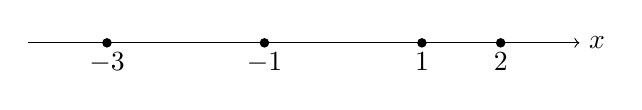
\begin{tikzpicture}
            \draw[->] (-4, 0) -- (3, 0) node[right] {$x$};
            \filldraw (1, 0) circle (\pointSize) node[below] {$1$};
            \filldraw (-1, 0) circle (\pointSize) node[below] {$-1$};
            \filldraw (-3, 0) circle (\pointSize) node[below] {$-3$};
            \filldraw (2, 0) circle (\pointSize) node[below] {$2$};
         \end{tikzpicture}
      }
      \caption{Đồ thị phần 3 bài \ref{intropt}}
      \label{fig:dtp3}
   \end{wrapfigure}
   Kẻ bảng so sánh:
   \begin{table}[h]
      \begin{minipage}{0.48\textwidth}
         \centering
            \begin{tabular}{|c|c|c|c|c|c|c|}
               \hline
               $x$ & $-1$ & $1$ & $-2$ & $2$ & $-3$ & $3$\\
               \hline
               $f(x)$ & $0$ & $0$ & $4$ & $3$ & $7$ & $0$\\
               \hline
               $x^2-1$ & $0$ & $0$ & $3$ & $3$ & $7$ & $7$\\
               \hline
            \end{tabular}
            \caption{Giá trị của $f(x)$ và $x^2-1$ ứng với $x$}
            \label{tab:values3}
      \end{minipage}
   \end{table}

   Nhận thấy rằng $\mathcal{P}$ chỉ đúng khi $x\in \{-1; 1; -3; 2\}$ và chúng ta có đồ thị là hình \ref{fig:dtp3}.
}

\begin{wrapfigure}{R}{0.5\textwidth}
   \centering
   \fbox{
      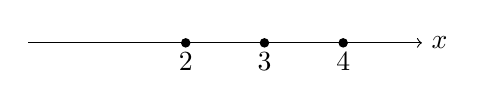
\begin{tikzpicture}
         \draw[->] (0, 0) -- (5, 0) node[right] {$x$};
         \filldraw (2, 0) circle (\pointSize) node[below] {$2$};
         \filldraw (3, 0) circle (\pointSize) node[below] {$3$};
         \filldraw (4, 0) circle (\pointSize) node[below] {$4$};
      \end{tikzpicture}
   }
   \caption{Đồ thị phần 4 bài \ref{intropt}}
   \label{fig:dtp4}
\end{wrapfigure}
4. Nhìn vào bảng được cho, có $f(x) = g(x)$ khi và chỉ khi $x\in \{2; 3; 4\}$. Do đó, đồ thị của $\mathcal{P}$ có được như hình \ref{fig:dtp4}.

5. $\mathcal{P}$ là phương trình có hai ẩn $x$ và $y$, do đó đồ thị của $\mathcal{P}$ là một mặt phẳng hai chiều. Coi như trục hoành biểu diễn cho $x$ và trục tung biểu diễn cho $y$. 

\begin{wraptable}{R}{0.5\textwidth}
   \centering
   \begin{tabular}{|c|c|c|c|c|}
      \hline
      $B_n$ & $3$ & $5$ & $7$ & $11$ \\
      \hline
      $x$ & $2$ & $3$ & $4$ & $5$ \\
      \hline
      $y$ & $2$ & $3$ & $4$ & $6$ \\
      \hline 
   \end{tabular}
   \caption{Giá trị của $x$ và $y$ ứng với $B_n$}
   \label{tab:bn_values}
\end{wraptable}

Để có thể vẽ được đồ thị của $\mathcal{P}$, hiển nhiên nhìn ra được rằng cần phải có những điểm $(x;y)$ để hai giá trị $f(x)$ và $g(y)$ bằng nhau. Và để làm được điều đó, trước hết, chúng ta sẽ tìm xem giá trị bằng nhau của $f(x)$ với $g(y)$ này bằng bao nhiêu. Gọi chung giá trị bằng nhau này là $B_n$. Kẻ lại bảng so sánh thành bảng \ref{tab:bn_values}, với $B_n$ là ra trị đầu ra và $x$, $y$ là giá trị lần lượt đưa vào hai hàm $f$ và $g$ để có giá trị đầu ra đó. Và từ đó, chúng ta có đồ thị của $\mathcal{P}$ là hình \ref{fig:dtp5}.

\begin{figure}[h]
   \centering
   \fbox{
      \begin{tikzpicture}
         \draw[->] (0, 0) -- (3.5, 0) node[right] {$x$};
         \draw[->] (0, 0) -- (0, 3.5) node[above] {$y$};
         \filldraw (1, 1) circle (\pointSize) node[right] {$(2; 2)$};
         \filldraw (1.5, 1.5) circle (\pointSize) node[right] {$(3; 3)$};
         \filldraw (2.5, 3) circle (\pointSize) node[right] {$(5; 6)$};
         \filldraw (2, 2) circle (\pointSize) node[right] {$(4; 4)$};
      \end{tikzpicture}
   }
   \caption{Đồ thị phần 5 bài \ref{intropt}}
   \label{fig:dtp5}
\end{figure}

6. $\mathcal{P}$ là phương trình có hai ẩn $x$ và $b$, do đó đồ thị của $\mathcal{P}$ là một mặt phẳng hai chiều. Coi như trục hoành biểu diễn cho $x$ và trục tung biểu diễn cho $b$.

Giải ngược $b$ từ $f(x)$:
\begin{align*}
   f(x) &= 2b - 1 \\
   \iff b &= \frac{f(x) + 1}{2}.
\end{align*}

Từ đây, chúng ta có thể thêm giá trị của $b$ vào bảng được cho thành bảng \ref{tab:b_values6}

\begin{table}[h]
   \centering
   \begin{tabular}{|c|c|c|c|c|c|c|}
      \hline
      $x$ & $1$ & $2$ & $3$ & $4$ & $5$ & $6$\\
      \hline
      $f(x)$ & $2$ & $3$ & $5$ & $7$ & $11$ & $13$\\
      \hline
      $b$ & $\frac{3}{2}$ & $\frac{5}{2}$ & $3$ & $4$ & $6$ & $7$\\
      \hline
   \end{tabular}
   \caption{Giá trị của $b$ ứng với $x$}
   \label{tab:b_values6}
\end{table}

Qua bảng đó, vẽ được đồ thị của $\mathcal{P}$ như hình \ref{fig:dtp6}.

\begin{figure}[h]
   \centering
   \fbox{
      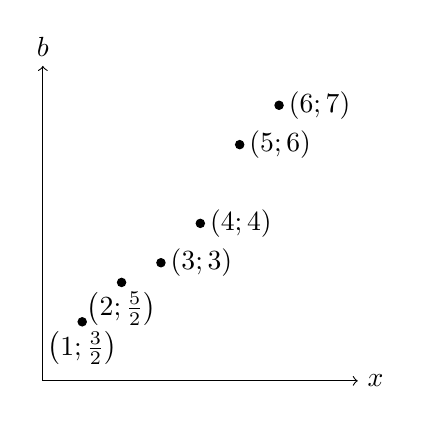
\begin{tikzpicture}
         \draw[->] (0, 0) -- (4, 0) node[right] {$x$};
         \draw[->] (0, 0) -- (0, 4) node[above] {$b$};
         \filldraw (0.5, 0.75) circle (\pointSize) node[below] {$\left(1; \frac{3}{2}\right)$};
         \filldraw (1, 1.25) circle (\pointSize) node[below] {$\left(2; \frac{5}{2}\right)$};
         \filldraw (1.5, 1.5) circle (\pointSize) node[right] {$(3; 3)$};
         \filldraw (2, 2) circle (\pointSize) node[right] {$(4; 4)$};
         \filldraw (2.5, 3) circle (\pointSize) node[right] {$(5; 6)$};
         \filldraw (3, 3.5) circle (\pointSize) node[right] {$(6; 7)$};
      \end{tikzpicture}
   }
   \caption{Đồ thị phần 6 bài \ref{intropt}}
   \label{fig:dtp6}
\end{figure}

7. Nhìn vào bảng, $f(x)$ có thể nhận các giá trị là $\{0; 3; 4; 7\}$.

Khi $f(x) \neq 0$, chỉ có một giá trị đầu vào cho $f$ sao cho $f(x)$ đạt được giá trị đầu ra. Ví dụ, chỉ có đầu vào $x = 2$ mới có $f(x) = 3$. Do đó, khi $f(x) \neq 0$, $x = 2b-1$. Biến đổi đại số cơ bản để có $b = \frac{x + 1}{2}$. Kẻ bảng:

\begin{table}[h]
   \centering
   \begin{tabular}{|c|c|c|c|}
      \hline
      $x$ & $-2$ & $2$ & $-3$\\
      \hline
      $b = \frac{x+1}{2}$ & $-\frac{3}{2}$ & $2$ & $-1$\\
      \hline
   \end{tabular}
   \caption{Giá trị của cặp $(x; b)$ với $f(x) \neq 0$}
   \label{tab:b_values7}
\end{table}

Khi $f(x) = 0$, $x$ và $2b-1$ có thể nhận bất cứ giá trị nào trong tập $\{-1; 1; -3\}$. Từ đó, có thể chọn $x \in \{-1; 1; 3\}$ và giải đại số để chọn $b \in \left\{\frac{-1+1}{2}; \frac{1+1}{2}; \frac{3+1}{2}\right\} = \{0; 1; 2\}$. Các cặp $(x; b)$ thỏa mãn là $(x; b) \in \left\{\left(-1; 0\right); \left(-1; 1\right); \left(-1; 2\right); \left(1; 0\right); \left(1; 1\right); \left(1; 2\right); \left(-3; 0\right); \left(-3; 1\right); \left(-3; 2\right)\right\}$.

Cuối cùng, kết hợp hai trường hợp, chúng ta có đồ thị cho $\mathcal{P}$:

\begin{figure}[H]
   \centering
   \fbox{
      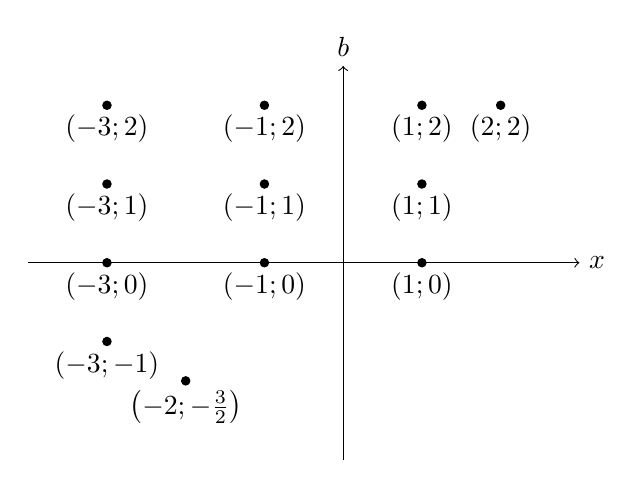
\begin{tikzpicture}
         \draw[->] (-4, 0) -- (3, 0) node[right] {$x$};
         \draw[->] (0, -2.5) -- (0, 2.5) node[above] {$b$};
         
         % Vẽ phần f(x) khác 0
         \filldraw (-2, -1.5) circle (\pointSize) node[below] {$\left(-2; -\frac{3}{2}\right)$};
         \filldraw (2, 2) circle (\pointSize) node[below] {$\left(2; 2\right)$};
         \filldraw (-3, -1) circle (\pointSize) node[below] {$\left(-3; -1\right)$};
         
         \filldraw (-1, 0) circle (\pointSize) node[below] {$\left(-1; 0\right)$};
         \filldraw (1, 0) circle (\pointSize) node[below] {$\left(1; 0\right)$};
         \filldraw (-3, 0) circle (\pointSize) node[below] {$\left(-3; 0\right)$};
         
         \filldraw (-1, 1) circle (\pointSize) node[below] {$\left(-1; 1\right)$};
         \filldraw (1, 1) circle (\pointSize) node[below] {$\left(1; 1\right)$};
         \filldraw (-3, 1) circle (\pointSize) node[below] {$\left(-3; 1\right)$};
         
         \filldraw (-1, 2) circle (\pointSize) node[below] {$\left(-1; 2\right)$};
         \filldraw (1, 2) circle (\pointSize) node[below] {$\left(1; 2\right)$};
         \filldraw (-3, 2) circle (\pointSize) node[below] {$\left(-3; 2\right)$};
      \end{tikzpicture}
   }
   \caption{Đồ thị phần 7 bài \ref{intropt}}
   \label{fig:dtp7}
\end{figure}

8. $\mathcal{P}$ là phương trình có ba ẩn $a$, $b$ và $c$, do đó đồ thị của $\mathcal{P}$ là một mặt phẳng ba chiều. Coi như trục hoành biểu diễn cho $a$, trục tung biểu diễn cho $b$ và trục cao biểu diễn cho $c$.

Theo $\mathcal{P}$, chúng ta cần phải chọn ba số trong tập giá trị của $f$ để hai trong ba số có tổng bằng số còn lại. Từ bảng, nhận thấy rằng, chỉ có thể có hai tổng $4 + 3 = 7$ và $0 + 0 = 0$.

Xét trường hợp đầu tiên, chúng ta có $f(c) = 7$ và $\left(f(a); f(b)\right) \in \left\{\left(4; 3\right); \left(3; 4\right)\right\}$. Tìm ngược lại đầu vào để được $(a; b; c) \in \left\{\left(2; -2; -3\right); \left(-2; 2; -3\right)\right\}$.

Xét trường hợp thứ hai, chúng ta có $f(a) = f(b) = f(c) = 0$. Từ đó, $a$, $b$ và $c$ có thể nhận bất cứ giá trị nào trong tập $\{-3; -1; 1\}$.

Kết hợp hai trường hợp, đồ thị cuối cùng của $\mathcal{P}$ sẽ là hình \ref{fig:dtp8}.

\begin{figure}[H]
   \centering
   \tdplotsetmaincoords{80}{30}
   \fbox{
      \begin{tikzpicture}[tdplot_main_coords]
         \draw[->] (-5, 0, 0) -- (2, 0, 0) node[right] {$a$};
         \draw[->] (0, -5, 0) -- (0, 4, 0) node[above] {$b$};
         \draw[->] (0, 0, -4) -- (0, 0, 2) node[above] {$c$};
         \filldraw (2, -2, -3) circle (\pointSize) node[font=\scriptsize, anchor=north] {$\left(2; -2; -3\right)$};  
         \filldraw (-2, 2, -3) circle (\pointSize) node[font=\scriptsize, anchor=south] {$\left(-2; 2; -3\right)$};  
         \foreach \x/\y/\z in {
            -3/-3/-3, -3/-3/-1, -3/-3/1, 
            -3/-1/-3, -3/-1/-1, -3/-1/1, -3/1/-3, -3/1/-1, -3/1/1,
            -1/-3/-3, -1/-3/-1, -1/-3/1, -1/-1/-3, -1/-1/-1, -1/-1/1,
            -1/1/-3, -1/1/-1, -1/1/1, 1/-3/-3, 1/-3/-1, 1/-3/1,
            1/-1/-3, 1/-1/-1, 1/-1/1, 1/1/-3, 1/1/-1, 1/1/1
         } {
            \filldraw (\x, \y, \z) circle (\pointSize);
            \node[font=\scriptsize, anchor=east] at (\x, \y, \z) {$\left(\x, \y, \z\right)$};
         }
      \end{tikzpicture}
   }
   \caption{Đồ thị phần 8 bài \ref{intropt}}
   \label{fig:dtp8}
\end{figure}

\exercise[ex:hpt1] Vẽ đồ thị của hệ phương trình $\mathcal{P}$, với các định nghĩa đã cho. Hàm có tập xác định là bộ số đầu vào cho ở trong bảng.
\begin{enumerate}
   \item 
   \begin{tabular}{|c|c|c|c|c|c|c|}
      \hline
      $x$ & $0$ & $1$ & $2$ & $3$ & $4$ & $5$ \\
      \hline
      $f(x)$ & $-1$ & $-1$ & $-1$ & $-2$ & $-3$ & $-3$\\
      \hline
   \end{tabular},
   \begin{tabular}{|c|c|c|c|c|c|c|}
      \hline
      $y$ & $0$ & $-2$ & $4$ & $-6$ & $8$ & $-10$\\
      \hline
      $g(y)$ & $-1$ & $-2$ & $-3$ & $-7$ & $-8$ & $-9$\\
      \hline
   \end{tabular},

   \noindent\begin{tabular}{|c|c|c|c|c|c|c|}
      \hline
      $z$ & $-1$ & $1$ & $-2$ & $0$ & $-4$ & $4$\\
      \hline
      $h(z)$ & $2$ & $1$ & $0$ & $-1$ & $-2$ & $-3$\\
      \hline
   \end{tabular} và $\mathcal{P}:f(x) = g(x) = h(x)$;

   \item
   \begin{tabular}{|c|c|c|c|c|c|c|}
      \hline
      $x$ & $0$ & $1$ & $2$ & $3$ & $4$ & $5$ \\
      \hline
      $f(x)$ & $-1$ & $-1$ & $-1$ & $-2$ & $-3$ & $-3$\\
      \hline
   \end{tabular},
   \begin{tabular}{|c|c|c|c|c|c|c|}
      \hline
      $y$ & $0$ & $-2$ & $4$ & $-6$ & $8$ & $-10$\\
      \hline
      $g(y)$ & $-1$ & $-2$ & $-3$ & $-7$ & $-8$ & $-9$\\
      \hline
   \end{tabular},

   \noindent\begin{tabular}{|c|c|c|c|c|c|c|}
      \hline
      $z$ & $-1$ & $1$ & $-2$ & $0$ & $-4$ & $4$\\
      \hline
      $h(z)$ & $2$ & $1$ & $0$ & $-1$ & $-2$ & $-3$\\
      \hline
   \end{tabular} và $\mathcal{P}:f(a) = g(b) = h(c)$;

   \item
   \begin{tabular}{|c|c|c|c|c|c|c|}
      \hline
      $x$ & $0$ & $1$ & $2$ & $3$ & $4$ & $5$ \\
      \hline
      $f(x)$ & $-1$ & $-1$ & $-1$ & $-2$ & $-3$ & $-3$\\
      \hline
   \end{tabular},
   \begin{tabular}{|c|c|c|c|c|c|c|}
      \hline
      $y$ & $0$ & $-2$ & $4$ & $-6$ & $8$ & $-10$\\
      \hline
      $g(y)$ & $-1$ & $-2$ & $-3$ & $-7$ & $-8$ & $-9$\\
      \hline
   \end{tabular},

   \noindent\begin{tabular}{|c|c|c|c|c|c|c|}
      \hline
      $z$ & $-1$ & $1$ & $-2$ & $0$ & $-4$ & $4$\\
      \hline
      $h(z)$ & $2$ & $1$ & $0$ & $-1$ & $-2$ & $-3$\\
      \hline
   \end{tabular} và $\mathcal{P}:\begin{cases}f(o) = g(p)\\f(p + 1) = h(q)\end{cases}$.

   \item
   \begin{tabular}{|c|c|c|c|c|c|c|}
      \hline
      $x$ & $0$ & $1$ & $2$ & $3$ & $4$ & $5$ \\
      \hline
      $f(x)$ & $-1$ & $-1$ & $-1$ & $-2$ & $-3$ & $-3$\\
      \hline
   \end{tabular},
   \begin{tabular}{|c|c|c|c|c|c|c|}
      \hline
      $y$ & $0$ & $-2$ & $4$ & $-6$ & $8$ & $-10$\\
      \hline
      $g(y)$ & $-1$ & $-2$ & $-3$ & $-7$ & $-8$ & $-9$\\
      \hline
   \end{tabular},

   \noindent\begin{tabular}{|c|c|c|c|c|c|c|}
      \hline
      $z$ & $-1$ & $1$ & $-2$ & $0$ & $-4$ & $4$\\
      \hline
      $h(z)$ & $2$ & $1$ & $0$ & $-1$ & $-2$ & $-3$\\
      \hline
   \end{tabular} và $\mathcal{P}:\begin{cases}f(m) = n\\g(n) = h(w)\end{cases}$.
\end{enumerate}

\solution[ex:hpt1]

1. Giá trị đầu vào để $f, g, h$ đều có cùng một đầu ra là $x\in\{0;4\}$. Vậy, chúng ta có đồ thị như hình \ref{fig:hpt11}.

\begin{figure}[H]
   \centering
   \fbox{
      \begin{tikzpicture}
         \draw[->] (-1, 0) -- (5, 0) node[right] {$x$};
         \filldraw (0, 0) circle (\pointSize) node[below] {$0$};
         \filldraw (4, 0) circle (\pointSize) node[below] {$4$};
      \end{tikzpicture}
   }
   \caption{Đồ thị phần 1 bài \ref{ex:hpt1}}
   \label{fig:hpt11}
\end{figure}

2. Trước hết, cần tìm những giá trị chung trong tập giá trị của $f, g, h$. Nhận thấy rằng, có $-1, -2$ và $-3$ là những giá trị chung trong đó. 
\begin{itemize}
   \item Với đầu ra là $-1$, chúng ta có $f(a) = g(b) = h(c) = -1$. Từ đó, chúng ta có $a \in \{0; 1; 2\}$ và $b = c = 0$.
   \item Trong trường hợp kết quả của hàm là $-2$, $f(a) = g(b) = h(c) = -2$. Từ đó, bộ ba $\left(a; b; c\right)$ có giá trị là $(3; -2; -4)$.
   \item Trong trường hợp kết quả của hàm là $-3$, $f(a) = g(b) = h(c) = -3$. Từ đó, $\left(a; b; c\right)$ $\in \left\{\left(4; 4; 4\right); \left(5; 4; 4\right)\right\}$.
\end{itemize}
Kết hợp ba trường hợp, xây dựng không gian tọa độ, chúng ta có hình \ref{fig:hpt12}.

\begin{figure}[H]
   \centering
   \fbox{
      \tdplotsetmaincoords{80}{-10}
      \begin{tikzpicture}[tdplot_main_coords]
         \draw[->] (-3, 0, 0) -- (6, 0, 0) node[right] {$a$};
         \draw[->] (0, -2, 0) -- (0, 5, 0) node[above] {$b$};
         \draw[->] (0, 0, -5) -- (0, 0, 5) node[above] {$c$};
         \filldraw (0, 0, 0) circle (\pointSize) node[below left] {$\left(0; 0; 0\right)$};
         \filldraw (1, 0, 0) circle (\pointSize) node[above] {$\left(1; 0; 0\right)$};
         \filldraw (2, 0, 0) circle (\pointSize) node[below] {$\left(2; 0; 0\right)$};
         \filldraw (3, -2, -4) circle (\pointSize) node[above] {$\left(3; -2; -4\right)$};
         \filldraw (4, 4, 4) circle (\pointSize) node[above] {$\left(4; 4; 4\right)$};
         \filldraw (5, 4, 4) circle (\pointSize) node[below] {$\left(5; 4; 4\right)$};
      \end{tikzpicture}
   }
   \caption{Đồ thị phần 2 bài \ref{ex:hpt1}}
   \label{fig:hpt12}
\end{figure}

3. Để $f$ và $g$ nhận cùng một giá trị thì giá trị đầu ra đó, theo bảng, phải là $-1$, $-2$ hoặc $-3$.
\begin{itemize}
   \item Tại $f(o) = g(p) = -1$, $o \in \{0; 1; 2\}$ và $p = 0$. Từ đó, $f(p + 1) = f(1) = -1$. Khi này, $h(q) = -1 \iff q = 0$.
   \item Tại $f(o) = g(p) = -2$, sau khi tra bảng, chúng ta thấy được rằng $\begin{cases}o = 3\\p = -2\end{cases}$; suy ra $f(p + 1) = f(-1)$, Tuy nhiên, $-1$ không thuộc tập xác định của $f$. Vậy, chúng ta sẽ loại trường hợp này.
   \item Tại $f(o) = g(p) = -3$, $o \in \{4; 5\}$ và $p = 4$. Từ đó, $f(p + 1) = f(5) = -3$. Khi này, $h(q) = -3 \iff q = 4$.
\end{itemize}
Cuối cùng, vẽ đồ thị để được hình \ref{fig:hpt13}.

\begin{figure}[H]
   \tdplotsetmaincoords{80}{-10}
   \centering
   \fbox{
      \begin{tikzpicture}[tdplot_main_coords]
         \draw[->] (-2, 0, 0) -- (6, 0, 0) node[right] {$o$};
         \draw[->] (0, -2, 0) -- (0, 5, 0) node[above] {$p$};
         \draw[->] (0, 0, -2) -- (0, 0, 5) node[above] {$q$};
         \filldraw (0, 0, 0) circle (\pointSize) node[below left] {$\left(0; 0; 0\right)$};
         \filldraw (1, 0, 0) circle (\pointSize) node[above] {$\left(1; 0; 0\right)$};
         \filldraw (2, 0, 0) circle (\pointSize) node[below] {$\left(2; 0; 0\right)$};
         \filldraw (4, 4, 4) circle (\pointSize) node[above] {$\left(4; 4; 4\right)$};
         \filldraw (5, 4, 4) circle (\pointSize) node[below] {$\left(5; 4; 4\right)$};
      \end{tikzpicture}
   }
   \caption{Đồ thị phần 3 bài \ref{ex:hpt1}}
   \label{fig:hpt13}
\end{figure}

4. Theo đề, chúng ta cần tìm những bộ $(m;n;w)$ thỏa mãn $\mathcal{P}$, trong đó có $g(n) = h(w)$. Cho nên, $n$ phải thuộc tập xác định của $g$. Nhìn vào bảng, tập xác định đó là $\{0; -2; 4; -6; 8; -10\}$. Tuy nhiên, cũng có $f(m) = n$, cho nên $n$ vừa phải thuộc tập giá trị của $f$, hay $n \in \{-1; -2; -3\}$. Lấy giao của hai tập đó, chúng ta có $n = -2$. Từ đó, giải $f(m) = -2$ để có $m = 3$. Thêm vào đó, $h(w) = g(-2) = -2 \iff w = -4$.

Bộ số duy nhất thỏa mãn hệ phương trình $\mathcal{P}$ là $\left(m; n; w\right) = \left(3; -2; -4\right)$. Đồ thị của $\mathcal{P}$ là hình \ref{fig:hpt14}.

\begin{figure}[H]
   \tdplotsetmaincoords{80}{20}
   \centering
   \fbox{
      \begin{tikzpicture}[tdplot_main_coords]
         \draw[->] (-1, 0, 0) -- (4, 0, 0) node[right] {$m$};
         \draw[->] (0, -3, 0) -- (0, 1, 0) node[above] {$n$};
         \draw[->] (0, 0, -5) -- (0, 0, 1) node[above] {$w$};
         \filldraw (3, -2, -4) circle (\pointSize ) node[above] {$\left(3; -2; -4\right)$};
      \end{tikzpicture}
   }
   \caption{Đồ thị phần 4 bài \ref{ex:hpt1}}
   \label{fig:hpt14}
\end{figure}
% \subsection{Kí hiệu tổng và tích của nhiều số}

\ % Lùi đầu dòng

Cho hàm số $f(x)$. Khi cho $x$ là số nguyên chạy từ $a$ đến $b$ (thông thường $a \le b$), chúng ta có tổng của các giá trị $f(x)$ được viết rút gọn là
$$
\defMath{\sum_{x=a}^{b} \left(f(x)\right) = f(a) + f(a + 1) + \cdots + f(b)}.
$$

Ví dụ, nếu cho $f(x) = 3x - 7$, thì
\begin{align*}
   \sum_{x = -1}^3 \left(f(x)\right) &= f(-1) + f(0) + f(1) + f(2) + f(3) \\
   &= \left(3(-1) - 7\right) + \left(3(0) - 7\right) + \left(3(1) - 7\right) + \left(3(2) - 7\right) + \left(3(3) - 7\right) \\
   &= -20.
\end{align*}

Đối với tích của các giá trị $f(x)$, chúng ta có
$$
\defMath{\prod_{x=a}^{b} \left(f(x)\right) = f(a) \times f(a + 1) \times \cdots \times f(b)}.
$$

Ví dụ, cùng với $f(x) = 3x - 7$, chúng ta có
\begin{align*}
   \prod_{x = -1}^3 \left(f(x)\right) &= f(-1) \times f(0) \times f(1) \times f(2) \times f(3) \\
   &= \left(3(-1) - 7\right) \times \left(3(0) - 7\right) \times \left(3(1) - 7\right) \times \left(3(2) - 7\right) \times \left(3(3) - 7\right) \\
   &= 560.
\end{align*}

Mở rộng kí hiệu, nếu chúng ta có cần tính tổng hay tích vào hàm phụ thuộc vào các giá trị $x$ thỏa mãn điều kiện $P$ nào đó, thì chúng ta có thể viết
$$
\defMath{\sum_{P} \left(f(x)\right) \text{ và }\prod_{P} \left(f(x)\right)}.
$$

$P$ có thể được viết theo nhiều kiểu khác nhau, miễn hiểu là được. Ví dụ, thay vì tính tổng và tích của $f(x)$ khi $x$ thay đổi từ $-1$ đến $3$, chúng ta có thể tính tổng và tích của $f(x)$ với $x$ là các số nguyên tố lớn hơn $10$ và nhỏ hơn $20$. Khi đó,

{
   \begin{minipageindent}{0.48\textwidth}
      \begin{align*}
         &\sum\limits_{x \text{ là số nguyên tố lớn hơn } 10 \text{ và nhỏ hơn } 20} \left(f(x)\right) \\
         = &f(11) + f(13) + f(17) + f(19) \\
         = &152\text{, và}
      \end{align*}
   \end{minipageindent}
   \hfill
   \begin{minipageindent}{0.48\textwidth}
      \begin{align*}
         &\prod\limits_{x \text{ là số nguyên tố lớn hơn } 10 \text{ và nhỏ hơn } 20} \left(f(x)\right) \\
         = &f(11) \times f(13) \times f(17) \times f(19) \\
         = &1830400.
      \end{align*}
   \end{minipageindent}
}

% \subsection{Hàm đa thức}

\ % Lùi đầu dòng

Hàm \defText{đa thức} thông thường được biểu diễn dưới dạng tổng của các đơn thức $$\defMath{f(x)=P_n(x)=\sum_{i = 0}^n \left(a_i x^i\right) = a_nx^n + a_{n-1}x^{n-1} + \cdots + a_1x + a_0}$$ với $n$ là một số nguyên không âm, $a_i$ là các số thực, gọi là các \defText{hệ số}, với mọi $i$ nguyên nằm trong đoạn $[0, n]$ và $a_n \neq 0$. Khi này, $n$ được gọi là \defText{bậc} của đa thức\label{def:ham_so_mot_bien:da_thuc:da_thuc}. Mọi giá trị $x \in \mathbb{R}$ đều thuộc tập xác định của hàm đa thức $f(x)$. Ví dụ:
\begin{itemize}
   \item $f(x) = 2x^2 + 3x + 1$ là một đa thức bậc $2$ với các hệ số $a_2 = 2$, $a_1 = 3$, $a_0 = 1$;
   \item $g(y) = y^3 - 4y$ là một đa thức bậc $3$ với các hệ số $b_3 = 1$, $b_2 = 0$, $b_1 = -4$, $b_0 = 0$;
   \item $h(z) = 5$ là một đa thức bậc $0$ với hệ số $c_0 = 5$;
\end{itemize}
Tính toán một số giá trị mẫu:
\begin{itemize}
   \item $p(1) = 7 \cdot 1^4 - 2 \cdot 1^2 + 9 = 14$ với $q(t)= 7t^4 - 2t^2 + 9$ là một đa thức bậc $4$ với các hệ số $d_4 = 7$, $d_3 = 0$, $d_2 = -2$, $d_1 = 0$, $d_0 = 9$;
   \item $q(2) = -3 \cdot 2 + 8 = 2$ với $q(r) = -3r + 8$ là một đa thức bậc $1$ với các hệ số $e_1 = -3$, $e_0 = 8$.
\end{itemize}
Khi đa thức có bậc bằng $0$, hay $f = P_0 = a_0$, thì được gọi là \defText{đa thức hằng} hay \defText{hàm hằng}. Một trường hợp đặc biệt là khi $f = 0$ (hay $f(x) = 0$ với mọi $x$). Nếu hàm này là đa thức, theo định nghĩa, hàm này chỉ có duy nhất hệ số đầu $a_0 = 0$. Tuy nhiên, cũng theo định nghĩa thì hệ số đầu phải khác $0$. Vì vậy, hàm không có bậc và không được gọi là đa thức. Nhưng, do hàm nhận giá trị cố định với mọi $x$ nên vẫn được gọi là hàm hằng \footnote{Đa số những nhà toán học không coi $f = 0$ là đa thức bậc $0$ do nhiều tính chất của đa thức bị phá vỡ khi gặp trường hợp này. Tuy nhiên, nhiều người vẫn coi $f = 0$ là đa thức không có bậc. Trong tài liệu này, tác giả không coi $0$ là đa thức, nhưng vẫn coi là hàm hằng.}.

\exercise Phác thảo đồ thị của những hàm sau:
\begin{multicols}{2}
   \begin{enumerate}
      \item $f(x) = x + 2$; 
      \item $f(x) = x^2 + 2x + 3$;
      \item $f(x) = -2x^2 + 5x - 6$;
      \item $f(x) = x^3 - 9x^2 + 24x - 16$;
      \item $f(x) = 2$;
      \item $f(x) = 36x^4 + 28x^3 - 3x^2 - 6x - 1$;
      \item $f(x) = -x^6 + x^2 - 4x - 2$;
      \item $f(x) = -x^7 + x$.
   \end{enumerate}
\end{multicols}

\solution

Bạn đọc có thể dùng những phần mềm vẽ đồ thị để nhanh chóng có hình vẽ. Tuy nhiên, nếu không có thiết bị điện tử thì bạn đọc vẫn có thể vẽ đồ thị bằng giấy và bút bằng cách lấy nhiều điểm ví dụ cho $x$ và tính toán giá trị $f(x)$ và sau đó nối chúng lại với nhau.

Bạn đọc có thể để ý rằng là không phải lúc nào cũng đặt gốc tọa độ ở vị trí chính giữa và tỉ lệ xích trên hai trục không phải là giống nhau. Trong nhiều trường hợp, việc ép đặt gốc ở giữa và giữ tỉ lệ giống nhau trên các trục sẽ làm cho đồ thị lệch ra khỏi khu vực vẽ. Điều quan trọng nhất của những bài vẽ đồ thị trong vật lí không chỉ là căn ke chính xác vị trí từng điểm, mà còn là nhận ra được dáng điệu của đồ thị và vị trí tương đối giữa các điểm trên đồ thị đó. Qua đó, chúng ta rút ra được những tính chất toán học cần thiết để phục vụ những yêu cầu cụ thể trong bài tập ứng dụng.

Dưới đây là đồ thị của các hàm đa thức trong bài:

{
   \begin{minipageindent}{0.48\textwidth}
      \begin{figure}[H]
         \centering
         \begin{tikzpicture}
            \draw[->] (-5, 0) -- (1, 0) node[right] {$x$};
            \draw[->] (0, -3) -- (0, 3) node[above] {$f(x)$};
            \draw[graph thickness, color=colorEmphasisCyan] plot[domain=-5:1] (\x, {\x + 2});
            \filldraw[color=colorEmphasisCyan] (0, 2) circle (\pointSize) node[below right] {$\left(0; 2\right)$};
            \filldraw[color=colorEmphasisCyan] (-2, 0) circle (\pointSize) node[below right] {$\left(-2; 0\right)$};
         \end{tikzpicture}
         \caption{Đồ thị của hàm $f(x) = x + 2$}
         \label{fig:ham_so:ham_da_thuc:x_2}
      \end{figure}
   \end{minipageindent}
   \hfill
   \begin{minipageindent}{0.48\textwidth}
      \begin{figure}[H]
         \centering
         \begin{tikzpicture}
            \draw[->] (-4, 0) -- (2, 0) node[right] {$x$};
            \draw[->] (0, 0) -- (0, 6) node[above] {$f(x)$};
            \draw[color=colorEmphasisCyan, graph thickness, smooth, samples=100] plot[domain=-3:1] (\x, {(\x + 1)^2 + 2});
            \filldraw[color=colorEmphasisCyan] (-1, 2) circle (\pointSize) node[below] {$\left(-1; 2\right)$};
            \filldraw[color=colorEmphasisCyan] (0, 3) circle (\pointSize) node[below right] {$\left(0; 3\right)$};
            \filldraw[color=colorEmphasisCyan] (-2, 3) circle (\pointSize) node[left] {$\left(-2; 3\right)$};
         \end{tikzpicture}
         \caption{Đồ thị của hàm $f(x) = x^2 + 2x + 3$}
         \label{fig:ham_so_mot_bien:da_thuc:x2_2x_3}
      \end{figure}
   \end{minipageindent}
}

{
   \begin{minipageindent}{0.48\textwidth}
      \begin{figure}[H]
         \centering
         \begin{tikzpicture}
            \draw[->] (-2, 0) -- (4, 0) node[right] {$x$};
            \draw[->] (0, -5) -- (0, 1) node[above] {$f(x)$};
            \draw[color=colorEmphasisCyan, graph thickness, smooth, samples=100] plot[domain=-0.186:2.686] (\x, {(-2*(\x)^2 + 5*(\x) - 4)});
            \draw[snake it, name path=A] (-2, -0.25) -- (4, -0.25);
            \draw[snake it, name path=B] (-2, -0.35) -- (4, -0.35);
            \tikzfillbetween[of=A and B]{white};
            \foreach \x/\y/\yy/\pos in {0/-4/-6/right, 1/-1/-3/above, 2/-2/-4/right} {
               \filldraw[color=colorEmphasisCyan] (\x, \y) circle (\pointSize) node[\pos] {$\left(\x; {\yy}\right)$};
            }
         \end{tikzpicture}
         \caption{Đồ thị của hàm $f(x) = -2x^2 + 5x - 6$}
         \label{fig:ham_so_mot_bien:da_thuc:t2x2_5x_t6}
      \end{figure}
   \end{minipageindent}
   \hfill
   \begin{minipageindent}{0.48\textwidth}
      \begin{figure}[H]
         \centering
         \begin{tikzpicture}
            \draw[->] (0, 0) -- (6, 0) node[right] {$x$};
            \draw[->] (0, -3) -- (0, 5) node[above] {$f(x)$};
            \draw[color=colorEmphasisCyan, graph thickness, smooth, samples=100] plot[domain=0.508:5.492] (\x, {((\x)^3 - 9*(\x)^2 + 24*(\x) - 16) / 2});
            \filldraw[color=colorEmphasisCyan] (2, 2) circle (\pointSize) node[above] {$\left(2; 4\right)$};
            \filldraw[color=colorEmphasisCyan] (4, 0) circle (\pointSize) node[below] {$\left(4; 0\right)$};
            \filldraw[color=colorEmphasisCyan] (1, 0) circle (\pointSize) node[below right] {$\left(1; 0\right)$};
            \filldraw[color=colorEmphasisCyan] (5, 2) circle (\pointSize) node[right] {$\left(5; 4\right)$};
         \end{tikzpicture}
         \caption{Đồ thị của hàm $f(x) = x^3 - 9x^2 + 24x - 16$}
         \label{fig:ham_so_mot_bien:da_thuc:x3_t9x2_24x_t16}
      \end{figure}
   \end{minipageindent}
}

Ở hình \ref{fig:ham_so_mot_bien:da_thuc:t2x2_5x_t6}, đồ thị có đoạn díc dắc. Ý nghĩa của cách vẽ này là để cắt bỏ phần đồ thị không cần thiết.

{
   \begin{minipageindent}{0.48\textwidth}
      \begin{figure}[H]
         \centering
         \begin{tikzpicture}
            \draw[->] (-3, 0) -- (3, 0) node[right] {$x$};
            \draw[->] (0, -1) -- (0, 3) node[above] {$f(x)$};
            \draw[graph thickness, color=colorEmphasisCyan] plot[domain=-3:3] (\x, {2});
            \filldraw[color=colorEmphasisCyan] (0, 2) circle (\pointSize) node[above left] {$\left(0; 2\right)$};
         \end{tikzpicture}
         \caption{Đồ thị của hàm $f(x) = 2$}
         \label{fig:ham_so:ham_da_thuc:2}
      \end{figure}
   \end{minipageindent}
   \hfill
   \begin{minipageindent}{0.48\textwidth}
      \begin{figure}[H]
         \centering
         \begin{tikzpicture}
            \draw[->] (-3, 0) -- (3, 0) node[right] {$x$};
            \draw[->] (0, -3) -- (0, 3) node[above] {$f(x)$};
            \draw[color=colorEmphasisCyan, graph thickness, smooth, samples=100] plot[domain=-2.491:1.669] (\x, {36*(\x/3)^4 + 28*(\x/3)^3 - 3*(\x/3)^2 - 6*(\x/3) - 1});
            \foreach \x/\y/\xlabel/\ylabel/\pos in {
               -1.5/0/{-0,5}/0/below,
               -0.721/0/{-0,24}/0/above,
               0/-1/0/-1/left,
               0.75/-2.109/{0,25}/{-2,11}/below,
               1.387/0/{0,462}/0/below right,
               -2.357/2/{-0,79}/2/right,
               1.5/1/{0,5}/1/right} {
               \filldraw[color=colorEmphasisCyan] (\x, \y) circle (\pointSize) node[\pos] {$\left(\xlabel;\ylabel\right)$};
            }
         \end{tikzpicture}
         \caption{Đồ thị của hàm $f(x) = 36x^4 + 28x^3 - 3x^2 - 6x - 1$}
         \label{fig:ham_so:ham_da_thuc:36x4_28x3_t3x2_t6x_t1}
      \end{figure}
   \end{minipageindent}
}

{
   \begin{minipageindent}{0.48\textwidth}
      \begin{figure}[H]
         \centering
         \begin{tikzpicture}
            \draw[->] (-3, 0) -- (3, 0) node[right] {$x$};
            \draw[->] (0, -4) -- (0, 2) node[above] {$f(x)$};
            \draw[color=colorEmphasisCyan, graph thickness, smooth, samples=80] plot[domain=-3:2.356] (\x, {(-(\x / 2)^6 + (\x / 2)^2 - 2*(\x) - 2)/2});
            \foreach \x/\y/\xlabel/\ylabel/\pos in {
               -3/-2.570/{-1,5}/{-5,14}/right,
               -2/1/-1/2/above,
               0/-1/0/-1/below left,
               2.356/-4/{1,18}/-8/left} {
               \filldraw[color=colorEmphasisCyan] (\x, \y) circle (\pointSize) node[\pos] {$\left(\xlabel;\ylabel\right)$};
            }
         \end{tikzpicture}
         \caption{Đồ thị của hàm $f(x) = -x^6 + x^2 - 4x - 2$}
         \label{fig:ham_so:ham_da_thuc:tx6_x2_t4x_t2}
      \end{figure}
   \end{minipageindent}
   \hfill
   \begin{minipageindent}{0.48\textwidth}
      \begin{figure}[H]
         \centering
         \begin{tikzpicture}
            \draw[->] (-3, 0) -- (3, 0) node[right] {$x$};
            \draw[->] (0, -3) -- (0, 3) node[above] {$f(x)$};
            \draw[color=colorEmphasisCyan, graph thickness, smooth, samples=80] plot[domain=-1.229:1.229] (\x, {-(\x)^7 + (\x)});
            \foreach \x/\y/\xlabel/\ylabel/\pos in {
               -1/0/-1/0/above left,
               0/0/0/0/below right,
               1/0/1/0/above right,
               0.723/0.62/{0,72}/{0,62}/above,
               -0.723/-0.62/{-0,72}/{-0,62}/below left}{
                  \filldraw[color=colorEmphasisCyan] (\x, \y) circle (\pointSize) node[\pos] {$\left(\xlabel;\ylabel\right)$};
            }
         \end{tikzpicture}
         \caption{Đồ thị của hàm $f(x) = -x^7 + x$}
         \label{fig:ham_so:ham_da_thuc:tx7_x}
      \end{figure}
   \end{minipageindent}
}

\exercise Giải những phương trình sau. Các phương trình đều có ẩn là $x \in \mathbb{R}$.
\begin{multicols}{2}
   \begin{enumerate}
      \item $3x - 7 = 0$;
      \item $x - 9 = 5x + 3$;
      \item $\frac{1}{v}\cdot x - \frac{1}{v} \cdot x_0 = t$, với $v$, $x_0$, $t$ là những tham số thực;
      \item $6x^2 - 5x - 21 = 0$;
      \item $5x^2 - 50x + 125 = 0$;
      \item $x^2 + 2x + 4 = 0$;
      \item $x^2 + 2x + 4 = 8$;
      \item $5x^2 - 20x + 20 = x^2 - 4$;
      \item $\frac{1}{2}kx^2 + \frac{1}{2}mv^2 = \frac{1}{2}kx_0^2$, với $k$, $m$, $v$, $x_0$ là những tham số thực;
      \item $x^3 - \frac{11}{6}\cdot x^2 + x - \frac{1}{6} = 0$;
      \item $2x^3 - 2x^2 + 2x - 2 = 6 + 6x^2$;
      \item $x^4+2x^3-x^2-2x=0$;
      \item $-x^4 -3x^2 = -5$;
      \item $x^4 + 1 = 3x^3 + x^2 + 3x$.
   \end{enumerate}
\end{multicols}

\solution

\setcounter{subexercise}{1}
\arabic{subexercise}. Biến đổi tương đương phương trình để có:
\begin{align*}
   3x - 7 &= 0 \\
   \iff 3x &= 7\\
   \iff x &= \frac{7}{3}.
\end{align*}
Vậy tập nghiệm của phương trình là $\displaystyle\left\{\frac{7}{3}\right\}$.

\stepcounter{subexercise}
\arabic{subexercise}. Chuyển số hạng có thừa số $x$ về một phía, và số hạng tự do về phía còn lại để được:
\begin{align*}
   x - 9 &= 5x + 3 \\
   \iff (x - 9) + (9 - 5x) &= (5x + 3) + (9 - 5x) \\ 
   \iff -4x &= 12 \\
   \iff x &= -3.
\end{align*}
Vậy tập nghiệm của phương trình là $\displaystyle\left\{-3\right\}$.

\stepcounter{subexercise}
\arabic{subexercise}. Để giải phương trình có chứa tham số, chúng ta cần viết lại ẩn $x$ dưới dạng một biểu thức chỉ chứa tham số và hằng số. Cụ thể,
\begin{align*}
   \frac{1}{v}\cdot x - \frac{1}{v} \cdot x_0 &= t \\
   \iff \frac{x}{v} &= t + \frac{x_0}{v} \\
   \iff x &= vt + x_0.
\end{align*}
Vậy nghiệm của phương trình là $\displaystyle\left\{vt + x_0\right\}$.

\stepcounter{subexercise}
\arabic{subexercise}. Nếu như bạn đọc chưa biết, nếu như một đa thức $f(x)$ nhận $x = a$ là nghiệm thì $f(x)$ có thể được viết thành tích của $(x - a)$ nhân một đa thức $g(x)$ với bậc nhỏ hơn $1$ so với $f(x)$. Và nếu $g(x)$ lại có nghiệm $x = b$ thì chúng ta có thể viết $g(x) = (x-b)h(x)$ và qua đó có thể viết lại $f(x) = (x-a)(x-b)h(x)$. Một cách tổng quát nhất, nếu như $f(x)$ là phương trình bậc $n$ có $n$ nghiệm $a_1, a_2, \cdots, a_n$ thì có thể viết lại $$f(x) = A \prod_{i=1}^{n} (x - a_i) = A(x - a_1)(x - a_2)\cdots (x - a_n)$$ với $A$ là hệ số của số hạng có bậc lớn nhất trong đa thức $f(x)$.

Nhẩm nghiệm (bằng cách bấm máy tính) phương trình thì có $x = -\frac{3}{2}$ và $x = \frac{7}{3}$. Chúng ta kì vọng có thể viết lại phương trình dưới dạng $6\left(x - \left(-\frac{3}{2}\right)\right)\left(x - \frac{7}{3}\right) = 0$. Thực vậy, thực hiện phân tích nhân tử để có:
\begin{align*}
   &6x^2 - 5x - 21 = 0 \\
   \iff &6x^2 - 14x + 9x - 21 = 0 \\
   \iff &2x(3x - 7) + 3(3x - 7) = 0 \\
   \iff &(2x + 3)(3x - 7) = 0 \\
   \iff &\left[
      \begin{aligned}
         2x + 3 &= 0 \\
         3x - 7 &= 0
      \end{aligned}
   \right.
   \iff \left[
      \begin{aligned}
         x &= -\frac{3}{2} \\
         x &= \frac{7}{3}
      \end{aligned}
   \right..
\end{align*}
Vậy phương trình có nghiệm là $\displaystyle\left\{-\frac{3}{2}; \frac{7}{3}\right\}$.

\stepcounter{subexercise}
\arabic{subexercise}.
\begin{align*}
   5x^2 - 50x + 125 &= 0 \\
   \iff 5\left(x^2 - 10x + 25\right) &= 0 \\
   \iff 5(x - 5)^2 &= 0 \\
   \iff x - 5 &= 0 \\
   \iff x &= 5.
\end{align*}

Vậy tập nghiệm của phương trình có một phần tử duy nhất $\displaystyle\left\{5\right\}$.

\stepcounter{subexercise}
\arabic{subexercise}. Với những phương trình liên quan tới đa thức bậc hai không thể nhẩm ngay được nghiệm, chúng ta sẽ sử dụng phương pháp tách bình phương. Với phương trình được cho:
\begin{align}
   x^2 + 2x + 4 &= 0 \nonumber\\ 
   \iff x^2 + 2x + 1 &= -3 \nonumber\\
   \iff (x + 1)^2 &= -3. \label{eq:ham_so_mot_bien:ham_da_thuc:gptdt6}
\end{align}
Một số thực nhân với chính nó sẽ ra một số không âm. Cho nên phương trình \ref{eq:ham_so_mot_bien:ham_da_thuc:gptdt6} không thể đúng. Vậy phương trình vô nghiệm trên tập số thực.

\stepcounter{subexercise}
\arabic{subexercise}. 
\begin{align*}
   &x^2 + 2x + 4 = 8 \\ 
   \iff &x^2 + 2x + 1 = 5 \\
   \iff &(x + 1)^2 = 5 \\
   \iff &\left[
      \begin{aligned}
         x + 1 &= \sqrt{5} \\
         x + 1 &= -\sqrt{5}
      \end{aligned}
   \right. \\
   \iff &\left[
      \begin{aligned}
         x &= \sqrt{5} - 1 \\
         x &= -\sqrt{5} - 1
      \end{aligned}
   \right..
\end{align*}
Vậy tập nghiệm của phương trình là $\displaystyle\left\{\sqrt{5} - 1; -\sqrt{5} - 1\right\}$.

\stepcounter{subexercise}
\arabic{subexercise}. Phần này tác giả làm khác so với phần 2. Chuyển đổi toàn bộ phương trình về một vế để đưa về dạng phương trình $f(x) = 0$:
\begin{align*}
   &5x^2 - 20x + 20 = x^2 - 4 \\
   \iff &4x^2 - 20x + 24 = 0 \\
   \iff &4\left(x^2 - 5x + 6\right) = 0 \\
   \iff &4\left(x^2 - 2x - 3x + 6\right) = 0 \\
   \iff &4\left(x(x - 2) - 3(x - 2)\right) = 0 \\
   \iff &4(x - 3)(x - 2) = 0 \\
   \iff &\left[
      \begin{aligned}
         x - 3 &= 0 \\
         x - 2 &= 0
      \end{aligned}
   \right. \iff x \in \left\{3; 2\right\}. 
\end{align*}
Vậy phương trình có tập nghiệm $\left\{3; 2\right\}$.

\stepcounter{subexercise}
\arabic{subexercise}. Nhân cả hai vế với $2$ để khử phân số trong phương trình:
\begin{align}
   &\frac{1}{2}kx^2 + \frac{1}{2}mv^2 = \frac{1}{2}kx_0^2 \nonumber \\
   \iff &kx^2 + mv^2 = kx_0^2. \label{eq:ham_so_mot_bien:ham_da_thuc:gptdt9}
\end{align}
Xong, thực hiện chuyển vế để giữ thừa số chứa $x^2$ ở một bên, phương trình \ref{eq:ham_so_mot_bien:ham_da_thuc:gptdt9} tương đương với
\begin{align*}
   (\ref{eq:ham_so_mot_bien:ham_da_thuc:gptdt9}) \iff &kx^2 = kx_0^2 - mv^2 \\
   \iff & x^2 = x_0^2 - \frac{mv^2}{k}.
\end{align*}

Với trường hợp $x_0^2 - \frac{mv^2}{k} < 0$ thì phương trình vô nghiệm do $x^2$ không thể âm. Trong trường hợp còn lại, lấy căn bậc hai hai vế để có $$x\in\left\{\sqrt{x_0^2 - \frac{mv^2}{k}}; -\sqrt{x_0^2 - \frac{mv^2}{k}}\right\}.$$ Tại giá trị đặc biệt mà khi $x_0^2 = \frac{mv^2}{k}$ thì tập nghiệm suy biến thành $\left\{0\right\}$.

Vậy, phương trình có nghiệm là 
$$
\begin{cases}
   \left\{\sqrt{x_0^2 - \frac{mv^2}{k}}; -\sqrt{x_0^2 - \frac{mv^2}{k}}\right\} &\text{ nếu } x_0^2 - \frac{mv^2}{k} \geq 0 \\
   \emptyset &\text{ nếu } x_0^2 - \frac{mv^2}{k} < 0
\end{cases}.
$$

\stepcounter{subexercise}
\arabic{subexercise}. Phân tích thừa số với để ý rằng $1$, $\frac{1}{2}$ và $\frac{1}{3}$ là nghiệm:
\begin{align*}
   &x^3 - \frac{11}{6}\cdot x^2 + x - \frac{1}{6} = 0 \\
   \iff &x^3 - x^2 - \frac{5}{6}x^2 + \frac{5}{6}x + \frac{1}{6}x - \frac{1}{6} = 0 \\
   \iff &x^2\left(x - 1\right) - \frac{5}{6}x\left(x - 1\right) + \frac{1}{6}\left(x - 1\right) = 0 \\
   \iff &\left(x - 1\right)\left(x^2 - \frac{5}{6}x + \frac{1}{6}\right) = 0 \\
   \iff &\left(x - 1\right)\left(x^2 - \frac{1}{2}x - \frac{1}{3}x + \frac{1}{6}\right) = 0 \\
   \iff &\left(x - 1\right)\left(x\left(x - \frac{1}{2}\right) - \frac{1}{3}\left(x - \frac{1}{2}\right)\right) = 0 \\
   \iff &\left(x - 1\right)\left(x - \frac{1}{2}\right)\left(x - \frac{1}{3}\right) = 0
\end{align*}
\begin{align*}
   \iff &\left[
      \begin{aligned}
         x - 1 &= 0 \\
         x - \frac{1}{2} &= 0 \\
         x - \frac{1}{3} &= 0
      \end{aligned}
   \right. \\
   \iff &\left[
      \begin{aligned}
         x &= 1 \\
         x &= \frac{1}{2} \\
         x &= \frac{1}{3}
      \end{aligned}
   \right..
\end{align*}
Cuối cùng, như chúng ta đã dự đoán, phương trình có nghiệm là $\displaystyle\left\{1; \frac{1}{2}; \frac{1}{3}\right\}$.

\stepcounter{subexercise}
\arabic{subexercise}. Có một cách là chuyển phương trình về một vế rồi nhẩm nghiệm. Dưới đây, tác giả sẽ trình bày một góc nhìn khác để giải bài toán này.
\begin{align}
   2x^3 - 2x^2 + 2x - 2 &= 6 + 6x^2 \nonumber\\
   \iff \left(2x^3 + 2x\right) - \left(2x^2 + 2\right) &= 6x^2 + 6 \nonumber\\
   \iff 2x\left(x^2 + 1\right) - 2\left(x^2 + 1\right) &= 6\left(x^2 + 1\right) \nonumber\\
   \iff \left(2x - 2\right)\left(x^2 + 1\right) &= 6\left(x^2 + 1\right). \label{eq:ham_so_mot_bien:ham_da_thuc:gptdt11}
\end{align}
Để ý rằng, do $x^2 \geq 0$ nên $x^2 + 1 \geq 1 > 0$. Chúng ta đã chỉ ra rằng $x^2 + 1 \neq 0$, và qua đó, chúng ta có thể an toàn chia hai vế của \ref{eq:ham_so_mot_bien:ham_da_thuc:gptdt11} cho $x^2 + 1$ để có:
\begin{align*}
   2x - 2 &= 6 \\
   \iff x &= 4.
\end{align*}
Vậy phương trình có nghiệm là $\displaystyle\left\{4\right\}$.

\stepcounter{subexercise}
\arabic{subexercise}. Dễ dàng thấy được có thể phân tích thừa số của đa thức được cho như sau:
\begin{align*}
   x^4 + 2x^3 - x^2 -2x &= 0 \\
   \iff x(x^3 + 2x^2 - x - 2) &= 0 \\
   \iff x(x + 2)(x^2 - 1) &= 0 \\
   \iff x(x + 2)(x - 1)(x + 1) &= 0.
\end{align*}

Chia làm $4$ trường hợp: $\left[
   \begin{aligned}
      x &= 0 \\
      x + 2&= 0 \\
      x - 1 &= 0 \\
      x + 1 &= 0
   \end{aligned}
\right.$ và giải từng trường hợp một để có $x \in \left\{0; -2; 1; -1\right\}$.

Vậy phương trình có bộ nghiệm là $\displaystyle\left\{0; -2; 1; -1\right\}$.

\def\varPhu {\textit{付}}

\stepcounter{subexercise}
\arabic{subexercise}. Đặt $\varPhu = x^2$ để đưa từ đa thức bậc bốn về đa thức bậc hai như sau:
\begin{align*}
   -x^4 - 3x^2 &= -5 \\
   \iff -\varPhu^2 - 3\varPhu &= -5 \\
   \iff \varPhu^2 + 3\varPhu - 5 &= 0.
\end{align*}

Giải phương trình bậc hai này bằng công thức nghiệm, chúng ta có:
$$
\left[
   \begin{aligned}
      \varPhu &= \frac{-3 + \sqrt{3^2 - 4 \cdot (-5)}}{2} = \frac{-3 + \sqrt{29}}{2} \\
      \varPhu &= \frac{-3 - \sqrt{3^2 - 4 \cdot (-5)}}{2} = \frac{-3 - \sqrt{29}}{2}
   \end{aligned}
\right..
$$ Tuy nhiên, do $\varPhu = x^2 \geq 0$ nên $\varPhu$ chỉ có thể nhận giá trị $\frac{-3 + \sqrt{29}}{2}$, và qua đó $x^2 = \frac{-3 + \sqrt{29}}{2}$. Vậy phương trình có nghiệm là $x \in \left\{\sqrt{\frac{-3 + \sqrt{29}}{2}}; -\sqrt{\frac{-3 + \sqrt{29}}{2}}\right\}$.

\stepcounter{subexercise}
\arabic{subexercise}. Bài tập này dành cho những bạn chuyên toán thuần hơn là về ứng dụng. Nhận thấy rằng $x = 0$ không là nghiệm của phương trình. Chia cả hai vế của phương trình cho $x^2 \neq 0$ để có 
\begin{equation}
   x^2 + \frac{1}{x^2} = 3x + 1 + \frac{3}{x}. 
   \label{eq:ham_so_mot_bien:da_thuc:gptdt14}
\end{equation}
Đặt $y = x + \frac{1}{x}$, bình phương hai vế để có $y^2 = \left(x + \frac{1}{x}\right)^2 = x^2 + \frac{1}{x^2} + 2$ hay $x^2 + \frac{1}{x^2} = y^2 - 2$. Thay vào \ref{eq:ham_so_mot_bien:da_thuc:gptdt14}, chúng ta có:
\begin{align*}
   y^2 - 2 &= 3y + 1 \\
   \iff y^2 - 3y - 3 &= 0.
\end{align*}
Giải phương trình này bằng công thức nghiệm:
\begin{equation}   
   \left[
      \begin{aligned}
         y &= \frac{3 + \sqrt{3^2 - 4 \cdot (-3)}}{2} = \frac{3 + \sqrt{21}}{2} \\
         y &= \frac{3 - \sqrt{3^2 - 4 \cdot (-3)}}{2} = \frac{3 - \sqrt{21}}{2}
      \end{aligned}
   \right..\label{eq:ham_so_mot_bien:da_thuc:gpt14y}
\end{equation}

Giải phương trình $x + \frac{1}{x} = y$. Nếu chúng ta nhân cả tử và mẫu với $x$, chúng ta sẽ có phương trình với đa thức bậc hai theo ẩn $x$: $$x^2 - yx + 1 = 0.$$ Cũng dùng công thức nghiệm để giải phương trình này để được:
$$
\left[
   \begin{aligned}
      x &= \frac{y + \sqrt{y^2 - 4}}{2} \\
      x &= \frac{y - \sqrt{y^2 - 4}}{2}
   \end{aligned}
\right..
$$

Do $x \in \mathbb{R}$ nên giá trị trong dấu khai căn $y^2 - 4$ phải không nhỏ hơn $0$. Kiểm tra hai giá trị $y$ tìm được từ \ref{eq:ham_so_mot_bien:da_thuc:gpt14y}, chúng ta thấy $y = \frac{3 + \sqrt{21}}{2}$ thỏa mãn điều kiện này. Thay thế trực tiếp để tìm được tập nghiệm của phương trình. Cuối cùng, chúng ta có được $x \in \displaystyle\left\{\frac{3+\sqrt{21}+\sqrt{14 + 6\sqrt{21}}}{2}; \frac{3+\sqrt{21}-\sqrt{14 + 6\sqrt{21}}}{2}\right\}$.

\exercise Giải các bất phương trình sau. Các bất phương trình đều có ẩn là $x \in \mathbb{R}$.

\begin{multicols}{2}
   \begin{enumerate}
      \item $4x + 7 < 0$;
      \item $-8x - 16 > 0$;
      \item $x - 2 \geq -2x + 5$;
      \item $x^2 + 6x + 10 \leq 0$;
      \item $x^2 - 11x + 30 > 0$;
      \item $-3x^2 + 15x - 12 > -2x^2 + 10x - 12$;
      \item $-x^4 + 18x^2 - 77 \geq 0$;
      \item $x^7 \geq x$.
   \end{enumerate}
\end{multicols}

\solution

{ 
   \begin{minipageindent}{0.55\textwidth}
      \setcounter{subexercise}{1}
      \arabic{subexercise}. 

      \begin{align*}
         4x + 7 &< 0 \\
         \iff 4x &< -7 \\
         \iff x &< -\frac{7}{4}.
      \end{align*}
      
      Tập nghiệm của bất phương trình là $\displaystyle\left(-\infty; -\frac{7}{4}\right)$.

      Để kiểm chứng lại kết quả, chúng ta sẽ sử dụng đồ thị của hàm số $f(x) = 4x + 7$ và kiểm tra xem những điểm nào trên đồ thị có giá trị nhỏ hơn $0$ như hình \ref{fig:ham_so_mot_bien:da_thuc:gbpt1}. Chúng ta không nhận giá trị tại nút nên tại điểm giao với trục hoành, chúng ta vẽ đường tròn rỗng thay vì hình tròn.
   \end{minipageindent}
   \hfill
   \begin{minipageindent}{0.4\textwidth}
      \begin{figure}[H]
         \centering
         \begin{tikzpicture}
            \draw[->] (-4, 0) -- (0, 0) node[right] {$x$};
            \draw[->] (0, -3) -- (0, 3) node[above] {$y$};
            \draw[graph thickness, color=colorEmphasisCyan, dashed, domain=-1.75:-1] plot (\x, {4*\x + 7});
            \filldraw[color=colorEmphasisCyan] (-1.5, 1) circle (\pointSize) node[right] {$\left(-\frac{3}{2}; 1\right)$};
            \draw[graph thickness, color=colorEmphasisCyan, domain=-2.5:-1.75] plot (\x, {4*\x + 7});
            \filldraw[color=colorEmphasisCyan] (-2, -1) circle (\pointSize) node[left] {$\left(-2; -1\right)$};
            \draw[color=colorEmphasisCyan, hollow point] (-1.75, 0) circle (\pointSize) node[below right] {$\left(-\frac{7}{4}; 0\right)$};
         \end{tikzpicture}
         \caption{Đồ thị biểu diễn $4x + 7$ và khoảng nhỏ hơn $0$}
         \label{fig:ham_so_mot_bien:da_thuc:gbpt1}
      \end{figure}
   \end{minipageindent}
}

{
   \begin{minipageindent}{0.55\textwidth}
      \stepcounter{subexercise}
      \arabic{subexercise}.

      \begin{align*}
         &-8x - 16 > 0 \\
         \iff &-8x > 16 \\
         \iff &x < -2.\qquad \text{\textcolor{colorEmphasis}{\parbox[c]{0.4\textwidth}{(Chia cho số âm thì đổi dấu bất phương trình.)}}}
      \end{align*}
      
      Tập nghiệm của bất phương trình là $\displaystyle\left(-\infty; -2\right)$.
   \end{minipageindent}
   \hfill
   \begin{minipageindent}{0.4\textwidth}
      \begin{figure}[H]
         \centering
         \begin{tikzpicture}
            \draw[->] (-3, 0) -- (3, 0) node[right] {$x$};
            \draw[->] (0, -4) -- (0, 1) node[above] {$y$};
            \draw[graph thickness, color=colorEmphasisCyan, domain=-3:-2] plot (\x, {-(\x) - 2});
            \draw[graph thickness, color=colorEmphasisCyan, dashed, domain=-2:2] plot (\x, {-(\x) - 2});
            \draw[color=colorEmphasisCyan, graph thickness, fill=white] (-2, 0) circle (\pointSize) node[above right] {$\left(-2; 0\right)$};
            \filldraw[color=colorEmphasisCyan] (0, -2) circle (\pointSize) node[above right] {$\left(0; -16\right)$};
         \end{tikzpicture}
         \label{fig:ham_so_mot_bien:da_thuc:gbpt2}
         \caption{Đồ thị biểu diễn $-8x - 16$ và khoảng lớn hơn $0$}
      \end{figure}
   \end{minipageindent}
}

{
   \begin{minipageindent}{0.55\textwidth}
      \stepcounter{subexercise}
      \arabic{subexercise}.
      
      \begin{align*}
         x - 2 &\geq -2x + 5 \\
         \iff x + 2x &\geq 5 + 2 \\
         \iff 3x &\geq 7 \\
         \iff x &\geq \frac{7}{3}.
      \end{align*}
      
      Tập nghiệm của bất phương trình là $\displaystyle\left[\frac{7}{3}; \infty\right)$.
   \end{minipageindent}
   \hfill
   \begin{minipageindent}{0.4\textwidth}
      \begin{figure}[H]
         \centering
         \begin{tikzpicture}
            \draw[->] (0, 0) -- (4, 0) node[right] {$x$};
            \draw[->] (0, -2) -- (0, 3) node[above] {$y$};
            \draw[graph thickness, color=colorEmphasis, domain=2.333:4] plot (\x, {((\x) - 2) / 2});
            \draw[graph thickness, color=colorEmphasis, dashed, domain=0:2.333] plot (\x, {((\x) - 2) / 2});
            \draw[graph thickness, color=colorEmphasisCyan, domain=2.333:4] plot (\x, {(-2 * (\x) + 5) / 2});
            \draw[graph thickness, color=colorEmphasisCyan, dashed, domain=0:2.333] plot (\x, {(-2 * (\x) + 5) / 2});
            \filldraw[color=colorEmphasisGreen] (2.333, {0.333 / 2}) circle (\pointSize);
            \node[right, color=colorEmphasisGreen] at (2.4, 0.1) {$\left(\frac{7}{3}; \frac{1}{3}\right)$};
            \filldraw[color=colorEmphasisCyan] (0, {5 / 2}) circle (\pointSize) node[right] {$\left(0; \frac{5}{2}\right)$};
            \filldraw[color=colorEmphasis] (0, -1) circle (\pointSize) node[below right] {$\left(0; -2\right)$};
         \end{tikzpicture}
         \caption{Đồ thị của $x - 2 \geq -2x + 5$}
         \label{fig:ham_so_mot_bien:da_thuc:gbpt3}
      \end{figure}
   \end{minipageindent}
}

\stepcounter{subexercise}
\arabic{subexercise}. Để ý rằng $x^2 + 6x + 10 = \left(x^2 + 6x + 9\right) + 1 = (x + 3)^2 + 1 \implies x^2 + 6x + 10 \geq 1$. Do đó, $x^2 + 6x + 10 \leq 0$ không có nghiệm.

{
   \begin{minipageindent}{0.55\textwidth}
      \stepcounter{subexercise}
      \arabic{subexercise}.

      \begin{align}
         x^2 - 11x + 30 &> 0 \nonumber\\
         \iff (x - 5)(x - 6) &> 0.\qquad \parbox[c]{0.35\textwidth}{\textcolor{colorEmphasis}{(Phân tích đa thức thành nhân tử.)}} \label{eq:ham_so_mot_bien:da_thuc:gbpt5}
      \end{align}

      Do \ref{eq:ham_so_mot_bien:da_thuc:gbpt5}, nên nghiệm của $(x - 5)(x - 6) = 0$ hay $x \in \left\{5; 6\right\}$ không là nghiệm của \ref{eq:ham_so_mot_bien:da_thuc:gbpt5}.

      Với $5 < x < 6$, $
      \begin{cases}
         x - 5 > 0 \\
         x - 6 < 0
      \end{cases}
      $ cho nên $(x - 5)(x - 6) < 0$. Trường hợp này không thỏa mãn \ref{eq:ham_so_mot_bien:da_thuc:gbpt5}.

      Với $x < 5$, $
      \begin{cases}
         x - 5 < 0 \\
         x - 6 < 0
      \end{cases}
      $ cho nên $(x-5)(x-6) > 0$ \textcolor{colorEmphasis}{(Tích hai số âm là một số dương.)} thỏa mãn \eqref{eq:ham_so_mot_bien:da_thuc:gbpt5}.

      Với $x > 6$, $
      \begin{cases}
         x - 5 > 0 \\
         x - 6 > 0
      \end{cases}
      \implies (x-5)(x-6) > 0$ thỏa mãn \eqref{eq:ham_so_mot_bien:da_thuc:gbpt5}.

      Vậy tập nghiệm của bất phương trình này là $\left(-\infty; 5\right) \cup \left(6; \infty\right)$.
   \end{minipageindent}
   \hfill
   \begin{minipageindent}{0.4\textwidth}
      \begin{figure}[H]
         \centering
         \begin{tikzpicture}
            \draw[->] (0, 0) -- (6, 0) node[right] {$x$};
            \draw[->] (0, -1) -- (0, 5) node[above] {$y$};
            \draw[snake it, name path=A] (0.25, -1) -- (0.25, 5);
            \draw[snake it, name path=B] (0.35, -1) -- (0.35, 5);
            \tikzfillbetween[of=A and B]{white}
            \draw[graph thickness, color=colorEmphasisCyan, domain=0.709:2.5] plot (\x, {(\x - 2.5) * (\x - 3.5)});
            \draw[graph thickness, color=colorEmphasisCyan, domain=3.5:5.291] plot (\x, {(\x - 2.5) * (\x - 3.5)});
            \draw[graph thickness, dashed, color=colorEmphasisCyan, domain=2.5:3.5] plot (\x, {(\x - 2.5) * (\x - 3.5)});
            \draw[color=colorEmphasisCyan, hollow point] (2.5, 0) circle (\pointSize) node[below left] {$\left(5; 0\right)$};
            \draw[color=colorEmphasisCyan, hollow point] (3.5, 0) circle (\pointSize) node[below right] {$\left(6; 0\right)$};
         \end{tikzpicture}
         \caption{Đồ thị của $x^2 - 11x +30 > 0$}
         \label{fig:ham_so_mot_bien:da_thuc:gbpt5}
      \end{figure}
   \end{minipageindent}
}

Khi bạn đọc đã quen xét trường hợp thì có thể viết ngắn gọn lại dưới dạng bảng xét dấu như bảng \ref{tab:ham_so_mot_bien:da_thuc:gbpt5}.

\begin{table}[H]
   \centering
   \begin{tabular}{|c|ccccccc|}
   \hline
   $x$          & $-\infty$ &     & $5$ &     & $6$ &   & $\infty$ \\
   \hline
   $x-5$        &           & $-$ &  0  &  +  &     & + &           \\
   \hline
   $x-6$        &           & $-$ &     & $-$ &  0  & + &           \\
   \hline
   $(x-5)(x-6)$ &           &  +  &  0  & $-$ &  0  & + &           \\
   \hline
   \end{tabular}
   \caption{Bảng xét dấu cho $(x - 5)(x - 6)$}
   \label{tab:ham_so_mot_bien:da_thuc:gbpt5}
\end{table}

{
   \begin{minipageindent}{0.55\textwidth}
      \stepcounter{subexercise}
      \arabic{subexercise}.
      
      \begin{align}
         -3x^2 + 15x - 12 &> -2x^2 + 10x - 12 \nonumber\\
         \iff -3x^2 + 2x^2 + 15x - 10x &> -12 + 12 \nonumber\\
         \iff -x^2 + 5x &> 0 \nonumber\\
         \iff x\left(-x + 5\right) &> 0 \nonumber\\
         \iff x\left(x - 5\right) &< 0. \label{eq:ham_so_mot_bien:da_thuc:gbpt6}
      \end{align}

      Kẻ bảng xét dấu:

      \begin{figure}[H]
         \centering
         \begin{tabular}{|c|ccccccc|}
            \hline
            $x$      & $-\infty$ &     & $0$ &     & $5$ &   & $\infty$ \\
            \hline
            $x$      &           & $-$ &  0  &  +  &     & + &           \\
            \hline
            $x-5$    &           & $-$ &     & $-$ &  0  & + &           \\
            \hline
            $x(x-5)$ &           &  +  &  0  & $-$ &  0  & + &           \\
            \hline
         \end{tabular}
         \caption{Bảng xét dấu cho $x(x-5)$}
         \label{tab:ham_so_mot_bien:da_thuc:gbpt6}
      \end{figure}

      Vậy nghiệm của \ref{eq:ham_so_mot_bien:da_thuc:gbpt6} là $x \in \left(0; 5\right)$.
   \end{minipageindent}
   \hfill
   \begin{minipageindent}{0.4\textwidth}
      \begin{figure}[H]
         \centering
         \begin{tikzpicture}
            \draw[->] (-1, 0) -- (5.5, 0) node[right] {$x$};
            \draw[->] (0, -5) -- (0, 3) node[above] {$y$};
            \draw[graph thickness, color=colorEmphasisCyan, dashed, domain=-0.193:0] plot (\x, {(-3*(\x)^2 + 15*(\x) - 12) / 3});
            \draw[graph thickness, color=colorEmphasisCyan, dashed, domain=5:5.193] plot (\x, {(-3*(\x)^2 + 15*(\x) - 12) / 3});
            \draw[graph thickness, color=colorEmphasisCyan, domain=0:5] plot (\x, {(-3*(\x)^2 + 15*(\x) - 12) / 3});
            \draw[graph thickness, color=colorEmphasis, dashed, domain=-0.284:0] plot (\x, {(-2*(\x)^2 + 10*(\x) - 12) / 3});
            \draw[graph thickness, color=colorEmphasis, dashed, domain=5:5.284] plot (\x, {(-2*(\x)^2 + 10*(\x) - 12) / 3});
            \draw[graph thickness, color=colorEmphasis, domain=0:5] plot (\x, {(-2*(\x)^2 + 10*(\x) - 12) / 3});

            \draw[color=colorEmphasisGreen, hollow point] (0, -4) circle (\pointSize) node[right] {$\left(0; -12\right)$};
            \draw[color=colorEmphasisGreen, hollow point] (5, -4) circle (\pointSize) node[left] {$\left(5; -12\right)$};
            \node[color=colorEmphasis, above] at (2.5, 0.1667) {$-2x^2 + 10x - 12$};
            \node[color=colorEmphasisCyan, above] at (2.5, 2.25) {$-3x^2 + 15x - 12$};
         \end{tikzpicture}
         \caption{Đồ thị của $-3x^2 + 15x - 12 > -2x^2 + 10x - 12$}
         \label{fig:ham_so_mot_bien:da_thuc:gbpt6}
      \end{figure}
   \end{minipageindent}
}

\stepcounter{subexercise}
\arabic{subexercise}. Có thể coi đa thức bậc $4$ này là một đa thức bậc $2$ với ẩn là $x^2$. Thực hiện phân tích nhân tử để có

\begin{align*}
   &-x^4 + 18x^2 - 77 \geq 0 \\
   \iff &x^4 - 18x^2 + 77 \leq 0 
   \qquad
   \parbox[c]{\widthof{(Nhân $-1$ ở cả hai vế.)}}{
      \begin{varwidth}{\linewidth}
         \textcolor{colorEmphasis}{(Nhân $-1$ ở cả hai vế.)}
      \end{varwidth}
   } \\
   \iff &\left(x^2 - 7\right)\left(x^2 - 11\right) \leq 0 \\
   \iff &\left(x - \sqrt{7}\right)\left(x + \sqrt{7}\right)\left(x - \sqrt{11}\right)\left(x + \sqrt{11}\right) \leq 0.
\end{align*}

Kẻ bảng xét dấu

\begin{figure}[H]
   \centering
   \begin{tabular}{|c|ccccccccccc|}
      \hline
      $x$                   & $-\infty$ &   & $-\sqrt{11}$ &     & $-\sqrt{7}$ &     & $\sqrt{7}$ &     & $\sqrt{11}$ &   & $\infty$ \\
      \hline
      $x-\sqrt{7}$          &           & $-$ &              & $-$ &             & $-$ &     0      &  +  &             & + &           \\
      \hline
      $x+\sqrt{7}$          &           & $-$ &              & $-$ &      0       & $+$ &          &  +  &             & + &           \\
      \hline
      $x-\sqrt{11}$          &           & $-$ &             & $-$ &             & $-$ &            & $-$ &      0      & + &           \\
      \hline
      $x+\sqrt{11}$          &           & $-$ &       0      & $+$ &             & $+$ &            & $+$ &            & + &           \\
      \hline
      $x^4 - 18x^2 + 77$ &           & + &      0       & $-$ &      0      &  +  &     0      & $-$ &      0      & + &           \\
      \hline
      \end{tabular}
   \caption{Bảng xét dấu cho $x^4 - 18x^2 + 77$}
   \label{tab:ham_so_mot_bien:da_thuc:gbpt6}
\end{figure}

Từ bảng, chúng ta có tập nghiệm của bất phương trình là $\left[-\sqrt{11}; -\sqrt{7}\right] \cup \left[\sqrt{7}; \sqrt{11}\right]$.

{
   \begin{minipageindent}{0.55\textwidth}
      \stepcounter{subexercise}
      \arabic{subexercise}.

      \begin{align}
         &x^7 \geq x \nonumber\\
         \iff &x^7 - x \geq 0  \nonumber\\
         \iff &x(x^6 - 1) \geq 0 \nonumber\\
         \iff &x(x^3 - 1)(x^3 + 1) \geq 0 \nonumber\\
         \iff &x(x-1)(x^2 + x + 1)(x+1)(x^2 + x + 1) \geq 0. \label{eq:ham_so_mot_bien:da_thuc:gbpt8}
      \end{align}

      Cần phải để ý rằng $x^2 + x + 1 = \left(x + \frac{1}{2}\right)^2 + \frac{3}{4} \geq \frac{3}{4}$ và $x^2 - x + 1 = \left(x - \frac{1}{2}\right)^2 + \frac{3}{4} \geq \frac{3}{4}$ đều là hai số dương. Chia cả hai vế của \ref{eq:ham_so_mot_bien:da_thuc:gbpt8} cho hai số dương, chúng ta có:

      \begin{equation}
         \text{(\ref{eq:ham_so_mot_bien:da_thuc:gbpt8})} \iff x(x-1)(x + 1) \geq 0. \label{eq:ham_so_mot_bien:da_thuc:gbpt8_2}
      \end{equation}
   \end{minipageindent}
\hfill
   \begin{minipageindent}{0.4\textwidth}
      \begin{figure}[H]
         \centering
         \begin{tikzpicture}
            \draw[->] (-3, 0) -- (3, 0) node[right] {$x$};
            \draw[->] (0, -3) -- (0, 3)  node[above] {$y$};

            \draw[graph thickness, color=colorEmphasisCyan, dashed, domain=-1.170:-1] plot (\x, {(\x)^7});
            \draw[graph thickness, color=colorEmphasis, dashed, domain=-3:-1] plot (\x, {(\x)});

            \draw[graph thickness, color=colorEmphasisCyan, domain=-1:0] plot (\x, {(\x)^7});
            \draw[graph thickness, color=colorEmphasis, domain=-1:0] plot (\x, {(\x)});

            \draw[graph thickness, color=colorEmphasisCyan, dashed, domain=0:1] plot (\x, {(\x)^7});
            \draw[graph thickness, color=colorEmphasis, dashed, domain=0:1] plot (\x, {(\x)});

            \draw[graph thickness, color=colorEmphasisCyan, domain=1:1.170] plot (\x, {(\x)^7});
            \draw[graph thickness, color=colorEmphasis, domain=1:3] plot (\x, {(\x)});
            \filldraw[color=colorEmphasisGreen] (-1, -1) circle (\pointSize) node[left] {$\left(-1; -1\right)$};
            \filldraw[color=colorEmphasisGreen] (0, 0) circle (\pointSize) node[above left] {$\left(0; 0\right)$};
            \filldraw[color=colorEmphasisGreen] (1, 1) circle (\pointSize) node[right] {$\left(1; 1\right)$};
         \end{tikzpicture}
         \caption{Đồ thị của $x^7 \geq x$}
         \label{fig:ham_so_mot_bien:da_thuc:gbpt8}
      \end{figure}
   \end{minipageindent}
}

Kẻ bảng xét dấu cho \ref{eq:ham_so_mot_bien:da_thuc:gbpt8_2}:
\begin{table}[H]
   \centering
   \begin{tabular}{|c|ccccccccc|}
      \hline
      $x$           & $-\infty$ &     & $-1$ &     & $0$ &     & $1$ &   & $\infty$ \\
      \hline
      $x$           &           & $-$ &      & $-$ &  0  &  +  &     & + &           \\
      \hline
      $x-1$         &           & $-$ &      & $-$ &     & $-$ &  0  & + &           \\
      \hline
      $x+1$         &           & $-$ &  0   &  +  &     &  +  &     & + &           \\
      \hline
      $x(x-1)(x+1)$ &           & $-$ &  0   &  +  &  0  & $-$ &  0  & + &           \\
      \hline
      \end{tabular}
\end{table}

Vậy tập nghiệm của bất phương trình là $\left(-\infty; -1\right] \cup \left[0; 1\right]$.

\exercise Xác định tập giá trị của những hàm sau:
\begin{multicols}{2}
   \begin{enumerate}
      \item $f(x) = 0$;
      \item $f(x) = 10x - 20$;
      \item $f(x) = x^2 + 2x + 3$;
      \item $f(x) = x^4 + 2x^2 + 3$.
   \end{enumerate}
\end{multicols}

\solution

\setcounter{subexercise}{1}
\arabic{subexercise}. Theo định nghĩa, do hàm chỉ trả về kết quả là $0$ nên tập giá trị của $f$ là $\left\{0\right\}$.

\stepcounter{subexercise}
\arabic{subexercise}. Nhận thấy mọi giá trị $y \in \mathbb{R}$ đều có thể là kết quả của $f$ do:
$$f\left(\frac{y}{10} + 2\right) = 10 \left(\frac{y}{10} + 2\right) - 20 = y.$$
Vậy tập giá trị của $f$ là $\mathbb{R}$.

\stepcounter{subexercise}
\arabic{subexercise}. Theo đồ thị \ref{fig:ham_so_mot_bien:da_thuc:x2_2x_3}, chúng ta thấy được $f$ nhận mọi giá trị trong khoảng $\left[2; \infty\right)$. Về mặt đại số, biến đổi $f$ để có:
$$f(x) = x^2 + 2x + 3 = (x + 1)^2 + 2 \geq 2.$$

Điều này khẳng định là nếu $y = f(x)$ thì $y \geq 2$. Tuy nhiên, nó chưa khẳng định là $y \geq 2$ là đủ để có $x$ thỏa mãn $y = f(x)$. Để làm được điểu này, chúng ta phải viết phương trình $y = f(x)$ và tìm một $x$ là nghiệm của phương trình đó. Với $y\geq 2$, chúng ta đặt $x = -1 + \sqrt{y - 2}$ và thực hiện tính $f(x)$:
\begin{align*}
   f\left(-1 + \sqrt{y - 2}\right) &= \left(-1 + \sqrt{y - 2}\right)^2 + 2\left(-1 + \sqrt{y - 2}\right) + 3 \\
   &= \left(1 - 2\sqrt{y - 2} + y - 2\right) + \left(- 2 + 2\sqrt{y - 2}\right) + 3 \\
   &= y.
\end{align*}
Qua đó, chúng ta kết luận với $y \geq 2$ thì tồn tại $x$ để $y = f(x)$.

Vậy tập giá trị của $f$ là $\left[2; \infty\right)$.

\stepcounter{subexercise}
\arabic{subexercise}. Bình phương của một số thì luôn không âm. Cho nên $x^2 \geq 0$ và $x^4 = x^2 \times x^2$ là tích của hai số không âm thì là một số không âm. Do đó $x^4 + 2x^2 + 3 \geq 3$.

Ngược lại, mọi số thực $y$ từ $3$ trở lên đều có thể có một giá trị $x$ sao cho $x^4 + 2x^2 + 3 = y$. Do $y \geq 3$ nên
\begin{align*}
   y - 2 &\geq 1 \\
   \iff \sqrt{y - 2} &\geq 1 \\
   \iff \sqrt{y - 2} - 1 &\geq 0.
\end{align*}
Qua đó, chúng ta có thể lấy khai căn và đặt $x = \sqrt{\sqrt{y - 2} - 1}$. Khi này, thực hiện tương tự như đã làm ở phần 3 để có $f(x) = y$. Vậy tập giá trị của $f$ là $\left[3; \infty\right)$.



% \subsection{Phép tính đại số trên hàm}

Giống như khi chúng ta làm những phép công, trừ, nhân, chia với số, chúng ta cũng có thể thực hiện các phép tính đại số đó lên hàm số thực. Với kí hiệu tương tự, nếu có hai hàm $f$ và $g$ thì định nghĩa các \defText{hàm tổng} $\defMath{f+g}$, \defText{hàm hiệu} $\defMath{f-g}$, \defText{hàm tích} $\defMath{f\cdot g}$\footnote{Hạn chế viết hàm tích dưới dạng \dblquote{$fg$} do có khả năng nhầm lẫn với hàm có tên là \dblquote{fg}. Trong tương lai, hàm có thể có nhiều kí tự trong tên như hàm $\cos$ hay hàm $\tan$.}, \defText{hàm thương} $\defMath{\frac{f}{g}}$ như sau:
\begin{align*}
   \defMath{(f + g)(x)} &\defMath{= f(x) + g(x)};\\
   \defMath{(f - g)(x)} &\defMath{= f(x) - g(x)};\\
   \defMath{(f \cdot g)(x)} &\defMath{= f(x) \cdot g(x)};\\
   \defMath{\left(\frac{f}{g}\right)(x)} &\defMath{= \frac{f(x)}{g(x)} \text{ \defText{với} } g(x) \neq 0}.
\end{align*}
Khi này, tập xác định của hàm mới sẽ là tập hợp các giá trị $x$ thuộc tập xác định của cả $f$ và $g$. Trong trường hợp $\frac{f}{g}$, cần loại bỏ các giá trị $x$ khiến cho $g(x) = 0$.

\exercise Xác định tập xác định và tập giá trị của hàm $\theF$ nếu biết
\begin{enumerate}
   \item $f(x) = 4 - 7x$, $g(x) = 2x - 5$ và $\theF(x) = (f + g)(x)$ với mọi $x$ thực;
   \item 
   \begin{tabular}{|c|c|c|c|c|}
      \hline
      $x$ & $-2$ & $0$ & $1$ & $2$ \\
      \hline
      $f(x)$ & $9$ & $1$ & $-5$ & $-4$ \\
      \hline
      $h(x)$ & $7$ & $7$ & $0$ & $3$ \\
      \hline
   \end{tabular} và $\theF(x) = (f - h)(x)$. $f$ và $h$ chỉ nhận các giá trị ở trong bảng.
   \item $f(x) = 4 - 7x$, $g(x) = 2x - 5$ và $\theF(x) = (f \cdot g)(x)$ với mọi $x$ thực;
   \item 
   \begin{tabular}{|c|c|c|c|c|}
      \hline
      $x$ & $-2$ & $0$ & $1$ & $2$ \\
      \hline
      $f(x)$ & $9$ & $1$ & $-5$ & $-4$ \\
      \hline
      $h(x)$ & $7$ & $7$ & $0$ & $3$ \\
      \hline
   \end{tabular} và $\theF(x) = \left(\frac{f}{h}\right)(x)$. $f$ và $h$ chỉ nhận các giá trị ở trong bảng.
\end{enumerate}

\solution

\setcounter{subexercise}{1}
\arabic{subexercise}. 
$$
\theF(x) = (f + g)(x) = f(x) + g(x) = (4 - 7x) + (2x - 5) = -5x - 1.
$$

Do $f(x)$ và $g(x)$ đều có tập xác định là $\mathbb{R}$ nên tập xác định của $\theF(x)$ cũng là $\mathbb{R}$. Để ý rằng, mọi $y \in \mathbb{R}$ đều có thể là giá trị của $\theF(x)$ do $$
   \theF\left(\frac{y + 1}{-5}\right) = -5\left(\frac{y + 1}{-5}\right) - 1 = y + 1 - 1 = y.
$$ Qua đó, tập giá trị của $\theF(x)$ là $\mathbb{R}$.

2. Kẻ bảng kết hợp với hàm $\theF$, chúng ta có:

\begin{table}[H]
   \centering
   \begin{tabular}{|c|c|c|c|c|}
      \hline
      $x$ & $-2$ & $0$ & $1$ & $2$ \\
      \hline
      $f(x)$ & $9$ & $1$ & $-5$ & $-4$ \\
      \hline
      $h(x)$ & $7$ & $7$ & $0$ & $3$ \\
      \hline
      $\theF(x) = (f - h)(x) = f(x) - h(x)$ & $2$ & $-6$ & $-5$ & $-7$ \\
      \hline
   \end{tabular}
   \caption{Bảng kết hợp với hàm $\theF= (f - h)(x)$ của phần 2}
   \label{tab:ham_so_mot_bien:phep_tinh_ham:theF_2}
\end{table}

Để ý rằng do $f(x)$ và $g(x)$ đều chỉ nhận đầu vào là $\left\{-2; 0; 1; 2\right\}$ nên tập xác định của $\theF(x)$ cũng là $\left\{-2; 0; 1; 2\right\}$. Ngoài ra, theo bảng \ref{tab:ham_so_mot_bien:phep_tinh_ham:theF_2}, tập giá trị của $\theF(x)$ là $\left\{-6; -5; -7; 2\right\}$.

3.
$$
\theF(x) = (f \cdot g)(x) = f(x) \cdot g(x) = (4 - 7x) \cdot (2x - 5) = -14x^2 + 37x - 20.
$$

Do $f(x)$ và $g(x)$ đều có tập xác định là $\mathbb{R}$ nên tập xác định của $\theF(x)$ cũng là $\mathbb{R}$.

Mặt khác, chúng ta có:
\begin{align*}
   \theF(x) &= -14x^2 + 37x - 20\\
   &= -14\left(x^2 - \frac{37}{14}x\right) - 20\\
   &= -14\left(x^2 - \frac{37}{14}x + \left(\frac{37}{28}\right)^2 - \left(\frac{37}{28}\right)^2\right) - 20\\
   &= -14\left(x - \frac{37}{28}\right)^2 + \frac{249}{56}.
\end{align*}
Suy ra, $\theF(x) \ge \frac{249}{56}$ với mọi $x \in \mathbb{R}$. Ngược lại, với mọi $y \ge \frac{249}{56}$, tồn tại $x \in \mathbb{R}$ sao cho $\theF(x) = y$ với ví dụ là $\displaystyle x=\frac{\sqrt{249-56y}+37}{28}$. Vậy, tập giá trị của $\theF(x)$ là $\left[\frac{249}{56}; \infty\right)$.

4. Kẻ bảng kết hợp với hàm $\theF$, chúng ta có:

\begin{table}[H]
   \centering
   \begin{tabular}{|c|c|c|c|c|}
      \hline
      $x$ & $-2$ & $0$ & $1$ & $2$ \\
      \hline
      $f(x)$ & $9$ & $1$ & $-5$ & $-4$ \\
      \hline
      $h(x)$ & $7$ & $7$ & $0$ & $3$ \\
      \hline
      $\theF(x) = \left(\frac{f}{h}\right)(x) = \frac{f(x)}{h(x)}$ & $\frac{9}{7}$ & $\frac{1}{7}$ & Không xác định & $-\frac{4}{3}$ \\
      \hline
   \end{tabular}
   \caption{Bảng kết hợp với hàm $\theF = \left(\frac{f}{h}\right)(x)$ của phần 4}
   \label{tab:ham_so_mot_bien:phep_tinh_ham:theF_4}
\end{table}

Khi xác định tập giá trị của $\theF(x)$ cần phải để ý điều kiện $h(x) \neq 0$. Qua bảng \ref{tab:ham_so_mot_bien:phep_tinh_ham:theF_4}, ta thấy $h(x) = 0$ khi $x=1$. Vậy, tập xác định của $\theF(x)$ là $\left\{-2; 0; 2\right\}$. Theo bảng, chúng ta cũng có tập giá trị của $\theF(x)$ được xác định là $\left\{\frac{9}{7}; \frac{1}{7}; -\frac{4}{3}\right\}$.
% \subsection{Hàm phân thức}

\ % Lùi đầu dòng

Hàm cộng, hàm trừ và hàm nhân của hai hàm đa thức là những hàm đa thức. Tuy nhiên, hàm thương lại không như vậy. Do khi chia hai đa thức có những tính chất đặc biệt, nên chúng ta xây dựng một khái niệm mới là hàm \defText{phân thức}. Một hàm $f$ được gọi là phân thức nếu $\defMath{f = 0}$, hoặc: $$\defMath{f = \left(\frac{p}{q}\right)}$$ với $p$ và $q$ là hai đa thức. Trong trường hợp $f \neq 0$, tập xác định của $f$ là tập hợp các giá trị $x$ sao cho $q(x) \neq 0$. 

Khái niệm về phân thức dẫn chúng ta một cách tự nhiên đến khái niệm về một dạng phân thức đặc biệt mang tên \defText{số mũ âm}. Khi mũ một số bằng số âm, chúng ta có thể viết lại là $$\defMath{x^{-n} = \frac{1}{x^n}}.$$ Và đương nhiên, để có thể chia được thì $x \neq 0$.

\exercise Cho biết tập xác định, tập giá trị và phác thảo đồ thị của những hàm sau:
\begin{multicols}{3}
   \begin{enumerate}
      \item $\displaystyle f(x) = \frac{2}{x}$;
      \item $\displaystyle f(x) = \frac{1}{x^2 + 4x + 4}$;
      \item $\displaystyle f(x) = \frac{2x - 5}{x - 3}$;
      \item $\displaystyle f(x) = \frac{x + 1}{2x^2 + 5x - 3}$;
      \item $\displaystyle f(x) = \frac{x^2 - 3x - 2}{x^2 + 2x + 1}$;
      \item $\displaystyle f(x) = \frac{2x^2 + 2}{x - 2}$;
      \item $\displaystyle f(x) = \frac{x^2 + 4x - 5}{x - 1}$;
      \item $\displaystyle f(x) = \frac{x - 1}{x^2 + 4x - 5}$;
      \item $\displaystyle f(x) = \frac{1}{x^2 + x + 1}$.
   \end{enumerate}
\end{multicols}

\solution

{
   \begin{minipageindent}{0.44\textwidth}
      1. Theo định nghĩa hàm phân thức, tập xác định của hàm $f(x) = \frac{2}{x}$ là $\mathbb{R} \setminus \left\{0\right\}$.
      
      Kết quả của $f(x)$ phải khác $0$ do nếu như vậy thì $f(x) = \frac{2}{x} = 0 \implies 2 = 0\times x = 0$, vô lí.
      
      Tuy nhiên, mọi số $y$ khác $0$ đều có thể là giá trị của $f(x)$ do $$f\left(\frac{2}{y}\right) = \frac{2}{\frac{2}{y}} = y.$$
      
      Vậy tập giá trị của $f(x)$ là $\mathbb{R} \setminus \left\{0\right\}$.
   \end{minipageindent}
   \hfill
   \begin{minipageindent}{0.55\textwidth}
      \begin{figure}[H]
         \centering
         \begin{tikzpicture}
            \draw[->] (-4, 0) -- (4, 0) node[right] {$x$};
            \draw[->] (0, -4) -- (0, 4) node[above] {$f(x)$};
            \draw[color=colorEmphasisCyan, graph thickness, smooth, samples=100] plot[domain=-4:-0.5] (\x, {2/\x});
            \draw[color=colorEmphasisCyan, graph thickness, smooth, samples=100] plot[domain=0.5:4] (\x, {2/\x});
            \foreach \x/\y/\pos in {1/2/right, -1/-2/left, -2/-1/above, 2/1/below} {
               \filldraw[color=colorEmphasisCyan] (\x, \y) circle (\pointSize) node[\pos] {$\left(\x; \y\right)$};
            }
         \end{tikzpicture}
         \caption{Đồ thị của hàm $f(x) = \frac{2}{x}$}
         \label{fig:ham_so_mot_bien:phan_thuc:2_x}
      \end{figure}
   \end{minipageindent}
}

{
   \begin{minipageindent}{0.44\textwidth}
      2. Để phân thức có nghĩa thì mẫu số của phân thức phải khác $0$. Viết và bất phương trình này:

      \begin{align*}
         x^2 + 4x + 4 &\neq 0\\
         \iff \left(x + 2\right)^2 &\neq 0\\
         \iff x + 2 &\neq 0 \\
         \iff x &\neq -2
      \end{align*}
      Vậy tập xác định của $f(x)$ là $\mathbb{R} \setminus \left\{-2\right\}$.

      Có mẫu số $x^2 + 4x + 4 = (x + 2)^2 \geq 0$, mà mẫu số phải khác $0$ nên có $x^2 + 4x + 4 > 0$. Chia hai số dương luôn được số dương, cho nên $f(x)$ chỉ nhận giá trị dương.
   \end{minipageindent}
   \hfill
   \begin{minipageindent}{0.55\textwidth}
      \begin{figure}[H]
         \centering
         \begin{tikzpicture}
            \draw[->] (-6, 0) -- (2, 0) node[right] {$x$};
            \draw[->] (0, 0) -- (0, 5)  node[above] {$y$};
            \draw[graph thickness, samples=80, color=colorEmphasisCyan, domain=-6.000:-2.447] plot (\x, {1/((\x)^2 + 4*(\x) + 4)});
            \draw[graph thickness, samples=80, color=colorEmphasisCyan, domain=-1.553:2.000] plot (\x, {1/((\x)^2 + 4*(\x) + 4)});
            \filldraw[color=colorEmphasisCyan] (1, {1/9}) circle (\pointSize) node[below] {$\left(1; \frac{1}{9}\right)$};
            \filldraw[color=colorEmphasisCyan] (0, {1/4}) circle (\pointSize) node[below] {$\left(0; \frac{1}{4}\right)$};
            \filldraw[color=colorEmphasisCyan] (-1, 1) circle (\pointSize) node[right] {$\left(-1; 1\right)$};
            \filldraw[color=colorEmphasisCyan] (-3, 1) circle (\pointSize) node[left] {$\left(-3; 1\right)$};
            \filldraw[color=colorEmphasisCyan] (-{5 / 2}, 4) circle (\pointSize) node[left] {$\left(-\frac{5}{2}; 4\right)$};
         \end{tikzpicture}
         \caption{Đồ thị của hàm $f(x) = \frac{1}{x^2 + 4x + 4}$}
         \label{fig:ham_so_mot_bien:phan_thuc:1_x2_4x_4}
      \end{figure}
   \end{minipageindent}
}

Ngược lại, mọi giá trị dương $y$ đều có thể biểu diễn thông qua $f(x)$ do \begin{align*}
   &f\left(-2 + \frac{1}{\sqrt{y}}\right) = \frac{1}{\left(-2 + \frac{1}{\sqrt{y}}\right)^2 + 4\left(-2 + \frac{1}{\sqrt{y}}\right) + 4}\\
   =& \frac{1}{\left(\left(-2 + \frac{1}{\sqrt{y}}\right) + 2\right)^2} \\
   =&\frac{1}{\left(\frac{1}{\sqrt{y}}\right)^2} =\frac{1}{\frac{1}{y}} =y.
\end{align*}
Vậy tập giá trị của $f(x)$ là $\mathbb{R}^+$.

{
   \begin{minipageindent}{0.48\textwidth}
      3. Để $x$ thuộc tập xác định của hàm $f(x) = \frac{2x - 5}{x - 3}$ thì $x - 3 \neq 0 \implies x \neq 3$. Vậy tập xác định của $f(x)$ là $\mathbb{R} \setminus \left\{3\right\}$.

      Giả sử có $y$ sao cho $y = f(x)$. Khi này, chúng ta có \begin{align*}
         y &= \frac{2x - 5}{x - 3}\\
         \implies y(x - 3) &= 2x - 5\\
         \iff yx - 3y &= 2x - 5\\
         \iff yx - 2x &= 3y - 5\\
         \iff x(y - 2) &= 3y - 5.
      \end{align*}

      Nếu $y = 2$ thì chúng ta sẽ có $x(y - 2) = 3y - 5 \implies x(2 - 2) = 3\times 2 - 5 \implies 0 = 1$, vô lí.

      Nếu $y \neq 2$ thì $x = \frac{3y - 5}{y - 2}$. Thay ngược lại giá trị $x$ này: 
   \end{minipageindent}
   \hfill
   \begin{minipageindent}{0.5\textwidth}
      \begin{figure}[H]
         \centering
         \begin{tikzpicture}
            \draw[->] (-0.5, 0) -- (6.5, 0) node[right] {$x$};
            \draw[->] (0, -1) -- (0, 6)  node[above] {$y$};
            \draw[graph thickness, samples=80, color=colorEmphasisCyan, domain=-0.500:2.667] plot (\x, {(2*(\x) - 5)/((\x) - 3)});
            \draw[graph thickness, samples=80, color=colorEmphasisCyan, domain=3.250:6.500] plot (\x, {(2*(\x) - 5)/((\x) - 3)});

            \filldraw[color=colorEmphasisCyan] (0, {5/3}) circle (\pointSize) node[above right] {$\left(0; \frac{5}{3}\right)$};
            \filldraw[color=colorEmphasisCyan] (1, {3/2}) circle (\pointSize) node[above right] {$\left(1; \frac{3}{2}\right)$};
            \filldraw[color=colorEmphasisCyan] ({5/2}, 0) circle (\pointSize) node[above right] {$\left(\frac{5}{2}; 0\right)$};

            \filldraw[color=colorEmphasisCyan] (4, 3) circle (\pointSize) node[below left] {$\left(4; 3\right)$};
            \filldraw[color=colorEmphasisCyan] (5, {5/2}) circle (\pointSize) node[below left] {$\left(5; \frac{5}{2}\right)$};

         \end{tikzpicture}
         \caption{Đồ thị của $f(x) = \frac{2 x - 5}{x - 3}$}
      \end{figure}
   \end{minipageindent}
}

\begin{equation*}
   f\left(\frac{3y - 5}{y - 2}\right) = \frac{2\left(\frac{3y - 5}{y - 2}\right) - 5}{\left(\frac{3y - 5}{y - 2}\right) - 3} = \frac{\frac{6y - 10 - 5y + 10}{y - 2}}{\frac{3y - 5 - 3y + 6}{y - 2}} = \frac{\frac{y}{y - 2}}{\frac{1}{y - 2}} = y.
\end{equation*}

Qua lập luận vừa rồi, chúng ta có kết luận rằng tập giá trị của $f(x)$ là $\mathbb{R} \setminus \left\{2\right\}$.

{
   \begin{minipageindent}{0.48\textwidth}
      4. Để $f(x)$ có nghĩa thì mẫu số phải khác $0$. Có:
      \begin{align*}
         2x^2 + 5x - 3 &\neq 0 \\
         \iff (2x - 1)(x + 3) &\neq 0 \qquad \parbox[c]{0.36\textwidth}{\textcolor{colorEmphasis}{(Phân tích đa thức thành nhân tử.)}}\\
         \iff x &\notin \left\{\frac{1}{2}; -3\right\}.
      \end{align*}

      Qua đó, tập xác định của $f(x)$ là $\mathbb{R} \setminus \left\{\frac{1}{2}; -3\right\}$.

      Bây giờ, chúng ta cần tìm những giá trị $y$ sao cho tồn tại $x$ để $y = f(x)$. Với $y = 0$ thì có $f(-1) = 0$ từ đồ thị \ref{fig:ham_so_mot_bien:phan_thuc:1_x2_5x_3}.
      Với $y \neq 0$, đặt $$x = \frac{\sqrt{49y^2-2y+1}-5y+1}{4y}.$$ $x$ luôn nhận giá trị thực do mẫu số khác $0$ ($4y\neq 0$) và phần tử bên trong dấu khai căn $49y^2 - 2y + 1 = 48y^2 + y^2 - 2y + 1 = 48y^2 + (y - 1)^2$ luôn không âm. Thay giá trị $x$ này vào tử số của $f(x)$:
      \begin{align*}
         x + 1 &= \frac{\sqrt{49y^2-2y+1}-5y+1}{4y} + 1\\
         &= \frac{\sqrt{49y^2-2y+1}-y+1}{4y}.
      \end{align*}
   \end{minipageindent}
   \hfill
   \begin{minipageindent}{0.5\textwidth}
      \begin{figure}[H]
         \centering
         \begin{tikzpicture}
            \draw[->] (-5, 0) -- (2, 0) node[right] {$x$};
            \draw[->] (0, -4) -- (0, 4)  node[above] {$y$};
            \draw[graph thickness, samples=80, color=colorEmphasisCyan, domain=-5.000:-3.073] plot (\x, {((\x) + 1)/(2*(\x)^2 + 5*(\x) - 3)});
            \draw[graph thickness, samples=80, color=colorEmphasisCyan, domain=-2.930:0.448] plot (\x, {((\x) + 1)/(2*(\x)^2 + 5*(\x) - 3)});
            \draw[graph thickness, samples=80, color=colorEmphasisCyan, domain=0.555:2.000] plot (\x, {((\x) + 1)/(2*(\x)^2 + 5*(\x) - 3)});

            \filldraw[color= colorEmphasisCyan] (-1, 0.0) circle (\pointSize) node[below] {$\left(-1;0\right)$};
            \filldraw[color= colorEmphasisCyan] (0, -0.3333333333333333) circle (\pointSize) node[right] {$\left(0;- \frac{1}{3}\right)$};
            \filldraw[color= colorEmphasisCyan] (-2, 0.2) circle (\pointSize) node[above right] {$\left(-2;\frac{1}{5}\right)$};
            \filldraw[color= colorEmphasisCyan] (1.5, 0.2777777777777778) circle (\pointSize) node[above right] {$\left(\frac{3}{2};\frac{5}{18}\right)$};
            \filldraw[color= colorEmphasisCyan] (-5, -0.18181818181818182) circle (\pointSize) node[below] {$\left(-5;- \frac{2}{11}\right)$};
            \filldraw[color= colorEmphasisCyan] (-2.75, 1.0769230769230769) circle (\pointSize) node[above right] {$\left(- \frac{11}{4};\frac{14}{13}\right)$};
            \filldraw[color= colorEmphasisCyan] (-4, -0.3333333333333333) circle (\pointSize) node[right] {$\left(-4;- \frac{1}{3}\right)$};
         \end{tikzpicture}
         \caption{Đồ thị của $f(x) = \frac{x + 1}{2 x^{2} + 5 x - 3}$}
         \label{fig:ham_so_mot_bien:phan_thuc:1_x2_5x_3}
      \end{figure}
   \end{minipageindent}
}

Thay giá trị của $y$ vào mẫu:

\begin{align*}
   2x^2 + 5x - 3 &= (x + 3)(2x - 1)\\
   &= \left(\frac{\sqrt{49y^2-2y+1}-5y+1}{4y}+3\right)\left(2\cdot\frac{\sqrt{49y^2-2y+1}-5y+1}{4y}-1\right) \\
   &= \frac{\sqrt{49y^2-2y+1}+7y+1}{4y}\cdot\frac{\sqrt{49y^2-2y+1}-7y+1}{2y} \\
   \displaybreak[1]
   &= \frac{\left(\sqrt{49y^2-2y+1} + 1\right)^2 - (7y)^2}{8y^2}\\
   &= \frac{49y^2-2y+1 + 2\sqrt{49y^2-2y+1} + 1 - 49y^2}{8y^2}\\
   &= \frac{2\sqrt{49y^2-2y+1} - 2y + 2}{8y^2}\\
   &= \frac{\sqrt{49y^2-2y+1} - y + 1}{4y^2}.
\end{align*}

Mẫu số này khác $0$ do nếu bằng $0$ thì chúng ta sẽ có
\begin{align*}
   \sqrt{49y^2-2y+1} - y + 1 &= 0\\
   \iff \sqrt{49y^2-2y+1} &= y - 1\\
   \implies 49y^2 - 2y + 1 &= (y - 1)^2\\
   \iff 49y^2 - 2y + 1 &= y^2 - 2y + 1\\
   \iff 48y^2 &= 0\\
   \iff y &= 0
\end{align*} mâu thuẫn với giả thiết $y\neq 0$. Lấy tử số chia cho mẫu số và khử bỏ thừa số chúng để có
$$f\left(\frac{\sqrt{49y^2-2y+1}-5y+1}{4y}\right) = \frac{\frac{\sqrt{49y^2-2y+1}-y+1}{4y}}{\frac{\sqrt{49y^2-2y+1} - y + 1}{4y^2}} = y.$$

Chúng ta đã thể hiện rằng mọi số $y$ đều có thể biểu diễn thông qua $f(x)$. Vậy tập giá trị của $f(x)$ là $\mathbb{R}$.

5. Giải tập xác định:

\begin{align*}
   x^2 + 2x + 1 &\neq 0 \\
   \iff (x + 1)^2 &\neq 0 \\
   \iff x &\neq -1.
\end{align*}

Qua đó, chúng ta có tập xác định của $f(x)$ là $\mathbb{R} \setminus \left\{-1\right\}$.

Giải tập giá trị sẽ khó hơn. Gọi $y\in\mathbb{R}$ và giả sử $y = f(x)$. Khi này,

\begin{align}
   y &= \frac{x^2 - 3x - 2}{x^2 + 2x + 1} \nonumber\\
   \implies y(x^2 + 2x + 1) &= x^2 - 3x - 2 \nonumber\\
   \iff yx^2 + 2yx + y &= x^2 - 3x - 2 \nonumber\\
   \iff (y - 1)x^2 + (2y + 3)x + (y + 2) &= 0. \label{eq:ham_so_mot_bien:phan_thuc:p5}
\end{align}

Nếu $y = 1$ thì từ \ref{eq:ham_so_mot_bien:phan_thuc:p5}, $5x + 3 = 0 \iff x = -\frac{3}{5}$. Vậy $1$ có thể là kết quả của $f(x)$.

Trong trường hợp còn lại, coi \ref{eq:ham_so_mot_bien:phan_thuc:p5} là phương trình bậc hai với $x$ là nghiệm. Để tồn tại nghiệm thì $\Delta \geq 0$, với $\Delta$ là 
\begin{align*}
   &= (2y + 3)^2 - 4(y - 1)(y + 2) \\
   &= 4y^2 + 12y + 9 - 4(y^2 + y - 2) \\
   &= 4y^2 + 12y + 9 - 4y^2 - 4y + 8 \\
   &= 8y + 17.
\end{align*}
Từ đó, để $\Delta \geq 0$ thì $8y + 17 \geq 0 \iff y \geq -\frac{17}{8}$.

Kiểm tra ngược tập giá trị, chúng ta đã biết $1$ thuộc tập giá trị này. Với mọi giá trị $y \geq -\frac{17}{8}$ khác $1$, đặt $x = \frac{2y + 3 - \sqrt{8y + 17}}{2(1 - y)}$, khi này

\begin{align*}
   f(x) &= \frac{x^2 - 3x - 2}{x^2 + 2x + 1} = \frac{x^2 - 3x - 2}{x^2 + 2x + 1} - y + y = \frac{x^2 -3x - 2 - yx^2 - 2yx - y}{\left(x + 1\right)^2} + y\\
   &= \frac{(1-y)x^2 - (2y+3)x - (2+y)}{\left(x + 1\right)^2} + y = \frac{x^2 - \left(\frac{2y+3}{1-y}\right)x - \frac{y+2}{1-y}}{\left(x + 1\right)^2} + y\\
   \displaybreak[1]
   &= \frac{x^2 - 2\cdot x\cdot \left(\frac{2y+3}{2(1-y)}\right) + \left(\frac{2y+3}{2(1 - y)}\right)^2 - \left(\frac{2y+3}{2(1-y)}\right)^2 - \frac{y+2}{1 - y} }{(x + 1)^2} + y \\
   &= \frac{\left(x - \frac{2y + 3}{2(1-y)}\right)^2-\frac{8y + 17}{4(1 - y)^2}}{(x + 1)^2} + y \\
   &= \frac{\left(\frac{2y + 3 - \sqrt{8y + 17}}{2(1 - y)} - \frac{2y + 3}{2(1-y)}\right)^2-\frac{8y + 17}{4(1 - y)^2}}{(x + 1)^2} + y\\
   &= \frac{\left(\frac{-\sqrt{8y+17}}{2(1-y)}\right)^2 - \frac{8y + 17}{4(1 - y)^2}}{(x + 1)^2} + y = \frac{\frac{8y + 17}{4(1 - y)^2} - \frac{8y + 17}{4(1 - y)^2}}{(x + 1)^2} + y = y.
\end{align*}

Vậy tập giá trị của $f(x)$ là $\left[-\frac{17}{8}; +\infty\right)$. Đồ thị của $f(x) = \frac{x^2 - 3x - 2}{x^2 + 2x + 1}$ được thể hiện trong \ref{fig:ham_so_mot_bien:phan_thuc:1t3t2_121}.

\begin{figure}[H]
	\centering
	\begin{tikzpicture}
		\draw[->] (-6, 0) -- (6, 0) node[right] {$x$};
		\draw[->] (0, -2.5) -- (0, 5.5)  node[above] {$y$};
		\draw[graph thickness, samples=80, color=colorEmphasisCyan, domain=-6.000:-2.423] plot (\x, {((\x)^2 - 3*(\x) - 2)/((\x)^2 + 2*(\x) + 1)});
		\draw[graph thickness, samples=80, color=colorEmphasisCyan, domain=-0.688:6.000] plot (\x, {((\x)^2 - 3*(\x) - 2)/((\x)^2 + 2*(\x) + 1)});
		\filldraw[color= colorEmphasisCyan] (-3.0, 4.0) circle (\pointSize) node[below right] {$\left(-3{,}0;4{,}0\right)$};
		\filldraw[color= colorEmphasisCyan] (-4.5, 2.5918367346938775) circle (\pointSize) node[below right] {$\left(-4{,}5;2{,}592\right)$};
		\filldraw[color= colorEmphasisCyan] (0.0, -2.0) circle (\pointSize) node[right] {$\left(0{,}0;-2{,}0\right)$};
		\filldraw[color= colorEmphasisCyan] (-0.2, -2.125) circle (\pointSize) node[below] {$\left(-\frac{1}{5};-\frac{17}{8}\right)$};
		\filldraw[color= colorEmphasisCyan] (1.0, -1.0) circle (\pointSize) node[below right] {$\left(1{,}0;-1{,}0\right)$};
		\filldraw[color= colorEmphasisCyan] (-0.5, -1.0) circle (\pointSize) node[left] {$\left(-0{,}5;-1{,}0\right)$};
		\filldraw[color= colorEmphasisCyan] (3.0, -0.125) circle (\pointSize) node[above left] {$\left(3{,}0;-0{,}125\right)$};
      \filldraw[color= colorEmphasisCyan] (-0.6, 1) circle (\pointSize) node[left] {$\left(-\frac{3}{5};1\right)$};
	\end{tikzpicture}
	\caption{Đồ thị của $f(x) = \frac{x^{2} - 3 x - 2}{x^{2} + 2 x + 1}$}
   \label{fig:ham_so_mot_bien:phan_thuc:1t3t2_121}
\end{figure}

6.

Xét tập xác định của $f(x)$, cần phải có $x - 2 \neq 0 \iff x \neq 2$. Vậy tập xác định của $f(x)$ là $\mathbb{R} \setminus \left\{2\right\}$.

Đặt $y = f(x)$, chúng ta có:

\begin{align*}
   y &= \frac{2x^2 + 2}{x - 2} \\
   \displaybreak[1]
   \iff y(x - 2) &= 2x^2 + 2 \\
   \displaybreak[1]
   \iff yx - 2y &= 2x^2 + 2 \\
   \displaybreak[1]
   \iff 2x^2 - yx + 2y + 2 &= 0.
\end{align*}

Coi kết quả của biến đổi là phương trình bậc hai ẩn $x$. Để tồn tại $x$ thì cần phải có

\begin{align*}
   (-y)^2 - 4\cdot 2\cdot (2y + 2) & \geq 0\\
   \iff y^2 - 16y - 16 &\geq 0.
\end{align*}

Kẻ bảng xét dấu của $g(y) = y^2 - 16y - 16$:

\begin{table}[H]
   \centering
   \begin{tabular}{|c|ccccccc|}
   \hline
   $y$             & $-\infty$ &   & $8-4 \sqrt{5}$ &     & $8+4 \sqrt{5}$ &   & $+\infty$ \\
   \hline
   $y^{2}-16y-16$  &           & + &        0        & $-$ &       0        & + &           \\
   \hline
   \end{tabular}
   \caption{Bảng xét dấu của $g(y) = y^2 - 16y - 16$}
   \label{tab:ham_so_mot_bien:phan_thuc:1t16t16}
\end{table}

Qua bảng, chúng ta có điều kiện của $y$ là $y \in \left(-\infty; 8 - 4\sqrt{5}\right] \cup \left[8 + 4\sqrt{5}; +\infty\right)$. Chúng ta cũng có thể kiểm chứng bằng biến đổi đại số rằng với $y$ thuộc tập hợp này thì có $f\left(\frac{\sqrt{y^2 - 16y - 16} + y}{4}\right) = y$.

Vậy tập giá trị của $f(x)$ là $\left(-\infty; 8 - 4\sqrt{5}\right] \cup \left[8 + 4\sqrt{5}; +\infty\right)$.

Do tính chất của đồ thị, trục tung của đồ thị trong lời giải của tác giả đã bị co lại $10$ lần, thể hiện ở hình \ref{fig:ham_so_mot_bien:phan_thuc:2x2_2_x_t2}.

\begin{figure}[H]
	\centering
	\begin{tikzpicture}
		\draw[->] (-3, 0) -- (7, 0) node[right] {$x$};
		\draw[->] (0, -4) -- (0, 4)  node[above] {$y$};
		\draw[graph thickness, samples=80, color=colorEmphasisCyan, domain=-3.000:1.790] plot (\x, {((2*(\x)^2 + 2)/((\x) - 2)) / 10});
		\draw[graph thickness, samples=80, color=colorEmphasisCyan, domain=2.319:7.000] plot (\x, {((2*(\x)^2 + 2)/((\x) - 2)) / 10});
		\filldraw[color= colorEmphasisCyan] (-2, -0.25) circle (\pointSize) node[below] {$\left(-2;- \frac{5}{2}\right)$};
		\filldraw[color= colorEmphasisCyan] (1, -0.4) circle (\pointSize) node[below left] {$\left(1;-4\right)$};
		\filldraw[color= colorEmphasisCyan] (0, -0.1) circle (\pointSize) node[above] {$\left(0;-1\right)$};
		\filldraw[color= colorEmphasisCyan] (3, 2.0) circle (\pointSize) node[below left] {$\left(3;20\right)$};
		\filldraw[color= colorEmphasisCyan] (5, 1.7333333333333334) circle (\pointSize) node[above] {$\left(5;\frac{52}{3}\right)$};
	\end{tikzpicture}
	\caption{Đồ thị của $f(x) = \frac{2 x^{2} + 2}{x - 2}$}
   \label{fig:ham_so_mot_bien:phan_thuc:2x2_2_x_t2}
\end{figure}

{
   \begin{minipageindent}{0.48\textwidth}
      7. Giải tập xác định:
      
      $$x - 1 \neq 0 \iff x \neq 1.$$
      
      Qua đó, tập xác định của $f(x)$ là $\mathbb{R} \setminus \left\{1\right\}$.
      
      Đặt $y = f(x)$, với giả thiết $x \neq 1$ thì 
      
      $$
      y = \frac{x^2 + 4x - 5}{x - 1} = \frac{(x + 5)(x - 1)}{x - 1} = x + 5.
      $$
      
      Nhận thấy rằng $y\neq 6$, do nếu ngược lại thì sẽ cần phải có $x = 1$, không thỏa mãn tập xác định của $f(x)$. Với mọi giá trị khác của $y$ đều có thể là đầu ra, do hiển nhiên rằng $f(y - 5) = y$ như biến đổi ở trên.
      
      Vậy tập giá trị của $f(x)$ là $\mathbb{R} \setminus \left\{6\right\}$.

      Tương tự khi giải bất phương trình, khi biểu diễn đồ thị có đứt đoạn, người ta thường vẽ đường tròn rỗng tại điểm bị đứt như đồ thị hình \ref{fig:ham_so_mot_bien:phan_thuc:145_1t1}.
   \end{minipageindent}
   \hfill
   \begin{minipageindent}{0.5\textwidth}
      \begin{figure}[H]
         \centering
         \begin{tikzpicture}
            \draw[->] (-3.5, 0) -- (3.5, 0) node[right] {$x$};
            \draw[->] (0, 0) -- (0, 8)  node[above] {$y$};
            \draw[graph thickness, samples=80, color=colorEmphasisCyan, domain=-3.500:3.000] plot (\x, {(((\x)^2 + 4*(\x) - 5)/((\x) - 1)) / 1});
            \filldraw[color= colorEmphasisCyan] (-2, 3.0) circle (\pointSize) node[above left] {$\left(-2;3\right)$};
            \filldraw[color= colorEmphasisCyan] (-1, 4.0) circle (\pointSize) node[above left] {$\left(-1;4\right)$};
            \filldraw[color= colorEmphasisCyan] (0, 5.0) circle (\pointSize) node[above left] {$\left(0;5\right)$};
            \draw[color=colorEmphasisCyan, hollow point] (1, 6.0) circle (\pointSize) node[above left] {$\left(1;6\right)$};
            \filldraw[color= colorEmphasisCyan] (2, 7.0) circle (\pointSize) node[above left] {$\left(2;7\right)$};
         \end{tikzpicture}
         \caption{Đồ thị của $f(x) = \frac{x^{2} + 4 x - 5}{x - 1}$}
         \label{fig:ham_so_mot_bien:phan_thuc:145_1t1}
      \end{figure}
   \end{minipageindent}
}

\exercise Phác thảo đồ thị của những hàm sau:

\begin{multicols}{2}
   \begin{enumerate}
      \item $\displaystyle f(x) = \frac{2x}{x^2 + 1} + 1$;
      \item $\displaystyle f(x) = \frac{x^4 + 1}{3x^2} - x$;
      \item $\displaystyle f(x) = \frac{15x^3 + x^2 - 22x - 8}{3x^2 + 3x + 8}$;
      \item $\displaystyle f(x) = \frac{x}{x + 2} + \frac{1}{x - 2}$;
      \item $\displaystyle f(x) = \frac{x + 2}{x} \cdot \frac{x + 3}{x + 1}$;
      \item $\displaystyle f(x) = \frac{\frac{x^3 + 3x^2 + 3x + 1}{x^4 + 4}}{\frac{2x^2 + 2}{3x^2 + 6x + 6}}$.
   \end{enumerate}
\end{multicols}

\solution
% \subsection{Phép hợp hai hàm số}

\ % Lùi đầu dòng

Khi áp dụng hàm $f$ lên kết quả của một hàm $g$ khác, chúng ta có \defText{phép hợp} hai hàm số $f$ và $g$ và kí hiệu hàm hợp này như sau: $$\defMath{\left(f\circ g\right)(x) = f\left(g(x)\right)}.$$

Để ý rằng mặc dù $f$ được viết trước $g$, $g$ được thực hiện trước $f$.

Nếu mà hàm $f$ được hợp với chinh nó, thì có kí hiệu rút gọn viết giống như dưới dạng lũy thừa như sau:
$$\defMath{f\circ f = f^2}.$$
Nếu lặp lại $f$ với $n$ lần, thì có:
$$\defMath{\underbrace{f\circ f\circ \cdots \circ f}_{n\defText{ lần}}  = f^n}.$$
Thật không may là cách viết này lại thông thường mang nghĩa lũy thừa thông thường. Ví dụ, người ta thường viết $\sin^2(x) = \left(\sin (x)\right)^2$ thay vì $\sin^2(x) = \sin \left(\sin (x)\right)$. Tác giả sẽ dùng cách viết lũy thừa hàm để biểu thị hàm hợp. Nếu cần lũy thừa của kết quả hàm, tác giả sẽ viết dưới dạng $\left(f (x)\right)^n$.

\exercise Cho các hàm $f$ và $g$ được định nghĩa thông qua đồ thị như sau:

{
   \begin{minipage}{0.48\textwidth}
      \begin{figure}[H]
         \centering
         \begin{tikzpicture}
            \draw[->] (-2.6666666666666665, 0) -- (2.6666666666666665, 0) node[right] {$x$};
            \draw[->] (0, -2.6666666666666665) -- (0, 2.6666666666666665)  node[above] {$f(x)$};
            \filldraw[color=colorEmphasisCyan] (-2.0, -1.3333333333333333) circle (\pointSize) node[above] {$\left(-3;-2\right)$};
            \filldraw[color=colorEmphasisCyan] (-1.3333333333333333, -0.6666666666666666) circle (\pointSize) node[above] {$\left(-2;-1\right)$};
            \filldraw[color=colorEmphasisCyan] (-0.6666666666666666, 0.0) circle (\pointSize) node[above] {$\left(-1;0\right)$};
            \filldraw[color=colorEmphasisCyan] (0.0, -0.6666666666666666) circle (\pointSize) node[above] {$\left(0;-1\right)$};
            \filldraw[color=colorEmphasisCyan] (0.6666666666666666, -1.3333333333333333) circle (\pointSize) node[above] {$\left(1;-2\right)$};
            \filldraw[color=colorEmphasisCyan] (1.3333333333333333, -0.6666666666666666) circle (\pointSize) node[above] {$\left(2;-1\right)$};
            \filldraw[color=colorEmphasisCyan] (2.0, -1.3333333333333333) circle (\pointSize) node[above] {$\left(3;-2\right)$};
         \end{tikzpicture}
         \caption{Đồ thị của $f$}
      \end{figure}
   \end{minipage}
   \hfill
   \begin{minipage}{0.48\textwidth}
      \begin{figure}[H]
         \centering
         \begin{tikzpicture}
            \draw[->] (-2.6666666666666665, 0) -- (2.6666666666666665, 0) node[right] {$x$};
            \draw[->] (0, -2.6666666666666665) -- (0, 2.6666666666666665)  node[above] {$g(x)$};
            \filldraw[color=colorEmphasis] (-2.00000000000000, 2.00000000000000) circle (\pointSize) node[above] {$\left(-3;3\right)$};
            \filldraw[color=colorEmphasis] (-1.33333333333333, 0.666666666666667) circle (\pointSize) node[above] {$\left(-2;1\right)$};
            \filldraw[color=colorEmphasis] (-0.666666666666667, -0.666666666666667) circle (\pointSize) node[above] {$\left(-1;-1\right)$};
            \filldraw[color=colorEmphasis] (0, -2.00000000000000) circle (\pointSize) node[above] {$\left(0;-3\right)$};
            \filldraw[color=colorEmphasis] (0.666666666666667, -0.666666666666667) circle (\pointSize) node[above] {$\left(1;-1\right)$};
            \filldraw[color=colorEmphasis] (1.33333333333333, 0.666666666666667) circle (\pointSize) node[above] {$\left(2;1\right)$};
            \filldraw[color=colorEmphasis] (2.00000000000000, 2.00000000000000) circle (\pointSize) node[above] {$\left(3;3\right)$};
         \end{tikzpicture}
         \caption{Đồ thị của $g$}
      \end{figure}
   \end{minipage}
}

Xác định tập xác định, tập giá trị của các hàm hợp $f\circ g$ và $g\circ f$. Sau đó, vẽ đồ thị của hai hàm này.

\solution

Tập xác định của $f$ và $g$ đều là $\{-3; -2; -1; 0; 1; 2; 3\}$. Ngoài ra, tập giá trị của $f$ là $\{-2;-1;0\}$ và tập giá trị của $g$ là $\{-3; -1; 1; 3\}$.

Có $\left(f\circ g\right)(x) = f\left(g(x)\right)$ với mọi $x$ làm cho $f\circ g$ có nghĩa. Để ngắn gọn, chúng ta thực hiện kẻ bảng:

\begin{table}[H]
   \centering
   \begin{tabular}{|c|c|c|c|c|c|c|c|}
      \hline
      $x$ & $-3$ & $-2$ & $-1$ & $0$ & $1$ & $2$ & $3$\\
      \hline
      $g(x)$ & $3$ & $1$ & $-1$ & $-3$ & $-1$ & $1$ & $3$\\
      \hline
      $f\left(g(x)\right)$ & $-2$ & $0$ & $-2$ & $-2$ & $-2$ & $0$ & $-2$\\
      \hline
   \end{tabular}
   \caption{Bảng giá trị của $f\circ g$}
\end{table}

Vậy tập xác định và tập giá trị của $f\circ g$ lần lượt là $\{-3; -2; -1; 0; 1; 2; 3\}$ và $\{-2; 0\}$.

Tương tự, chúng ta có $\left(g\circ f\right)(x) = g\left(f(x)\right)$. Kẻ bảng giá trị:

\begin{table}[H]
   \centering
   \begin{tabular}{|c|c|c|c|c|c|c|c|}
      \hline
      $x$ & $-3$ & $-2$ & $-1$ & $0$ & $1$ & $2$ & $3$\\
      \hline
      $f(x)$ & $-2$ & $-1$ & $0$ & $-1$ & $-2$ & $-1$ & $-2$\\
      \hline
      $g\left(f(x)\right)$ & $1$ & $-1$ & $-3$ & $-1$ & $1$ & $-1$ & $1$\\
      \hline
   \end{tabular}
   \caption{Bảng giá trị của $g\circ f$}
\end{table}

Từ bảng, chúng ta có $g\circ f$ có tập xác định là $\{-3; -2; -1; 0; 1; 2; 3\}$ và tập giá trị là $\{-3; -1; 1\}$.

Cuối cùng, chúng ta có đồ thị của hai hàm:

{
   \begin{minipage}{0.48\textwidth}
      \begin{figure}[H]
         \centering
         \begin{tikzpicture}
            \draw[->] (-2.6666666666666665, 0) -- (2.6666666666666665, 0) node[right] {$x$};
            \draw[->] (0, -2.6666666666666665) -- (0, 2.6666666666666665)  node[above] {$\left(f\circ g\right)(x)$};
            \filldraw[color=colorEmphasisCyan] (-2.00000000000000, -1.33333333333333) circle (\pointSize) node[above] {$\left(-3;-2\right)$};
            \filldraw[color=colorEmphasisCyan] (-1.33333333333333, 0) circle (\pointSize) node[above] {$\left(-2;0\right)$};
            \filldraw[color=colorEmphasisCyan] (-0.666666666666667, -1.33333333333333) circle (\pointSize) node[above] {$\left(-1;-2\right)$};
            \filldraw[color=colorEmphasisCyan] (0, -1.33333333333333) circle (\pointSize) node[below] {$\left(0;-2\right)$};
            \filldraw[color=colorEmphasisCyan] (0.666666666666667, -1.33333333333333) circle (\pointSize) node[above] {$\left(1;-2\right)$};
            \filldraw[color=colorEmphasisCyan] (1.33333333333333, 0) circle (\pointSize) node[above] {$\left(2;0\right)$};
            \filldraw[color=colorEmphasisCyan] (2.00000000000000, -1.33333333333333) circle (\pointSize) node[above] {$\left(3;-2\right)$};
         \end{tikzpicture}
         \caption{Đồ thị của $f\circ g$}
      \end{figure}
   \end{minipage}
   \hfill
   \begin{minipage}{0.48\textwidth}
      \begin{figure}[H]
         \centering
         \begin{tikzpicture}
            \draw[->] (-2.6666666666666665, 0) -- (2.6666666666666665, 0) node[right] {$x$};
            \draw[->] (0, -2.6666666666666665) -- (0, 2.6666666666666665)  node[above] {$\left(g\circ f\right)(x)$};
            \filldraw[color=colorEmphasis] (-2.00000000000000, 0.666666666666667) circle (\pointSize) node[above] {$\left(-3;1\right)$};
            \filldraw[color=colorEmphasis] (-1.33333333333333, -0.666666666666667) circle (\pointSize) node[above] {$\left(-2;-1\right)$};
            \filldraw[color=colorEmphasis] (-0.666666666666667, -2.00000000000000) circle (\pointSize) node[above] {$\left(-1;-3\right)$};
            \filldraw[color=colorEmphasis] (0, -0.666666666666667) circle (\pointSize) node[above] {$\left(0;-1\right)$};
            \filldraw[color=colorEmphasis] (0.666666666666667, 0.666666666666667) circle (\pointSize) node[above] {$\left(1;1\right)$};
            \filldraw[color=colorEmphasis] (1.33333333333333, -0.666666666666667) circle (\pointSize) node[above] {$\left(2;-1\right)$};
            \filldraw[color=colorEmphasis] (2.00000000000000, 0.666666666666667) circle (\pointSize) node[above] {$\left(3;1\right)$};
         \end{tikzpicture}
         \caption{Đồ thị của $g\circ f$}
      \end{figure}
   \end{minipage}
}

\exercise Có tồn tại hàm $\chungF$ sao cho với mọi $f$: $\chungF \circ f = f \circ \chungF = f$?

\solution

Có, đặt $\chungF(x) = x$ với mọi $x$. Khi này, hiển nhiên rằng, với mọi $x$ thuộc tập xác định của $f$:
$$\left(\chungF \circ f\right)(x) = \chungF\left(f(x)\right) = f(x)~\text{và}$$
$$\left(f \circ \chungF\right)(x) = f\left(\chungF(x)\right) = f(x).$$

Tên gọi của $\chungF$ là \defText{hàm đồng nhất}.
\subsection{Hàm số xác định từng phần}

\ % Lùi đầu dòng

Không phải lúc nào hàm số trong đời sống có thể biểu diễn dưới dạng một biểu thức. Khi này, chúng ta sẽ chia nhỏ đồ thị của hàm số thành các phần nhỏ, và biểu diễn từng phần thông qua biểu thức. Đó cũng là lí do cho tên gọi \defText{hàm số xác định từng phần}.

Một ví dụ là hàm giá trị tuyệt đối. Khả năng cao bạn đọc đã biết rằng giá trị tuyệt đối của một số $x$\footnote{Nếu không biết thì bạn đọc đọc qua phần đồ thị vẫn hiểu chứ?} được xác định như sau,

\begin{equation*}
   \defMath{|x|= } \begin{cases}
      \defMath{x \defText{ nếu } x \geq 0 }\\
      \defMath{-x \defText{ nếu } x < 0 }
   \end{cases}.
\end{equation*}

Hai hàm từng phần khác cũng thông dụng nhưng ít khi được đề cập đến là \defText{hàm sàn} (hay \defText{hàm phần nguyên}, \defText{hàm làm tròn xuống}) và \defText{hàm trần} (hay \defText{hàm làm tròn lên}). Hàm sàn tác dụng lên $x$ sẽ làm tròn xuống $x$ đến số nguyên lớn nhất không vượt quá $x$ với kí hiệu là $\defMath{\lfloor x \rfloor}$.
Tương tự, hàm trần của $x$ làm tròn lên $x$ đến số nguyên nhỏ nhất không vượt quá $x$ với kí hiệu là $\defMath{\lceil x \rceil}$.

Ví dụ:
\begin{multicols}{3}
   \begin{itemize}
      \item $\lfloor 2{,}5 \rfloor = 2$;
      \item $\lceil 2{,}5 \rceil = 3$;
      \item $\lfloor -2{,}5 \rfloor = -3$;
      \item $\lceil -2{,}5 \rceil = -2$;
      \item $\lfloor 2 \rfloor = 2$;
      \item $\lceil 2 \rceil = 2$.
   \end{itemize}
\end{multicols}

\exercise Phác thảo đồ thị của những hàm sau:

\begin{multicols}{2}
   \begin{enumerate}
      \item $f(x) = \begin{cases}
         x + 1 \text{ nếu } x \leq 1 \\
         2 \text{ nếu } x > 1
      \end{cases}$;
      \item $f(x) = \begin{cases}
         x^3 + 4 \text{ nếu } x < 0 \\
         -x^2 + 1 \text{ nếu } x \geq 0
      \end{cases}$;
      \item $f(x) = \begin{cases}
         -\frac{4}{x^2} \text{ nếu } -2 > x \geq -3 \\
         \parbox{0.29\textwidth}{$\begin{array}{cl}
            -\frac{5}{x^2 + 1} &\text{nếu } x \geq -2 \text{ thực để} \\
            &\frac{5}{x^2 + 1}\text{ là số nguyên}
         \end{array}$}
      \end{cases}$;
      \item $f(x) = \begin{cases}
         \frac{2x - 1}{x - 1} \text{ nếu } -3 \leq x < 0 \\
         \left(x + 1\right)^2 - 3x \text{ nếu } 0 \leq x < 2 \\
         \frac{2x - 1}{x - 1} \text{ nếu } 2 \leq x \leq 3
      \end{cases}$;
      \item $f(x) = \begin{cases}
         x^3 + 3 \text{ nếu } x \leq 0 \\
         -2x + 2 \text{ nếu } 0 < x < 1 \\
         2 + x - x^2 \text{ nếu } x \geq 1
      \end{cases}$.
   \end{enumerate}
\end{multicols}

\solution

1.

\begin{figure}[H]
	\centering
	\begin{tikzpicture}
		\draw[->] (-4, 0) -- (4, 0) node[right] {$x$};
		\draw[->] (0, -4) -- (0, 4)  node[above] {$f(x)$};
		\draw[graph thickness, samples=80, color=colorEmphasisCyan, domain=-4.000:1] plot (\x, {(((\x)/1) + 1) / 1});
		\draw[graph thickness, samples=80, color=colorEmphasisCyan, domain=1:4] plot (\x, 2);
		\filldraw[color=colorEmphasisCyan] (-3.0, -2.0) circle (\pointSize) node[above left] {$\left(-3;-2\right)$};
		\filldraw[color=colorEmphasisCyan] (-1.0, 0.0) circle (\pointSize) node[above left] {$\left(-1;0\right)$};
		\filldraw[color=colorEmphasisCyan] (1.0, 2.0) circle (\pointSize) node[above] {$\left(1;2\right)$};
      \filldraw[color=colorEmphasisCyan] (3.0, 2.0) circle (\pointSize) node[above] {$\left(3;2\right)$};
	\end{tikzpicture}
	\caption{Đồ thị của $\begin{cases}
         x + 1 \text{ nếu } x \leq 1 \\
         2 \text{ nếu } x > 1
      \end{cases}$}
\end{figure}

2.

\begin{figure}[H]
	\centering
	\begin{tikzpicture}
		\draw[->] (-4, 0) -- (4, 0) node[right] {$x$};
		\draw[->] (0, -4) -- (0, 5)  node[above] {$f(x)$};
      \draw[graph thickness, samples=80, color=colorEmphasisCyan, domain=-2.000:0.000] plot (\x, {(((\x)/1)^3 + 4) / 1});
      \filldraw[color=colorEmphasisCyan] (-2, -4) circle (\pointSize) node[above left] {$\left(-2;-4\right)$};
		\filldraw[color=colorEmphasisCyan] (-1.0, 3.0) circle (\pointSize) node[left] {$\left(-1;3\right)$};
		\draw[color=colorEmphasisCyan, hollow point] (0.0, 4.0) circle (\pointSize) node[right] {$\left(0;4\right)$};
      \draw[graph thickness, samples=80, color=colorEmphasisCyan, domain=0.000:2.236] plot (\x, {(-((\x)/1)^2 + 1) / 1});
		\filldraw[color=colorEmphasisCyan] (0.0, 1.0) circle (\pointSize) node[left] {$\left(0;1\right)$};
		\filldraw[color=colorEmphasisCyan] (1.0, 0.0) circle (\pointSize) node[above right] {$\left(1;0\right)$};
		\filldraw[color=colorEmphasisCyan] (2.0, -3.0) circle (\pointSize) node[left] {$\left(2;-3\right)$};
	\end{tikzpicture}
	\caption{Đồ thị của $\begin{cases}
         x^3 + 4 \text{ nếu } x < 0 \\
         -x^2 + 1 \text{ nếu } x \geq 0
      \end{cases}$}
\end{figure}

Để ý rằng $f(x)$ đứt đoạn tại giá trị $x = 0$. Cụ thể, $f(x)$ không nhận giá trị $x^3 + 4$ khi $x = 0$. Tuy nhiên, không thể vẽ điểm ngay liền trước nó (không có số âm lớn nhất), nên người ta hay dùng đường tròn rỗng để biểu thị điểm đứt đoạn này.

3. Trước hết, cần xác định các giá trị của $x \geq -2$ để $\frac{5}{x^2 + 1}$ là số nguyên. Do với mọi $x \in \mathbb{R}$ thì $$x^2 \geq 0 \iff x^2 + 1 \geq 1 > 0 \iff 5 \geq \frac{5}{x^2 + 1} > 0.$$ Mà cần phải để $\frac{5}{x^2 + 1} \in \mathbb{N}$ cho nên $\frac{5}{x^2 + 1} \in \left\{1; 2; 3; 4; 5\right\}$. Với để ý đến điều kiện $x \geq -2$, kẻ bảng để xác định các giá trị có thể của $x$:

\begin{table}[H]
   \centering
   \begin{tabular}{|c|c|c|c|c|c|}
   \hline
   $\displaystyle \frac{5}{x^2 + 1}$ & $1$ & $2$ & $3$ & $4$ & $5$ \\
   \hline
   $x^2 + 1$ & $5$ & $\displaystyle\frac{5}{2}$ & $\displaystyle\frac{5}{3}$ & $\displaystyle\frac{5}{4}$ & $1$ \\
   \hline
   $x^2$ & $4$ & $\displaystyle\frac{3}{2}$ & $\displaystyle\frac{2}{3}$ & $\displaystyle\frac{1}{4}$ & $1$ \\
   \hline
   $x$ & $\left\{-2; 2\right\}$ & $\left\{-\sqrt{\frac{3}{2}}; \sqrt{\frac{3}{2}}\right\}$ & $\left\{-\sqrt{\frac{2}{3}}; \sqrt{\frac{2}{3}}\right\}$ & $\left\{-\frac{1}{2}; \frac{1}{2}\right\}$ & $0$ \\
   \hline
   \end{tabular}
   \caption{Bảng giá trị của $\frac{5}{x^2 + 1}$ với $x$} 
\end{table}

Từ đây, có được đồ thị của $f(x)$:

\begin{figure}[H]
	\centering
	\begin{tikzpicture}
		\draw[->] (-4, 0) -- (3, 0) node[right] {$x$};
		\draw[->] (0, -6) -- (0, 1)  node[above] {$f(x)$};
		\draw[graph thickness, samples=80, color=colorEmphasisCyan, domain=-3.000:-2.000] plot (\x, {(-4 / (\x)^2)});
      \filldraw[color=colorEmphasisCyan] (-3.0, -0.4444444444444444) circle (\pointSize) node[left] {$\left(-3;- \frac{4}{9}\right)$};
		\filldraw[color=colorEmphasisCyan] (-2.0, -1.0) circle (\pointSize) node[above right] {$\left(-2;-1\right)$};

		\filldraw[color=colorEmphasisCyan] ({ 2.0 }, { -1.0 }) circle (\pointSize) node[above] {$\left({2};{-1}\right)$};
		\filldraw[color=colorEmphasisCyan] ({ 0.0 }, { -5.0 }) circle (\pointSize) node[below] {$\left({0};{-5}\right)$};
		\filldraw[color=colorEmphasisCyan] ({ -0.5*sqrt(6) }, { -2.0 }) circle (\pointSize) node[left] {$\left({- \frac{\sqrt{6}}{2}};{-2}\right)$};
		\filldraw[color=colorEmphasisCyan] ({ 0.5*sqrt(6) }, { -2.0 }) circle (\pointSize) node[right] {$\left({\frac{\sqrt{6}}{2}};{-2}\right)$};
		\filldraw[color=colorEmphasisCyan] ({ -0.333333333333333*sqrt(6) }, { -3.0 }) circle (\pointSize) node[left] {$\left({- \frac{\sqrt{6}}{3}};{-3}\right)$};
		\filldraw[color=colorEmphasisCyan] ({ 0.333333333333333*sqrt(6) }, { -3.0 }) circle (\pointSize) node[right] {$\left({\frac{\sqrt{6}}{3}};{-3}\right)$};
		\filldraw[color=colorEmphasisCyan] ({ -0.500000000000000 }, { -4.0 }) circle (\pointSize) node[left] {$\left({- \frac{1}{2}};{-4}\right)$};
		\filldraw[color=colorEmphasisCyan] ({ 0.500000000000000 }, { -4.0 }) circle (\pointSize) node[right] {$\left({\frac{1}{2}};{-4}\right)$};
	\end{tikzpicture}
	\caption{Đồ thị của $\begin{cases}
      -\frac{4}{x^2} \text{ nếu } -2 > x \geq -3 \\
      \parbox{0.29\textwidth}{$\begin{array}{cl}
         -\frac{5}{x^2 + 1} &\text{nếu } x \geq -2 \text{ thực để} \\
         &\frac{5}{x^2 + 1}\text{ là số nguyên}
      \end{array}$}
   \end{cases}$}
\end{figure}

4. 

\begin{figure}[H]
	\centering
	\begin{tikzpicture}
		\draw[->] (-4, 0) -- (4, 0) node[right] {$x$};
		\draw[->] (0, 0) -- (0, 4)  node[above] {$f(x)$};
		\draw[graph thickness, samples=80, color=colorEmphasisCyan, domain=-3:0] plot (\x, {((2*((\x)/1) - 1) / (((\x)/1) - 1)) / 1});
		\draw[graph thickness, samples=80, color=colorEmphasisCyan, domain=2:3] plot (\x, {((2*((\x)/1) - 1) / (((\x)/1) - 1)) / 1});
		\filldraw[color=colorEmphasisCyan] ({ -3.0 }, { 1.75 }) circle (\pointSize) node[above] {$\left({-3};{\frac{7}{4}}\right)$};
		\filldraw[color=colorEmphasisCyan] ({ 0.0 }, { 1.0 }) circle (\pointSize) node[above right] {$\left({0};{1}\right)$};
		\filldraw[color=colorEmphasisCyan] ({ 2.0 }, { 3.0 }) circle (\pointSize) node[above] {$\left({2};{3}\right)$};
		\filldraw[color=colorEmphasisCyan] ({ 3.0 }, { 2.5 }) circle (\pointSize) node[right] {$\left({3};{\frac{5}{2}}\right)$};
		\draw[graph thickness, samples=80, color=colorEmphasisCyan, domain=0:2] plot (\x, {((((\x)/1) + 1)^2 - 3 * ((\x)/1)) / 1});
	\end{tikzpicture}
	\caption{Đồ thị của $\begin{cases}
         \frac{2x - 1}{x - 1} \text{ nếu } -3 \leq x < 0 \\
         \left(x + 1\right)^2 - 3x \text{ nếu } 0 \leq x < 2 \\
         \frac{2x - 1}{x - 1} \text{ nếu } 2 \leq x \leq 3
      \end{cases}$}
\end{figure}

5.

\begin{figure}[H]
	\centering
	\begin{tikzpicture}
		\draw[->] (-4, 0) -- (4, 0) node[right] {$x$};
		\draw[->] (0, -4) -- (0, 4)  node[above] {$f(x)$};
		\draw[graph thickness, samples=80, color=colorEmphasisCyan, domain=-1.913:0] plot (\x, {(((\x)/1)^3 + 3) / 1});
		\filldraw[color=colorEmphasisCyan] ({ 0.0 }, { 3.0 }) circle (\pointSize) node[right] {$\left({0};{3}\right)$};
		\draw[graph thickness, samples=80, color=colorEmphasisCyan, domain=0.000:1.000] plot (\x, {(-2*(\x) + 2) / 1});
      \draw[color=colorEmphasisCyan, hollow point] (0, 2) circle (\pointSize) node[below left] {$\left({0};{2}\right)$};
      \draw[color=colorEmphasisCyan, hollow point] (1, 0) circle (\pointSize) node[below left] {$\left({1};{0}\right)$};
      \draw[graph thickness, samples=80, color=colorEmphasisCyan, domain=1.000:3.000] plot (\x, {(2 + ((\x)/1) - ((\x)/1)^2) / 1});
      \filldraw[color=colorEmphasisCyan] (1, 2) circle (\pointSize) node[above right] {$\left({1};{2}\right)$};
      \filldraw[color=colorEmphasisCyan] (2, 0) circle (\pointSize) node[above right] {$\left({2};{0}\right)$};
	\end{tikzpicture}
	\caption{Đồ thị của $\begin{cases}
      x^3 + 3 \text{ nếu } x \leq 0 \\
      -2x + 2 \text{ nếu } 0 < x < 1 \\
      2 + x - x^2 \text{ nếu } x \geq 1
   \end{cases}$}
\end{figure}

% \subsection{Hàm căn thức}

\ % Lùi đầu dòng

\defText{Hàm căn thức} là một trong những hàm số cơ bản trong toán học, được định nghĩa dựa trên phép căn thức của số thực như sau:
$$\defMath{f(x) = \sqrt[n]{x}}$$
trong đó $x \in \mathbb{R}_+ \cup \{0\}$ và $n \in \mathbb{Z}_+$. Nếu $n = 2k + 1 (k \in \mathbb{N})$ là số lẻ, thì chúng ta có mở rộng của hàm căn thức trên toàn bộ tập số thực:
$$
\defMath{f(x) = }\begin{cases}
   \defMath{\sqrt[2k+1]{x} \defText{ nếu } x \geq 0} \\
   \defMath{-\sqrt[2k+1]{-x} \defText{ nếu } x < 0}
\end{cases}.
$$
Tối giản hóa định nghĩa trên, có thể viết $f(x) = \sqrt[2k+1]{x}$ trên toàn bộ $x$ thực.

Khi hợp hai hàm số $f \circ g$ mà $f$ là hàm căn thức, có $f\circ g(x) = \sqrt[n]{g(x)}$. Khi này, $g(x)$ có thể được gọi là \defText{biểu thức dưới dấu căn} hay \defText{biểu thức lấy căn}.

\exercise Giải các phương trình sau với ẩn $x$ thực

\begin{multicols}{2}
   \begin{enumerate}
      \item $\sqrt{x} = 2$;
      \item $\sqrt{x - 2} = -2$;
      \item $\sqrt[3]{x^5 + 1} = -2$;
      \item $\sqrt[4]{x^4 - 2x^2 + 8} = -x$;
      \item $\sqrt{x^3-3x+1} = \sqrt{x^3+2x-6}$;
      \item $\sqrt[4]{x^4 + 1} = \sqrt[4]{x^4-3x + 1}$;
      \item $2\sqrt{x^2 - 9} = (x + 5)\sqrt{\frac{x+3}{x-3}}$;
      \item $\sqrt{x + 4} + \sqrt{x + 9} = 5$;
      \item $\sqrt{x(x+1)} + \sqrt{x(x+2)} = \sqrt{x(x-3)}$;
      \item $\sqrt{x+3} = \sqrt[3]{5x+3}$;.
   \end{enumerate}
\end{multicols}

\solution

\setcounter{subexercise}{1}
\arabic{subexercise}. Tập xác định của phương trình là $\left[0; \infty\right)$. Theo định nghĩa của phép khai căn:
\begin{align*}
   \sqrt{x} &= 2 \\
   \iff x &= 2^2 = 4.
\end{align*}

Vậy $x = 4$ là nghiệm duy nhất của phương trình.

\stepcounter{subexercise}
\arabic{subexercise}. Theo định nghĩa của phép khai căn, với căn bậc chẵn, chúng ta có $\sqrt{x - 2} \geq 0$. Do đó, phương trình vô nghiệm.

\stepcounter{subexercise}
\arabic{subexercise}. Thực hiện biến đổi đại số:
\begin{align*}
   \sqrt[3]{x^5 + 1} &= -2 \\
   \iff x^5 + 1 &= (-2)^3 = -8 \\
   \iff x^5 &= -9 \\
   \iff x &= -\sqrt[5]{9}.
\end{align*}

Vậy tập nghiệm của phương trình là $\left\{-\sqrt[5]{9}\right\}$.

\stepcounter{subexercise}
\arabic{subexercise}.
\begin{align*}
   \sqrt[4]{x^4-2x^2+8} &= -x \\
   \implies x^4 - 2x^2 + 8 &= (-x)^4 = x^4 \\
   \implies 8 - 2x^2 &= 0 \\
   \implies x \in \{-2; 2\}.
\end{align*}

Kiểm tra trực tiếp, thấy $x = -2$ là nghiệm duy nhất thỏa mãn (có $x^4-2x^2+8 = 16$ trong cả hai trường hợp của nghiệm, cho nên $\sqrt[4]{x^4-2x^2+8} = 2 = -(-2)$). Vậy tập nghiệm của phương trình là $\{2\}$.

\stepcounter{subexercise}
\arabic{subexercise}.
\begin{align*}
   \sqrt{x^3-3x+1} &= \sqrt{x^3+2x-6} \\
   \implies x^3-3x+1 &= x^3 + 2x - 6 \\
   \iff x &= \frac{7}{5}.
\end{align*}
Tuy nhiên, khi kiểm tra $x = \frac{7}{5}$ thì $x^3 - 3x + 1 = -\frac{57}{125}$ là một số âm, không thỏa mãn điều kiện xác định của $\sqrt{x^3-3x+1}$. Qua đó, chúng ta có tập nghiệm của phương trình là $\emptyset$.

\stepcounter{subexercise}
\arabic{subexercise}.
\begin{align*}
   \sqrt[4]{x^4 + 1} &= \sqrt[4]{x^4 - 3x + 1} \\
   \implies x^4 + 1 &= x^4 - 3x + 1 \\
   \iff x &= 0. 
\end{align*}

Kiểm tra lại, thấy cả hai vế đều bằng $1$ khi $x = 0$. Cho nên tập nghiệm của phương trình là $\{0\}$.

\stepcounter{subexercise}
\arabic{subexercise}. Giống như nhiều bài tập trước đó, bình phương lên hai vế để khử căn để được
\begin{align*}
   \left(2\sqrt{x^2 - 9}\right)^2 &= \left((x + 5)\sqrt{\frac{x+3}{x-3}}\right)^2 \\ 
   \implies 4\left(x^2-9\right) &= (x + 5)^2\frac{x+3}{x-3}\\
   \implies 4\left(x^2-9\right)(x - 3) &= (x + 5)^2(x + 3) \\
   \implies 4x^3 - 12x^2 - 36x + 108 &= x^3 + 13x^2 + 55x + 75 \\
   \iff 3x^3 - 25x^2 - 91x + 33 &= 0 \\
   \iff (x - 11)(x + 3)(3x - 1) &= 0 \\
   \iff x &\in \left\{11; -3; \frac{1}{3}\right\}.
\end{align*}

Thử lại, chúng ta kết luận được các nghiệm của phương trình là $x \in \left\{11; -3\right\}$.

\stepcounter{subexercise}
\arabic{subexercise}. Nếu $x$ thỏa mãn phương trình $\sqrt{x + 4} + \sqrt{x + 9} = 5$, thì cần phải có $\begin{cases}
   x + 4 \geq 0 \\
   x + 9 \geq 0
\end{cases}$. Ngoài ra, có $\begin{cases}
   \sqrt{x + 4} \geq 0 \\
   \sqrt{x + 9} \geq 0
\end{cases}$ nên $\sqrt{x + 4} + \sqrt{x + 9} \geq 0$. Do đó, bình phương hai vế để có phương trình tương đương
\begin{align*}
   \left(\sqrt{x + 4} + \sqrt{x + 9}\right)^2 &= 5^2 \\
   \iff x + 4 + 2\sqrt{x + 4}\sqrt{x + 9} + x + 9 &= 25 \\
   \iff 2\sqrt{(x + 4)(x + 9)} &= 12 \equationexplanation{\parbox{0.4\textwidth}{$\sqrt{x + 4}\sqrt{x + 9} = \sqrt{(x + 4)(x + 9)}$ do cả hai biểu thức dưới căn đều không âm.}} \\
   \iff \sqrt{(x + 4)(x + 9)} &= 6 \\
   \iff (x + 4)(x + 9) &= 6^2 = 36 \\
   \iff x^2 + 13x + 36 &= 0 \\
   \iff x(x+13) &= 0 \\
   \iff x &= 0 \equationexplanation{$x+13 > x + 4 \geq 0$.}.
\end{align*}

Vậy tập nghiệm của phương trình là $\{0\}$.

\stepcounter{subexercise}
\arabic{subexercise}.
\begin{align*}
   \sqrt{x(x+1)} + \sqrt{x(x+2)} &= \sqrt{x(x-3)} \\
   \implies x(x + 1) + 2\sqrt{x(x+1)}\sqrt{x(x+2)} + x(x+2) &= x(x-3) \equationexplanation{Bình phương hai vế.}\\
   \iff 2\sqrt{x^2(x + 1)(x + 2)} &= -x^2 - 6x \\
   \implies 4x^2(x + 1)(x + 2) &= (-x^2 - 6x)^2 \\
   \iff 4x^4 + 12x^3 + 8x^2 &= x^4 + 12x^3 + 36x^2 \\
   \iff 3x^4 - 28x^2 &= 0 \\
   \iff x^2(3x^2 - 28) &= 0.
\end{align*}

Ngoài nghiệm hiển nhiên $x = 0$, chúng ta cũng có thể có nghiệm $x$ thỏa mãn $3x^2 - 28 = 0$. Giải phương trình bậc hai này cho $x \in \left\{\frac{-2\sqrt{21}}{3};\frac{2\sqrt{21}}{3}\right\}$. Tuy nhiên, sau kiểm tra, chúng ta chỉ còn các nghiệm $0$ và $\frac{-2\sqrt{21}}{3}$. Vậy, tập nghiệm của phương trình là $\left\{0; \frac{-2\sqrt{21}}{3}\right\}$. 

\stepcounter{subexercise}
\arabic{subexercise}. Đặt $\begin{cases}
y = \sqrt{x + 3} \\ 
z = \sqrt[3]{5x + 3}
\end{cases}$. Có ngay $y = z$ theo phương trình đã cho. Ngoài ra, viết lại $x$ theo $y$ và $z$ để có $$
   x = y^2 - 3 = \frac{z^3 - 3}{5}.
$$ Từ đây, có 
\begin{align*}
   y^2 - 3 &= \frac{y^3 - 3}{5} \\
   0 &= y^3 - 5y^2 + 12 \\
   0 &= (y - 2)(y^2 - 3y - 6).
\end{align*}
Giải phương trình cho các giá trị của $y$: $y \in \left\{2; \frac{3 - \sqrt{33}}{2}; \frac{3 + \sqrt{33}}{2}\right\}$. Để ý rằng $y \geq 0$ theo định nghĩa của căn bậc hai, cho nên $y\in \left\{2; \frac{3 + \sqrt{33}}{2}\right\}$. Kết hợp với $x = y^2 - 3$ để có $x \in \left\{1; \frac{15+3\sqrt{33}}{2}\right\}$. Thử lại để thấy cả hai nghiệm đều thỏa mãn.
% \subsection{Nhị thức Niu-tơn}

\ % Lùi đầu dòng

Nhìn về phía trước, phần này được đưa vào nhằm phục vụ cho chứng minh các tính chất của đạo hàm của đa thức sẽ được đề cập sau này. Ngoài ra, công thức nhị thức Niu-tơn cũng có thể được dùng để xấp xỉ hàm số mũ. Việc xấp xỉ này là việc thường thấy khi làm các tính toán về vật lí và kĩ thuật nói chung.

Trước khi nhắc đến nhị thức Niu-tơn\footnote{Phát hiện lần đầu bởi Isaac Newton (1643 - 1727).}, chúng ta sẽ nhắc lại về khái niệm giai thừa và tổ hợp. Ở thời kì của Niu-tơn, các khác niệm liên quan đến những bài toán tổ hợp chưa được phát minh, cho nên nếu bạn đọc tìm hiểu tài liệu gốc thì sẽ thấy cách biểu diễn nhị thức Niu-tơn rất khác so với cách biểu diễn hiện đại.

\defText{Giai thừa} của một số nguyên dương $n$ được định nghĩa là
$$\defMath{n!= \prod_{i = 1}^{n} = n\times(n-1)\times \cdots \times 1}.$$
Định nghĩa này mở rộng lên tập số tự nhiên bằng cách đặt $\defMath{0!=1}$.

Cho hai số tự nhiên $k$ và $n$ với $k \leq n$. \defText{Tổ hợp chập $\defMath{k}$ của $\defMath{n}$} là số cách chọn $k$ phần tử khác nhau từ một tập hợp có $n$ phần tử. Công thức được cho bởi
$$\defMath{C_n^k = \binom{n}{k} = \frac{n!}{k!(n - k)!} = \prod_{i=1}^{k}\left(\frac{n - i + 1}{i}\right) = \frac{n\times(n-1)\times \cdots \times (n-k+1)}{k\times (k-1)\times \cdots \times 1}}.$$
Định nghĩa này cũng có thể được mở rộng. Với $\defMath{k > n,~C_n^k = 0}$. Về mặt tưởng tượng, không có cách nào để có thể lấy $k$ vật từ một túi có ít hơn $k$ vật được, vậy việc mở rộng này là hợp lí.

Quay trở lại về vấn đề chính, đặt $f$ là \defText{nhị thức} (đa thức khi rút gọn được viết dưới dạng tổng của hai đơn thức) $f(x) = x + y$ với $y$ là tham số, và $g$ được định nghĩa là $g(x) = x^n$ với $n \in \mathbb{N}$, thực hiện $\left(g \circ f\right)(x) = g(f(x)) = (x + y)^n$. Đây là \defText{nhị thức Niu-tơn}. Nhị thức Niu-tơn có thể viết lại dưới dạng đa thức như sau:

$$\defMath{(x + y)^n = \sum_{i = 0}^{n} \left(C_n^i y^{n-i} x^i \right) = \sum_{i = 0}^{n}\left( C_n^i y^i x^{n-i} \right)}.$$

Về mặt cảm nhận tổ hợp, chúng ta coi như việc khai triển $(x + y)^n$ là chọn những phần tử $x$ và $y$ từ $n$ thừa số $x + y$, nhân chúng lại tạo thành một thừa số mới và cộng tất cả những giá trị lại với nhau. Mỗi thừa số như vậy sẽ có $i$ thừa số $x$ và $n-i$ thừa số $y$ và có giá trị là $x^iy^{n-i}$. Do đó, số cách chọn thừa số mà có dạng $x^iy^{n-i}$ là $C_n^i$. Cho $i$, hay số thừa số con $x$ trong thừa số $x^iy^{n-i}$, chạy từ $0$ đến $n$ và cộng các thừa số lại, chúng ta có đẳng thức cần chứng minh.

Một cách khác để chứng minh là sử dụng quy nạp. Xét trường hợp nền $n = 0$, chúng ta có $(x + y)^0 = 1$. Mặt khác,
$$\sum_{i = 0}^{0} \left(C_0^i x^i y^{0-i}\right) = C_0^0 x^0 y^0 = C_0^0 = \frac{0!}{0!\times (0 - 0)!} = 1.$$
Do đó, đẳng thức đúng với $n = 0$. Giả sử đẳng thức đúng với $n = k$, khi đó
$$(x + y)^k = \sum_{i = 0}^{k} \left(C_k^i x^i y^{k-i}\right).$$

Theo tính chất của mũ với số mũ tự nhiên,

\begin{align*}
   (x + y)^{k + 1} = &(x + y)^k (x + y) \\ 
   = &\sum_{i = 0}^{k} \left(C_k^i x^i y^{k-i}\right) (x + y)\\
   = &\sum_{i = 0}^{k} \left(C_k^i x^i y^{k-i}\right)x + \sum_{i = 0}^{k} \left(C_k^i x^i y^{k-i}\right)y \\
   \displaybreak[2]
   = &\sum_{i = 0}^{k} \left(C_k^i x^{i + 1} y^{k-i}\right) + \sum_{i = 0}^{k} \left(C_k^i x^i y^{k-i + 1}\right) \\
   \displaybreak[2]
   = &\sum_{i = 1}^{k + 1} \left(C_k^{i-1} x^i y^{k-\left(i - 1\right)}\right) + \sum_{i = 0}^{k} \left(C_k^i x^i y^{\left(k + 1\right) -i}\right)\equationexplanation{Thay đổi chỉ số $i$ tăng thêm $1$.} \\
   \displaybreak[2]
   = &\left(C_k^{\left(k + 1\right)-1} x^{k + 1} y^{k-\left(\left(k + 1\right) - 1\right)}\right) + \sum_{i = 1}^{k} \left(C_k^{i-1} x^i y^{k-\left(i - 1\right)}\right) + \\
   &\left(C_k^0 x^0 y^{\left(k + 1\right) -0}\right) + \sum_{i = 1}^{k} \left(C_k^i x^i y^{\left(k + 1\right) -i}\right).
\end{align*}

Xét các thành phần, để ý rằng $C_n^n = \frac{n!}{n!\times (n - n)!} = 1$ với mọi $n$, cho nên
$$\left(C_k^{\left(k + 1\right)-1} x^{k + 1} y^{k-\left(\left(k + 1\right) - 1\right)}\right) = C_k^kx^{k+1}y^0=C_{k+1}^{k+1}x^{k+1}y^{(k + 1) - (k + 1)}.$$

Một cách tương tự, $C_n^0 = \frac{n!}{0!\times (n - 0)!} = 1$ với mọi $n$. Do đó, 
$$C_k^0 x^0 y^{\left(k + 1\right) -0} = C_{k+1}^{0}x^0y^{(k+1) - 0}.$$

Cuối cùng, xét tổng của hai tổng lớn, thấy chúng có cùng chỉ số $i$ cho nên

\begin{equation}
   \sum_{i = 1}^{k} \left(C_k^{i-1} x^i y^{(k - (i - 1))}\right) + \sum_{i = 1}^{k} \left(C_k^i x^i y^{(k + 1) - i}\right) = \sum_{i = 1}^{k} \left(\left(C_k^{i-1} + C_k^i\right) x^i y^{(k + 1) - i}\right). \label{eq:ham_so_mot_bien:nhi_thuc_niu_ton:cm_tong}
\end{equation}

Hơn thế nữa, chúng ta có
\begin{align*}
   C_k^{i-1} + C_k^i &= \frac{k!}{(i - 1)!\left(k - (i - 1)\right)!} + \frac{k!}{i!\left(k - i\right)!} \\
   &= \frac{ik!}{i(i - 1)!\left((k + 1) - i\right)!} + \frac{k!\left((k + 1) - i\right)}{i!\left(k - i\right)!\left((k + 1) - i\right)} \\
   \displaybreak[2]
   &= \frac{ik! + k!\left((k + 1) - i\right)}{i!\left((k + 1) - i\right)!} \\
   \displaybreak[2]
   &= \frac{k!\left(i + (k + 1) - i\right)}{i!\left((k + 1) - i\right)!} \\
   \displaybreak[2]
   &= \frac{k!(k + 1)}{i!\left((k + 1) - i\right)!} \\
   &= \frac{(k + 1)!}{i!\left((k + 1) - i\right)!} = C_{k+1}^i.
\end{align*}

Thay kết quả này vào \refeq{eq:ham_so_mot_bien:nhi_thuc_niu_ton:cm_tong}, chúng ta được

$$\sum_{i = 1}^{k} \left(C_k^{i-1} x^i y^{(k - (i - 1))}\right) + \sum_{i = 1}^{k} \left(C_k^i x^i y^{(k + 1) - i}\right) = \sum_{i = 1}^{k} \left(C_{k+1}^i x^i y^{(k + 1) - i}\right).$$

Lấy tổng của các thành phần,

\begin{align*}
   (x + y)^{k + 1} &= C_{k+1}^{k+1}x^{k+1}y^{(k + 1) - (k + 1)} + C_{k+1}^{0}x^0y^{(k+1) - 0} + \sum_{i = 1}^{k} \left(C_{k+1}^i x^i y^{(k + 1) - i}\right) \\
   \displaybreak[2]
   &= \sum_{i = 0}^{k+1} \left(C_{k+1}^i x^i y^{(k + 1) - i}\right).
\end{align*}

Theo quy nạp toán học, đẳng thức đã được chứng minh.

Tuy rằng chúng ta đã giả sử $y$ là tham số, nhưng đẳng thức liên quan đến nhị thức Niu-tơn này vẫn đúng khi $y$ là một hàm bất kì do trong chứng minh chúng ta không sử dụng tính chất số của $y$.

\exercise Cho $m$ là một số nguyên dương, và $n; k_1; k_2; \cdots ;k_m$ là các số tự nhiên thỏa mãn $\sum_{i=1}^{m}k_i \leq n$. Đặt $$\binom{n}{k_1;k_2;\cdots;k_m} = \frac{n!}{\prod_{i}^{m}\left(k_i!\right)\cdots \left(n - \sum_{i}^{m}\left(k_i\right)\right)!} = \frac{n!}{k_1!k_2!\cdots k_m!\cdot\left(n-k_1-k_2-\cdots-k_m\right)!}.$$ Chứng minh rằng $$\left(\sum_{i=1}^{m}\left(x_i\right)\right)^n = \sum_{\begin{cases}
   \sum_{i}^{m}\left(k_i\right)=n\\
   k_1;k_2;\cdots;k_m\in\mathbb{N}
\end{cases}}\left(\binom{n}{k_1;k_2;\cdots;k_m}\prod_{i=1}^{m}\left(x_i^{k_i}\right)\right)$$
hay
$$\left(x_1 + x_2 + \cdots + x_m\right)^n = \sum_{\begin{cases}
   k_1+k_2+\cdots+k_m=n\\
   k_1;k_2;\cdots;k_m\in\mathbb{N}
\end{cases}}\left(\binom{n}{k_1;k_2;\cdots;k_m}k_1k_2\cdots k_m\right).$$

\solution

Trước khi đi vào chứng minh, cần để ý rằng nếu $\sum_{i=1}^{m}k_i = n$ thì
\begin{align*}
   \binom{n}{k_1;k_2;\cdots;k_m} &= \frac{n!}{\prod_{i}^{m}\left(k_i!\right)\cdots \left(n - \sum_{i}^{m}\left(k_i\right)\right)!} \\
   &= \frac{n!}{\prod_{i}^{m}\left(k_i!\right)\cdots \left(n - n\right)!} = \frac{n!}{\prod_{i}^{m}\left(k_i!\right)}.
\end{align*}

Chúng ta chứng minh bằng việc sử dụng quy nạp trên $m$. Xét trường hợp nền $m = 1$, chúng ta có $\sum_{i}^{m}\left(k_i\right) = x_1^n.$ Để tổng của một số $k_1$ bằng đúng $n$ thì $k_1 = n$. Cho nên, thay thế $m$ vào để có

\begin{align*}
   &\sum_{\begin{cases}
      \sum_{i}^{m}\left(k_i\right)=n\\
      k_1;k_2;\cdots;k_m\in\mathbb{N}
   \end{cases}}\left(\binom{n}{k_1;k_2;\cdots;k_m}\prod_{i=1}^{m}\left(x_i^{k_i}\right)\right) \\
   = &\binom{n}{k_1} \prod_{i=1}^{1}\left(x_i^{k_i}\right) = \binom{n}{n}x_1^n = x_1^n
\end{align*}
và chúng ta đã chứng minh đẳng thức được cho với $m = 1.$

Với bước quy nạp, giả sử đẳng thức đúng với $m = a$. Khi này,

\begin{equation}
   \left(\sum_{i}^{a + 1}\left(x_i\right)\right)^n = \left(\sum_{i}^{a - 1}\left(x_i\right) + \left(x_{a} + x_{a + 1}\right)\right)^n.\equationexplanation{Tách hai số hạng cuối.}
   \label{eq:ham_so_mot_bien:nhi_thuc_niu_ton:ex18_multinomial_support}
\end{equation}

Đặt $\begin{cases}
   X = x_{a} + x_{a + 1} \\
   K = k_a + k_{a + 1}
\end{cases}$. Khi đó, theo giả thiết quy nạp, 

\begin{align*}
   \left(\sum_{i}^{a + 1}\left(x_i\right)\right)^n = \sum_{\begin{cases}
      \sum_{i}^{a-1}\left(k_i\right) + K=n\\
      k_1;k_2;\cdots;k_{a-1};K\in\mathbb{N}
   \end{cases}}\left(\binom{n}{k_1;k_2;\cdots;k_{a-1};K}\prod_{i=1}^{a-1}\left(x_i^{k_i}\right)X^K\right).
\end{align*}

Theo nhị thức Niu-tơn, chúng ta đã có:
$$
   X^K = \left(x_a + x_{a + 1}\right)^K = \sum_{i=0}^{K} \left(\binom{K}{i} x_a^i x_{a+1}^{K-i}\right).
$$
Nhìn theo một khía cạnh khác, nếu cho $i$ chạy từ $0$ đến $K$ thì bộ số $\left(i; K-i\right)$ sẽ quét tất cả các trường hợp $\left(k_a; k_{a + 1}\right)$ với $k_a + k_{a + 1} = K$. Do đó, 
$$
   X^K = \left(x_a + x_{a + 1}\right)^K = \sum_{\begin{cases}
      k_a + k_{a + 1} = K\\
      k_a;k_{a + 1}\in\mathbb{N}
   \end{cases}} \left(\binom{K}{k_a; k_{a + 1}} x_a^{k_a} x_{a+1}^{k_{a + 1}}\right).
$$

Từ \refeq{eq:ham_so_mot_bien:nhi_thuc_niu_ton:ex18_multinomial_support}, chúng ta có

\begin{align*}
   \binom{n}{k_1;k_2;\cdots ;k_{a - 1};K}\binom{K}{k_a; k_{a + 1}} &= \frac{n!}{\prod_{1}^{a-1}\left(k_i!\right)K!} \frac{K!}{k_a!k_{a + 1}!} \\
   &= \frac{n!}{\prod_{1}^{a-1}\left(k_i!\right)k_a!k_{a + 1}!} \\
   &= \frac{n!}{\prod_{1}^{a+1}\left(k_i!\right)} \\
   &= \binom{n}{k_1;k_2;\cdots ;k_{a-1};k_a;k_{a + 1}}.
\end{align*}

Từ đó, kết hợp những gì chúng ta đã có để có

\begin{align*}
   &\left(\sum_{i}^{a + 1}\left(x_i\right)\right)^n \\
   \displaybreak[2]
   = &\sum_{\begin{cases}
      \sum_{i}^{a-1}\left(k_i\right) + K=n\\
      k_1;\cdots;k_{a-1};K\in\mathbb{N}
   \end{cases}}\left(\binom{n}{k_1;\cdots;k_{a-1};K}\prod_{i=1}^{a-1}\left(x_i^{k_i}\right)\sum_{\begin{cases}
      k_a + k_{a + 1} = K\\
      k_a;k_{a + 1}\in\mathbb{N}
   \end{cases}} \left(\binom{K}{k_a; k_{a + 1}} x_a^{k_a} x_{a+1}^{k_{a + 1}}\right)\right) \\
   \displaybreak[2]
   = &\sum_{\begin{cases}
      \sum_{i}^{a+1}\left(k_i\right)=n\\
      k_1;\cdots;k_{a+1}\in\mathbb{N}
   \end{cases}}\left(
      \binom{n}{k_1;\cdots;k_{a-1};K}\binom{K}{k_a; k_{a + 1}}\prod_{i=1}^{a-1}\left(x_i^{k_i}\right)x_a^{k_a} x_{a+1}^{k_{a + 1}}
   \right) \\
   \displaybreak[2]
   = &\sum_{\begin{cases}
         \sum_{i}^{a+1}\left(k_i\right)=n\\
         k_1;k_2;\cdots;k_{a+1}\in\mathbb{N}
      \end{cases}}\left(\binom{n}{k_1;k_2;\cdots;k_{a+1}}\prod_{i=1}^{a+1}\left(x_i^{k_i}\right)\right).
\end{align*}

Bước quy nạp đã hoàn tất, cùng với đó là điều phải chứng minh. Bài tập này cũng có thể chứng minh bằng phương pháp tổ hợp giống như nhị thức Niu-tơn. Nhìn chung, đây là một bài tập có mạch tương đối thẳng. Điều khó nhất của bài tập này là việc đọc hiểu các kí hiệu toán và thực hiện biến đổi đại số trên một số lượng số không xác định.



% \section{Thuộc tính của hàm số}

\ % Lùi đầu dòng

Trước phần này, chúng ta mới chỉ xét nghiệm của hàm và hình dạng của hàm số thông qua đồ thị. Nhìn vào đồ thị, chúng ta có thể thấy được hàm số có nhiều thành phần đặc biệt. Ở trong phần này, chúng ta sẽ gọi tên và khảo sát những thành phần đặc biệt đó.

% \subsection{Hàm chẵn và hàm lẻ}

\ % Lùi đầu dòng

Phần tính chất đầu tiên mà chúng ta quan tâm đến là tính đối xứng của hàm số trên đồ thị. Nhắc lại một chút kiến thức hình học, một hình có thể có hai kiểu đối xứng là đối xứng trục và đối xứng điểm. Tạm thời, chúng ta chỉ quan tâm đến những trường hợp đối xứng cụ thể. Với đồ thị của một hàm số, một cách khá tự nhiên, chúng ta sẽ xem xét tính đối xứng trục tung hoặc qua điểm gốc tọa độ. 

Đầu tiên là đối xứng qua trục tung. Một hàm số có tính đối xứng như vậy được gọi là \defText{hàm chẵn}. Cụ thể, cho $f(x)$ là một hàm số xác định trên $A$. $f(x)$ là hàm chẵn nếu $\defMath{x \in A \implies -x \in A}$ và $$\defMath{f(-x) = f(x)}$$ với mọi $x \in A$. 

Tương tự, $f(x)$ được gọi là \defText{hàm lẻ} nếu $\defMath{x \in A \implies -x \in A}$ và $$\defMath{f(-x) = -f(x)}$$ với mọi $x \in A$. Khi này, hàm sẽ đối xứng qua gốc tọa độ.

{
   \begin{minipageindent}{0.48\textwidth}
      \begin{figure}[H]
         \centering
         \begin{tikzpicture}
            \draw[->] (-4, 0) -- (4, 0) node[right] {$x$};
            \draw[->, color=colorEmphasis] (0, -4) -- (0, 4)  node[above] {$f(x)$};
            \draw[graph thickness, samples=80, color=colorEmphasisCyan, domain=-1.857:1.857] plot (\x, {(((\x)/1)^4 - 2*((\x)/1)^2 - 1) / 1});
            \filldraw[color=colorEmphasis] ({1.65}, { 0.967006249999999 }) circle (\pointSize) node[right] {$\left(x;f(x)\right)$};
            \filldraw[color=colorEmphasis] ({-1.65}, { 0.967006249999999 }) circle (\pointSize) node[left] {$\left(-x;f(x)\right)$};
            \draw[dashed, color=colorEmphasis] ({1.65}, { 0.967006249999999 }) -- ({-1.65}, { 0.967006249999999 });
         \end{tikzpicture}
         \caption{Đồ thị của một hàm chẵn}
      \end{figure}
   \end{minipageindent}
   \hfill
   \begin{minipageindent}{0.48\textwidth}
      \begin{figure}[H]
         \centering
         \begin{tikzpicture}
            \draw[->] (-4, 0) -- (4, 0) node[right] {$x$};
            \draw[->] (0, -4) -- (0, 4)  node[above] {$f(x)$};
            \draw[graph thickness, samples=80, color=colorEmphasisCyan, domain=-4.000:-1.133] plot (\x, {(((\x)/1) / (((\x)/1)^2 - 1)) / 1});
            \draw[graph thickness, samples=80, color=colorEmphasisCyan, domain=-0.883:0.883] plot (\x, {(((\x)/1) / (((\x)/1)^2 - 1)) / 1});
            \draw[graph thickness, samples=80, color=colorEmphasisCyan, domain=1.133:4.000] plot (\x, {(((\x)/1) / (((\x)/1)^2 - 1)) / 1});
            \filldraw[color=colorEmphasis] ({2.0}, { 0.6666666666666666 }) circle (\pointSize) node[above right] {$\left(x;f(x)\right)$};
            \filldraw[color=colorEmphasis] ({-2.0}, { -0.6666666666666666 }) circle (\pointSize) node[below left] {$\left(-x;f(x)\right)$};
            \filldraw[color=colorEmphasis] (0, 0) circle (\pointSize) node[below] {$\left(0;0\right)$};
            \draw[dashed, color=colorEmphasis] ({2.0}, { 0.6666666666666666 }) -- ({-2.0}, { -0.6666666666666666 });
         \end{tikzpicture}
         \caption{Đồ thị của một hàm lẻ}
      \end{figure}
      
   \end{minipageindent}
}


\exercise Xác định xem những hàm sau có phải là hàm chẵn, hàm lẻ hay không. Sau đó, vẽ đồ thị của chúng.
\begin{multicols}{2}
   \begin{enumerate}
      \item $f(x) = x^4 - 2x^2 - 3$;
      \item $f(x) = x^5 - x^3 + x$;
      \item $f(x) = \frac{x}{x^2 + 1}$;
      \item $f(x) = \frac{x^3 - \frac{1}{x^3}}{x + \frac{1}{x}}$;
      \item $f(x) = |x|^2 - \left|x^3\right| + 1$;
      \item $f(x) = \lceil x \rceil - \lfloor x \rfloor$.
   \end{enumerate}
\end{multicols}

\solution 

\setcounter{subexercise}{1}
\arabic{subexercise}. Tập xác định của hàm là $\mathbb{R}$. Với mọi $x \in \mathbb{R}$, có $-x \in \mathbb{R}$ và
\begin{align*}
   f(-x) &= (-x)^4 - 2(-x)^2 - 3\\
   &= x^4 - 2x^2 - 3\\
   &= f(x).
\end{align*}
Vậy $f(x)$ là hàm chẵn.

\stepcounter{subexercise}
\arabic{subexercise}. Tập xác định của hàm là $\mathbb{R}$. Với mọi $x \in \mathbb{R}$, có $-x \in \mathbb{R}$ và
\begin{align*}
   f(-x) &= (-x)^5 - (-x)^3 + (-x)\\
   &= -x^5 + x^3 - x\\
   &= -\left(x^5 - x^3 + x\right)\\
   &= -f(x).
\end{align*}
Vậy $f(x)$ là hàm lẻ.

{
   \begin{minipageindent}{0.48\textwidth}
      \begin{figure}[H]
         \centering
         \begin{tikzpicture}
            \draw[->] (-3, 0) -- (3, 0) node[right] {$x$};
            \draw[->] (0, -4) -- (0, 4)  node[above] {$f(x)$};
            \draw[graph thickness, samples=80, color=colorEmphasisCyan, domain=-2.040:2.040] plot (\x, {(((\x)/1)^4 - 2*((\x)/1)^2 - 3) / 1.5});
         \end{tikzpicture}
         \caption{Đồ thị của $x^{4} - 2 x^{2} - 3$}
      \end{figure}
   \end{minipageindent}
   \hfill
   \begin{minipageindent}{0.48\textwidth}
      \begin{figure}[H]
         \centering
         \begin{tikzpicture}
            \draw[->] (-3, 0) -- (3, 0) node[right] {$x$};
            \draw[->] (0, -4) -- (0, 4)  node[above] {$f(x)$};
            \draw[graph thickness, samples=80, color=colorEmphasisCyan, domain=-1.398:1.398] plot (\x, {(((\x)/1)^5 - ((\x)/1)^3 + ((\x)/1)) / 1});
         \end{tikzpicture}
         \caption{Đồ thị của $x^{5} - x^{3} + x$}
      \end{figure}
   \end{minipageindent}
}

\stepcounter{subexercise}
\arabic{subexercise}. Tập xác định của hàm là $\mathbb{R}$. Với mọi $x \in \mathbb{R}$, có $-x \in \mathbb{R}$ và
\begin{align*}
   f(-x) &= \frac{-x}{(-x)^2 + 1}\\
   &= \frac{-x}{x^2 + 1}\\
   &= -\frac{x}{x^2 + 1}\\
   &= -f(x).
\end{align*}
Vậy $f(x)$ là hàm lẻ.

\stepcounter{subexercise}
\arabic{subexercise}. Tìm tập xác định, $x$ làm cho $f(x)$ thỏa mãn khi và chỉ khi
\begin{equation*}
   \begin{cases}
      x \neq 0 \\
      x + \frac{1}{x} \neq 0
   \end{cases}.
\end{equation*}
Từ bất phương trình thứ hai, với điều kiện $x \neq 0$:
\begin{equation*}
   x + \frac{1}{x} \neq 0 \\
   \implies x^2 + 1 \neq 0
\end{equation*}
luôm đúng. Cho nên, tập xác định là $\mathbb{R} \setminus \left\{0\right\}$.

Để ý rằng, với $x$ thuộc tập xác định, thì có $x\neq 0 \iff -x \neq 0$. Cho nên $-x$ cũng thuộc tập xác định và
\begin{align*}
   f(-x) &= \frac{(-x)^3 - \frac{1}{(-x)^3}}{-x + \frac{1}{-x}} \\
         &= \frac{-x^3 - \frac{1}{-x^3}}{-x - \frac{1}{x}} \\
         \displaybreak[2]
         &= \frac{-\left(x^3 - \frac{1}{x^3}\right)}{-\left(x + \frac{1}{x}\right)} \\
         &= \frac{x^3 - \frac{1}{x^3}}{x + \frac{1}{x}} = f(x).
\end{align*}
Vậy $f(x)$ là hàm chẵn.

{
   \begin{minipageindent}{0.48\textwidth}
      \begin{figure}[H]
         \centering
         \begin{tikzpicture}
            \draw[->] (-3, 0) -- (3, 0) node[right] {$x$};
            \draw[->] (0, -4) -- (0, 4)  node[above] {$f(x)$};
            \draw[graph thickness, samples=80, color=colorEmphasisCyan, domain=-3.000:3.000] plot (\x, {(((\x)/1) / (((\x)/1)^2 + 1)) / 0.25});
         \end{tikzpicture}
         \caption{Đồ thị của $\frac{x}{x^{2} + 1}$}
      \end{figure}      
   \end{minipageindent}
   \hfill
   \begin{minipageindent}{0.48\textwidth}
      \begin{figure}[H]
         \centering
         \begin{tikzpicture}
            \draw[->] (-3, 0) -- (3, 0) node[right] {$x$};
            \draw[->] (0, -3) -- (0, 5)  node[above] {$f(x)$};
            \draw[graph thickness, samples=80, color=colorEmphasisCyan, domain=-2.425:-0.510] plot (\x, {((((\x)/1)^3 - 1/((\x)/1)^3) / (((\x)/1) + 1/((\x)/1)))});
            \draw[graph thickness, samples=80, color=colorEmphasisCyan, domain=0.510:2.425] plot (\x, {((((\x)/1)^3 - 1/((\x)/1)^3) / (((\x)/1) + 1/((\x)/1)))});
         \end{tikzpicture}
         \caption{Đồ thị của $\frac{x^{3} - \frac{1}{x^{3}}}{x + \frac{1}{x}}$}
      \end{figure}       
   \end{minipageindent}
}

\stepcounter{subexercise}
\arabic{subexercise}. Tập xác định của hàm là $\mathbb{R}$. Với mọi $x \in \mathbb{R}$, có $-x \in \mathbb{R}$ và
\begin{align*}
   f(-x) &= \left| -x \right|^2 - \left|(-x)^3\right| + 1 \\
         &= \left| x \right|^2 - \left|-x^3 \right| + 1 \\
         &= \left| x \right|^2 - \left| x^3 \right| + 1 \\
         &= f(x).
\end{align*}
Vậy $f(x)$ là hàm chẵn.

\stepcounter{subexercise}
\arabic{subexercise}. Tập xác định của hàm là $\mathbb{R}$.

Nếu \textcolor{colorEmphasisCyan}{$x \in \mathbb{Z}$} thì $\begin{cases}
   \left\lceil x \right\rceil = x \\ 
   \left\lfloor x \right\rfloor = x
\end{cases} \implies \left\lceil x \right\rceil - \left\lfloor x \right\rfloor = 0$.

Trong trường hợp còn lại, \textcolor{colorEmphasis}{$x \notin \mathbb{Z}$}. Đặt $\lfloor x \rfloor = n$ với $n$ nguyên. Điều này tương đương với $n \leq x < n + 1$. Do $x$ không phải là số nguyên nên $n \neq x$, cho nên $n < x < n + 1 \implies n < x \leq n + 1 \iff \left\lceil x \right\rceil = n + 1$. Do đó, $$\left\lceil x \right\rceil - \left\lfloor x \right\rfloor = (n + 1) - n = 1.$$

Cho nên, có thể viết lại hàm đã cho bằng

\begin{equation*}
   f(x) = \left\lceil x \right\rceil - \left\lfloor x \right\rfloor = \begin{cases}
      0 & \text{ nếu } x \in \mathbb{Z} \\
      1 & \text{ nếu } x \notin \mathbb{Z}
   \end{cases}.
\end{equation*}

Hiển nhiên rằng $f(x) = f(-x)$ là hàm chẵn.

{
   \begin{minipageindent}{0.48\textwidth}
      \begin{figure}[H]
         \centering
         \begin{tikzpicture}
            \draw[->] (-3, 0) -- (3, 0) node[right] {$x$};
            \draw[->] (0, -2) -- (0, 2)  node[above] {$f(x)$};
            \draw[graph thickness, samples=80, color=colorEmphasisCyan, domain=-1.864:1.864] plot (\x, {(((\x)/1)^2 - (((\x)/1)^6)^(1/2) + 1) / 1});
         \end{tikzpicture}
         \caption{Đồ thị của $|x|^2 - \left|x^3\right| + 1$}
      \end{figure}
   \end{minipageindent}
   \hfill
   \begin{minipageindent}{0.48\textwidth}
      \begin{figure}[H]
         \centering
         \begin{tikzpicture}
            \draw[->] (-3.5, 0) -- (3.5, 0) node[right] {$x$};
            \draw[->] (0, -1) -- (0, 3)  node[above] {$f(x)$};
            \draw[graph thickness, samples=80, color=colorEmphasisCyan, domain=-3.5:3.5] plot (\x, 1);
            \foreach \x in {-3,-2,-1,0,1,2,3} {
               \draw[color=colorEmphasisCyan, hollow point] (\x, 1) circle (\pointSize);
               \filldraw[color=colorEmphasisCyan] (\x, 0) circle (\pointSize);
            }
         \end{tikzpicture}
         \caption{Đồ thị của $\left\lceil x \right\rceil - \left\lfloor x \right\rfloor$}
      \end{figure}
   \end{minipageindent}
}

\exercise Tìm một hàm $f$ xác định trên tập số thực sao cho $f$ vừa mang tính chẵn, vừa mang tính lẻ. Chứng minh tại sao hàm đó là hàm duy nhất thỏa mãn điều kiện này.

\solution 

Hàm $f(x) = 0$ với mọi $x$ là hàm duy nhất thỏa mãn điều kiện này. Thật vậy, giả sử $f$ là một hàm có tính chẵn và lẻ thì với mọi $x$: 
\begin{align*}
   f(x) &= f(-x) = -f(x) \\
   \implies 2f(x) &= 0 \\
   \implies f(x) &= 0.
\end{align*}
Bằng sự quy chiếu đơn giản với định nghĩa, chúng ta có hàm $f$ này thỏa mãn. Vậy, chúng ta có hàm \begin{align*}
   f: \mathbb{R} &\to \{0\} \\
         x &\mapsto 0
\end{align*} thỏa mãn và đã được chứng minh là duy nhất.

\exercise Cho hàm $f$ xác định trên đoạn $[-a; a]$. Chứng minh rằng tồn tại duy nhất một bộ hai hàm số $\left(\chanF; \leF\right)$ sao cho $\chanF$ là hàm chẵn, $\leF$ là hàm lẻ và $f(x) = \chanF(x) + \leF(x)$ với mọi $x \in [-a; a]$.

\solution

Giả sử bộ hai hàm số này tồn tại, khi này
$$
f(-x) = \chanF(-x) + \leF(-x) = \chanF(x) - \leF(x).
$$
Do đó, kết hợp với $f(x) = \chanF(x) + \leF(x)$, thực hiện một số biến đổi đại số để có \begin{equation*}
   \begin{cases}
      \chanF(x) = \frac{f(x) + f(-x)}{2} \\
      \leF(x) = \frac{f(x) - f(-x)}{2}
   \end{cases}.
\end{equation*}

Vậy, nếu bộ hai hàm số này tồn tại thì chỉ có thể nhận giá trị là 

\subsection{Hàm bị chặn}

\ % Lùi đầu dòng

Con người luôn có mong muốn tìm ra những kì quan vĩ đại, những kết quả ngày càng lớn. Đi kèm với đó là khao khát nắm trọn được sự vô tận trong lòng bàn tay. Tuy nhiên, không giống như lí thuyết, vùng đất mà con người có thể thỏa trí tưởng tượng và bay bổng, nơi mà con người có thể đếm đến vô tận và xa hơn cả thế, địa điểm mà vô tận chỉ tóm gọn trong ``số $8$ nằm ngang'', thực tiễn không cho phép con người đi đến vô tận. Không có cái gì mãi phồng lên vô cùng lớn hay thu bé vô cùng nhỏ. Nói ngắn gọn, mọi thứ đều bị chặn.

Và, tuy thuộc về phạm trù lí thuyết, một số hàm số vẫn bị chặn. Xét trên tập số thực, một hàm số một biến $f$ có tập xác định $D$ được gọi là \defText{bị chặn trên} nếu tồn tại $M \in \mathbb{R}$ sao cho $f(x) \leq M$ với mọi $x \in D$. Tương tự, $f$ được gọi là \defText{bị chặn dưới} nếu tồn tại $m \in \mathbb{R}$ sao cho $f(x) \geq m$ với mọi $x \in D$. Một hàm vừa bị chặn trên và dưới thì được gọi là \defText{hàm bị chặn}.

\exercise Xác định xem các hàm sau có bị chặn trên, bị chặn dưới hay không.

\begin{multicols}{2}
   \begin{enumerate}
      \item $f(x) = x^3 - 1$ xác định trên tập $\mathbb{R}$;
      \item $f(x) = x^4 - 1$ xác định trên tập $\mathbb{R}$;
      \item $f(x) = \frac{1}{x}$ xác định trên tập $\left(0; \infty\right)$;
      \item $f(x) = \frac{x}{x^2 + 1}$ xác định trên tập $\left(0; \infty\right)$;
      \item $f(x) = x^3 - 1$ xác định trên tập $\left(1; 3\right)$;
      \item $f(x) = \frac{2x - 1}{(x + 1)^3}$ xác định trên tập $\left(-1; 0\right) \cup \left(0; 1\right)$.
   \end{enumerate}
\end{multicols}

\solution

\setcounter{subexercise}{1}
\arabic{subexercise}. 


% \subsection{Giá trị lớn nhất, giá trị nhỏ nhất}

\ % Lùi đầu dòng

Khái niệm giá trị lớn nhất và giá trị nhỏ nhất không phải là một khái niệm mới. Đây là một khái niệm được sử dụng rộng rãi trong toán học, và chúng ta đã gặp qua nó rất nhiều trong chương trình học trung học phổ thông. Hơn nữa, bài toán tìm giá trị lớn nhất và nhỏ nhất luôn là bài toán mang tính thực tế cao. Phần này sẽ nhắc lại định nghĩa và sẽ đưa thêm một số bài tập để rèn luyện.

Cho một hàm $f$ phụ thuộc vào biến $x$ với tập xác định là $D$. $y_M$ được gọi là \defText{giá trị lớn nhất} của $f$ nếu tồn tại $x_M \in D$ sao cho $\defMath{y_M = f(x_M)}$ và \defText{$\defMath{f(x) \leq y_M}$ với mọi $\defMath{x \in D}$}. Giá trị $x_M$ được gọi là \defText{điểm đạt giá trị lớn nhất} của $f$. 

Một cách tương tự, chúng ta cũng định nghĩa được giá trị nhỏ nhất. $y_m$ được gọi là \defText{giá trị nhỏ nhất} của $f$ nếu tồn tại $x_m \in D$ sao cho $\defMath{y_m = f(x_m)}$ và \defText{$\defMath{f(x) \geq y_m}$ với mọi $\defMath{x \in D}$}. Giá trị $x_m$ được gọi là \defText{điểm đạt giá trị nhỏ nhất} của $f$.

Thông thường, người ta sẽ coi như giá trị lớn nhất và giá trị nhỏ nhất là hàm và có kí hiệu như sau:
$$
\defMath{\max (f) = y_M}
\qquad \text{ và } \qquad
\defMath{\min (f) = y_m}.
$$

Sẽ có một vài hàm mà thông thường chúng ta sẽ nói rằng giá trị lớn nhất (hay giá trị nhỏ nhất) là vô cùng. Khi này, chúng ta sẽ cần phải có một định nghĩa đặc biệt. Có thể viết $$\defMath{\max (f) = \infty}$$ nếu với mọi $y \in \mathbb{R}$ thì tồn tại $x$ sao cho $f(x) > y$. Tương tự, $$\defMath{\min (f) = -\infty}$$ nếu với mọi $y \in \mathbb{R}$ thì tồn tại $x$ sao cho $f(x) < y$.

% \subsection{Hàm đồng biến và nghịch biến}

\ % Lùi đầu dòng

Thông qua biểu diễn hình học của một hàm số, người ta sẽ thấy hàm số tăng và giảm theo giá trị đầu vào. Từ đó, xây dựng được hai khái niệm là hàm đồng biến và hàm nghịch biến. Cụ thể, $f$ được gọi là \defText{đồng biến} trên khoảng $\left(a; b\right)$ nếu với mọi $x_1, x_2 \in \left(a; b\right)$, có $$\defMath{x_1 < x_2 \implies f\left(x_1\right) < f\left(x_2\right)}.$$ Bằng một định nghĩa tương tự, $f$ được gọi là \defText{nghịch biến} trên khoảng $\left(a; b\right)$ nếu với mọi $x_1, x_2 \in \left(a; b\right)$, có $$\defMath{x_1 < x_2 \implies f\left(x_1\right) > f\left(x_2\right)}.$$ 

{
   \begin{minipageindent}{0.48\textwidth}
      \begin{figure}[H]
         \centering
         \begin{tikzpicture}
            \draw[->] (-2, 0) -- (4, 0) node[right] {$x$};
            \draw[->] (0, -1) -- (0, 4)  node[above] {$f(x)$};
            \foreach \x/\y in {-1/0.707106781, 3/2.838138064} {
               \draw[dashed] (\x,\y) -- (\x,0);
               \draw[dashed] (\x,\y) -- (0,\y);
               \filldraw[color=colorEmphasisCyan] (\x, \y) circle (\pointSize);
               }
            \draw[graph thickness, samples=80, color=colorEmphasisCyan, domain=-2.000:4.000] plot (\x, {(2^((\x)/2)) / 1});
            \node[right] at (0,0.707106781) {$y_1$};
            \node[left] at (0,2.838138064) {$y_2$};
            \node[below] at (-1,0) {$x_1$};
            \node[below] at (3,0) {$x_2$};
      \end{tikzpicture}
      \caption{Ví dụ hàm $f$ đồng biến}
   \end{figure}
   \end{minipageindent}
   \hfill
   \begin{minipageindent}{0.48\textwidth}
      \begin{figure}[H]
         \centering
         \begin{tikzpicture}
            \draw[->] (-2, 0) -- (4, 0) node[right] {$x$};
            \draw[->] (0, -1) -- (0, 4)  node[above] {$f(x)$};
            \draw[dashed] (0.75, 0) -- (0.75, 1.155);
            \draw[dashed] (3, 0) -- (3, 0.5773502691896257);
            \draw[dashed] (0, 1.155) -- (0.75, 1.155);
            \draw[dashed] (0, 0.5773502691896257) -- (3, 0.5773502691896257);
            \filldraw[color=colorEmphasis] ({0.75}, { 1.155 }) circle (\pointSize);
            \filldraw[color=colorEmphasis] ({3.0}, { 0.5773502691896257 }) circle (\pointSize);
            \draw[graph thickness, samples=80, color=colorEmphasis, domain=0.062:4.000] plot (\x, {(1/(((\x)/1)^(1/2))) / 1});
            \node[left] at (0,1.155) {$y_1$};
            \node[left] at (0,0.5773502691896257) {$y_2$};
            \node[below] at (0.75,0) {$x_1$};
            \node[below] at (3,0) {$x_2$};
         \end{tikzpicture}
         \caption{Ví dụ hàm $f$ nghịch biến}
      \end{figure}      
   \end{minipageindent}
}
% \section{Hàm lượng giác}

\ % Lùi đầu dòng

\dblquote{Lượng} là đo lường, \dblquote{giác} là góc. Như vậy, \dblquote{hàm lượng giác} là hàm số đo lường góc. Trong phần này, hàm lượng giác sẽ được tiếp cận dưới góc nhìn từ đường tròn đơn vị, thay vì sử dụng tam giác vuông.

\subsection{Góc định hướng}

\ % Lùi đầu dòng

\defText{Góc không định hướng} (gọi tắt là \defText{góc}) là hình gồm hai tia có chung gốc. Gốc chung của hai tia là \defText{đỉnh} của góc. Hai tia chắn góc được gọi là \defText{cạnh} của góc. Về mặt kí hiệu, nếu góc có hai cạnh là $Ox$, $Oy$ và chúng có chung đỉnh là $O$, thì góc được kí hiệu là $\defMath{\angle xOy}$,  $\defMath{\angle yOx}$, $\defMath{\widehat{xOy}}$ hoặc $\defMath{\widehat{yOx}}$.

\defText{Số đo góc} về mặt trực quan là độ mở của góc. Để đo số đo góc, chúng ta sử dụng đơn vị \defText{độ} hoặc \defText{ra-đi-an}. Gọi \defText{đường tròn đơn vị} là đường tròn có bán kính bằng $1$ đơn vị độ dài. Vẽ đường tròn đơn vị với tâm nằm ở đỉnh của góc, khi đó, số đo góc được đo bằng độ dài của cung chắn góc. Chúng ta sẽ không chứng minh tại sao mọi đường tròn lại có chu vi bằng $2\pi$ lần bán kính, nhưng sẽ sử dụng điều đó để có chu vi của đường tròn đơn vị bằng $2\pi$ đơn vị độ dài. Định nghĩa hai đơn vị đo như sau:
\begin{itemize}
   \item \defText{Độ}: Chia đường tròn làm $360$ phần bằng nhau, mỗi phần sẽ có độ dài là $\frac{2\pi}{360} = \frac{\pi}{180}$. Một cung chắn góc trên đường tròn đơn vị có đường tròn bằng này định nghĩa cho góc $1$ độ hay $\defMath{1^\circ}$.
   \item \defText{Ra-đi-an}: Một cung chắn góc trên đường tròn đơn vị có độ dài bằng $1$ đơn vị độ dài định nghĩa cho góc $1$ ra-đi-an hay $\defMath{1\defText{ rad}}$. Lưu ý rằng, mặc dù ra-đi-an có kí hiệu đơn vị là \dblquote{rad}, ra-đi-an được coi là đơn vị không có thứ nguyên. Theo một cách biểu diễn khác, $\defMath{1\defText{ rad} = 1}$.
\end{itemize}

Chúng ta tính số đo của các góc khác theo tỉ lệ với những góc đơn vị này. Như trong hình \ref{fig:toan_hoc_nen_tang:ham_luong_giac:goc_thong_dung}, góc $\textcolor{colorEmphasisCyan}{\theta_1 = \frac{\pi}{2} \text{ rad} = 90^\circ}$, góc $\textcolor{colorEmphasis}{\theta_2 = \frac{\pi}{3} \text{ rad} = 60^\circ}$ và góc $\textcolor{colorEmphasisGreen}{\theta_3 = \frac{\pi}{4} \text{ rad} = 45^\circ}$.

{
   \begin{minipage}{0.48\textwidth}
      \begin{figure}[H]
         \centering
         \begin{tikzpicture}
            \draw[color=colorEmphasisCyan, very thick] (1, 3) -- (0, 0) -- (3, 1);
            \filldraw[color=colorEmphasis] (0,0) circle (\pointSize) node[below right] {Đỉnh} node[below left] {$O$};
            \node[above, color=colorEmphasisCyan] at (1, 3) {$y$};
            \node[above left, color=colorEmphasisCyan] at (0.5, 1.5) {Cạnh};
            \node[right, color=colorEmphasisCyan] at (3, 1) {$x$};
            \node[below right, color=colorEmphasisCyan] at (1.5, 0) {Cạnh};
            \draw[measuring arrow, color=colorEmphasisGreen] ({cos(atan(1/3))},{sin(atan(1/3))}) arc[start angle={atan(1/3)}, end angle={atan(3)}, radius=1];
            \node[above right, color=colorEmphasisGreen] at (0.65, 0.65) {$\theta$};
         \end{tikzpicture}
         \caption{Biểu diễn $\angle xOy$ có số đo bằng $\theta$}
         \label{fig:toan_hoc_nen_tang:ham_luong_giac:sdg}
      \end{figure}
   \end{minipage}
   \hfill
   \begin{minipage}{0.48\textwidth}
      \begin{figure}[H]
         \centering
         \begin{tikzpicture}
            \draw (0, 0) -- (4, 0);

            \draw[color=colorEmphasisGreen, very thick] (0, 0) -- ({4*cos(45)}, {4*sin(45)});
            \draw[measuring arrow, color=colorEmphasisGreen] (3, 0) arc[start angle={0}, end angle={45}, radius=3];
            \node[above right, color=colorEmphasisGreen] at ({2.9 * cos(22)}, {2.8 * sin(22)}) {$\theta_3$};

            \draw[color=colorEmphasis, very thick] (0, 0) -- ({4*cos(60)}, {4*sin(60)});
            \draw[measuring arrow, color=colorEmphasis] (2, 0) arc[start angle={0}, end angle={60}, radius=2];
            \node[above right, color=colorEmphasis] at ({1.9 * cos(30)}, {1.8 * sin(30)}) {$\theta_2$};

            \draw[color=colorEmphasisCyan, very thick] (0, 0) -- (0, 4);
            \draw[measuring arrow, color=colorEmphasisCyan] (1, 0) arc[start angle={0}, end angle={90}, radius=1];
            \node[right, color=colorEmphasisCyan] at ({cos(40)}, {sin(40)}) {$\theta_1$};
            \filldraw (0, 0) circle (\pointSize) node[below left] {$O$};
         \end{tikzpicture}
         \caption{Biểu diễn các góc quen thuộc}
         \label{fig:toan_hoc_nen_tang:ham_luong_giac:goc_thong_dung}
      \end{figure}
   \end{minipage}
}

Nếu số đo lẻ góc theo đơn vị độ thì ngoài việc sử dụng số thập phân, chúng ta còn có thể sử dụng đơn vị \defText{phút} và \defText{giây}. Một độ được chia làm $60$ phần bằng nhau, mỗi phần gọi là một phút kí hiệu là $\defMath{'}$. Một phút lại được chia làm $60$ phần bằng nhau, mỗi phần gọi là một giây kí hiệu là $\defMath{''}$. Ví dụ, góc có số đo là $36{,}61^\circ = 36^\circ 36{,}6' = 36^\circ 36' 36''$.

Trên máy tính khoa học hiện hành còn một đơn vị nữa là \defText{gra-đi-an} được định nghĩa bằng việc chia đường tròn thành $400$ phần bằng nhau thay vì $360$ giống như độ. Khi này, chúng ta có quy đổi $$\defMath{1\defText{ grad} = 1\defText{ gon} = 1^\defText{ g} = \frac{\pi}{200}\defText{ rad}}.$$
Đơn vị này thông dụng hơn trong địa lí thay vì vật lí.

\defText{Góc định hướng} là mở rộng của góc không định hướng. Hai cạnh được chia ra làm cạnh đầu và cạnh cuối. Số đo của góc định hướng được tạo nên bằng cách xác định góc quay xung quanh đỉnh cần thiết để cho cạnh đầu trùng vào cạnh cuối. Trên mặt phẳng hai chiều, số đo này có thể là âm hoặc dương, tùy thuộc vào chiều quay:
\begin{itemize}
   \item Nếu quay ngược chiều kim đồng hồ thì số đo được xác định dương;
   \item Nếu quay cùng chiều kim đồng hồ thì số đo được xác định âm.
\end{itemize}

\begin{figure}[H]
   \centering
   \begin{tikzpicture}
      \begin{scope}[shift={(-4,0)}]
         \node at (2, 4) {\defText{Định hướng âm}};

         \draw[color=colorEmphasisCyan] (1, 3) -- (0, 0) -- (3, 1);
         \filldraw (0,0) circle (\pointSize) node[below left] {$O$};
         \node[above, color=colorEmphasisCyan] at (1, 3) {Cạnh đầu};
         \node[right, color=colorEmphasisCyan] at (3, 1) {Cạnh cuối};
         \draw[single measuring arrow, very thick, color=colorEmphasis] ({cos(atan(3))},{sin(atan(3))}) arc[start angle={atan(3)}, end angle={atan(1/3)}, radius=1];
      \end{scope}
      \begin{scope}[shift={(4,0)}]
         \node at (2, 4) {\defText{Định hướng dương}};

         \draw[color=colorEmphasisCyan] (1, 3) -- (0, 0) -- (3, 1);
         \filldraw (0,0) circle (\pointSize) node[below left] {$O$};
         \node[above, color=colorEmphasisCyan] at (1, 3) {Cạnh đầu};
         \node[right, color=colorEmphasisCyan] at (3, 1) {Cạnh cuối};
         \draw[single measuring arrow, very thick, color=colorEmphasis] ({cos(atan(3))},{sin(atan(3))}) arc[start angle={atan(3)}, end angle={atan(1/3) + 360}, radius=1];
      \end{scope}
   \end{tikzpicture}
   \caption{Góc định hướng}
   \label{fig:toan_hoc_nen_tang:ham_luong_giac:goc_dinh_huong}
\end{figure}

Néu $\angle xOy$ có $Ox$ là cạnh đầu và $Oy$ là cạnh cuối, thì góc định hướng này được kí hiệu là $\measuredangle{xOy}$.

\subsection{Định nghĩa hàm lượng giác}

\ % Lùi đầu dòng

Để định nghĩa được hàm lượng giác của một góc, cần phải vẽ góc đó trong hệ trục tọa độ vuông góc như sau: Vẽ cạnh đầu của góc trùng với trục hoành, gốc tọa độ là đỉnh của góc, cạnh cuối của góc nằm trong mặt phẳng tọa độ. Khi đó, giao điểm của cạnh cuối với đường tròn đơn vị là điểm có tọa độ $(\cos \left(\theta\right), \sin \left(\theta\right))$, trong đó $\theta$ là số đo của góc.
\subsection{Hàm lượng giác trong tam giác vuông}

\ % Lùi đầu dòng

{
   \begin{minipageindent}{0.38\textwidth}
      \begin{figure}[H]
         \centering
         \begin{tikzpicture}
            \pgfmathsetmacro{\xC}{2}
            \pgfmathsetmacro{\yC}{4}
            \pgfmathsetmacro{\xB}{0}
            \pgfmathsetmacro{\yB}{0}
            \pgfmathsetmacro{\slope}{(\xC - \xB)/(\yB - \yC)}
            \pgfmathsetmacro{\leftShift}{\guideLineLength*1 / sqrt((\slope)^2+1)}
            \pgfmathsetmacro{\upShift}{\guideLineLength*(\slope) / sqrt((\slope)^2+1)}

            \draw[measuring arrow] (1, 0) arc[start angle=0, end angle={atan(2)}, radius=1]; 
            \node at ({0.75*cos(atan(2) / 2)}, {0.75*sin(atan(2) / 2)}) {$\theta$};
            \draw[guideline] (1.8, 0) -- (1.8, 0.2) -- (2, 0.2);

            \draw[guideline] (\xC, \yC) -- ({\xC - \leftShift}, {\yC - \upShift});
            \draw[guideline] (\xB, \yB) -- ({\xB - \leftShift}, {\yB - \upShift});
            \draw[measuring arrow, color=colorEmphasisCyan] ({\xC - \leftShift / 2}, {\yC - \upShift / 2}) -- ({\xB - \leftShift / 2}, {\yB - \upShift / 2}) node[midway, above left] {$h$};
            
            \draw[very thick, color=colorEmphasisCyan] (\xB, \yB) -- (\xC, \yC);

            \draw[very thick, color=colorEmphasis] (0,0) -- (2,0);
            \draw[guideline] (0,0) -- (0, -\guideLineLength);
            \draw[guideline] (2,0) -- (2, -\guideLineLength);
            \draw[measuring arrow, color=colorEmphasis] (0, -\guideLineLength / 2) -- (2, -\guideLineLength / 2) node[midway, below] {$k$};

            \draw[very thick, color=colorEmphasisGreen] (2,0) -- (2,4);
            \draw[guideline] (2,0) -- (2+\guideLineLength, 0);
            \draw[guideline] (2,4) -- (2+\guideLineLength, 4);
            \draw[measuring arrow, color=colorEmphasisGreen] (2+\guideLineLength / 2, 0) -- (2+\guideLineLength / 2, 4) node[midway, right] {$d$};

            \filldraw (0,0) circle (\pointSize) node[below left] {$B$};
            \filldraw (2,0) circle (\pointSize) node[below right] {$A$};
            \filldraw (2,4) circle (\pointSize) node[above] {$C$};
         \end{tikzpicture}
         \caption{Mô hình tam giác vuông}
         \label{fig:toan_hoc_nen_tang:ham_luong_giac:tam_giac_vuong}
      \end{figure}
   \end{minipageindent}
   \hfill
   \begin{minipageindent}{0.58\textwidth}
      Trong trường hợp góc $\theta$ thỏa mãn $0 < \theta < 90^\circ$, tồn tại $\triangle ABC$ vuông tại $A$ với $\angle BAC = \theta$. Đặt độ dài cạnh huyền $BC = h$, cạnh kề với góc $\theta$ $AB = k$, cạnh đối với góc $\theta$ $AC = d$. Khi đó, định nghĩa các hàm lượng giác như sau:

      $$
         \begin{array}{ccccc}
            \defMath{\sin \left(\theta\right) = \frac{d}{h}}; &\qquad& \defMath{\cos \left(\theta\right) = \frac{k}{h}}; &\qquad& \defMath{\tan \left(\theta\right) = \frac{d}{k}}; \\
            \defMath{\cot \left(\theta\right) = \frac{k}{d}}; &\qquad& \defMath{\sec \left(\theta\right) = \frac{h}{k}}; &\qquad& \defMath{\csc \left(\theta\right) = \frac{h}{d}}.
         \end{array}
      $$

      Chúng ta sẽ công nhận rằng, với định nghĩa mới này, các giá trị hàm lượng giác là không thay đổi so với định nghĩa sử dụng đường tròn đơn vị.
   \end{minipageindent}
}

Từ \ref{fig:toan_hoc_nen_tang:ham_luong_giac:tam_giac_vuong}, có $\angle BCA = 90^\circ - \angle ABC = 90^\circ - \theta$. Xây dựng các hàm lượng giác với góc $\angle C$ sẽ suy ra được những đẳng thức sau:

\begin{equation*}
   \begin{array}{ccccc}
      \defMath{\sin\left(\theta\right) = \cos\left(90^\circ - \theta\right)}; &\qquad& \defMath{\cos\left(\theta\right) = \sin\left(90^\circ - \theta\right)}; &\qquad& \defMath{\tan\left(\theta\right) = \cot\left(90^\circ - \theta\right)}; \\
      \defMath{\cot\left(\theta\right) = \tan\left(90^\circ - \theta\right)}; &\qquad& \defMath{\sec\left(\theta\right) = \csc\left(90^\circ - \theta\right)}; &\qquad& \defMath{\csc\left(\theta\right) = \sec\left(90^\circ - \theta\right)}.
   \end{array}
\end{equation*}
Những đẳng thức này cũng đúng khi $\theta$ nằm ngoài vùng góc nhọn.
\subsection{Tính chất hàm lượng giác}

\ % Lùi đầu dòng

Sử dụng hình \ref{fig:nen_tang_lo_gich:dinh_nghia:dn_sin_cos}, bởi vì $\triangle OCP$ vuông tại $C$ có $OP$ là cạnh huyền nên:
\begin{align}
   &\begin{cases}
      CP \leq OP \\
      -CP \leq OP \equationexplanation{Trong trường hợp $P$ nằm ở bên trái trục tung.}
   \end{cases} \nonumber\\
   \iff &-OP \leq CP \leq OP \label{eq:nen_tang_lo_gich:ham_luong_giac:dinh_nghia:dn_sin_cos}
\end{align}
Theo định nghĩa, $CP = \cos \left(\theta\right)$, và do $P$ nằm trên đường tròn đơn vị nên $OP = 1$. Qua đó, kết hợp với \refeq{eq:nen_tang_lo_gich:ham_luong_giac:dinh_nghia:dn_sin_cos} để có
\begin{equation*}
   \defMath{-1 \leq \cos \left(\theta\right) \leq 1}.
\end{equation*}
Tương tự, chúng ta cũng có $\defMath{-1 \leq \sin \left(\theta\right) \leq 1}$.



